\documentclass[12pt]{article}

% TEMPLATE DEFAULT PACKAGES
\usepackage{amssymb,amsmath,amsfonts,eurosym,geometry,ulem,graphicx,color,setspace,sectsty,comment,natbib,pdflscape,array,adjustbox}

% ADDED PACKAGES FOR THIS MANUSCRIPT
\usepackage{palatino,newtxmath,multirow,titlesec,threeparttable,tabu,booktabs,titlesec,threeparttable,mathtools,bm,bbm,subcaption,pdflscape,tcolorbox,mathrsfs}
% endfloat,

\usepackage{afterpage}
\usepackage[hyphens]{url}
\usepackage[margin=1cm]{caption}

\usepackage[draft]{hyperref}
\newcommand{\tim}{$\,\times\,$}
% FIGURES & TABLES CAPTION STYLING
\captionsetup[figure]{labelfont={bf},name={Figure},labelsep=period}
\captionsetup[table]{labelfont={bf},name={Table},labelsep=period}

% SECTION TITLE SETTINGS
\titlelabel{\thetitle.\enskip}
\titleformat*{\section}{\large\bfseries}
\titleformat*{\subsection}{\normalsize\bfseries}

% COLUMN TYPES
\newcolumntype{L}[1]{>{\raggedright\let\newline\\\arraybackslash\hspace{0pt}}m{#1}}
\newcolumntype{C}{>{\centering\arraybackslash}p{5.2em}}
\newcolumntype{D}{>{\centering\arraybackslash}p{5em}}
\newcolumntype{R}[1]{>{\raggedleft\let\newline\\\arraybackslash\hspace{0pt}}m{#1}}


% MARGINS AND SPACING
\normalem
\geometry{left=1.1in,right=1.1in,top=1.0in,bottom=1.0in}
\setlength{\parskip}{2.5pt}

% SPECIAL CELL 
\newcommand{\specialcell}[2][c]{%
	\begin{tabular}[#1]{@{}l@{}}#2\end{tabular}}

% NO INDENT ON FOOTNOTES
\usepackage[hang,flushmargin]{footmisc}

\begin{document}

\begin{titlepage} 
\title{{Public Housing and Local Housing Supply: Evidence from South Africa}\thanks{We are grateful to Andrew Foster, Daniel Bjorkegren, Matthew Turner, Jesse Shapiro, Brian Knight, and John Friedman for their feedback and advice.  We also thank Adelaide Steedley and the Centre for Affordable Housing and Finance in Africa as well as GeoTerraImage for generous research guidance and for providing data without which this project would not have been possible.  Any opinions and conclusions expressed herein are those of the authors and do not necessarily represent the views of the Federal Trade Commission or its Commissioners.}}
\author{\\[3em] Benjamin Bradlow\thanks{Dept. of Sociology, Brown University, Providence, RI  E-mail: benjamin\textunderscore bradlow@brown.edu}\\
 Stefano Polloni\thanks{Dept. of Economics, Brown University, Providence, RI E-mail: stefano\textunderscore polloni@brown.edu}\\ 
  William Violette\thanks{Federal Trade Commission, Washington, DC. E-mail: william.j.violette@gmail.com} \\
 \\ 
  }
\vspace{30mm}
\date{\vspace{5mm}This Version: \today}
\maketitle
\begin{abstract}

%%% STATEMENT HERE!  

	%Does subsidized housing improve neighborhood quality in developing countries? 

	Public housing projects may complement local housing investments as well as substitute for existing housing, especially low-quality slums.  We estimate the effects of large public housing projects on local formal and informal housing supply in South Africa.  Using aerial measures of housing density, deeds records, and census data, we compare constructed projects to planned, but unconstructed projects in a difference-in-differences design.  We find that housing projects increase housing quality and quantity within their footprints.  Just outside of project footprints, we detect growth of low-quality, informal housing especially near urban centers. 


%%%%%% MACRO THE HETEROGENEITY DISTANCE

%Within project footprints, housing quality improves and subsidized formal structures successfully crowd-out slums. 

 %\\
%\vspace{0in}\\
%\textbf{Keywords:} traffic externalities; street livability; urban policy; housing market.\\
%\vspace{0in}\\
%\textbf{JEL Codes:} O18; H4; R2; R4.\\
\bigskip
\end{abstract}
\setcounter{page}{0}
\thispagestyle{empty}
\end{titlepage}
\pagebreak \newpage

\spacing{1.4}
\section{Introduction} \label{sec:introduction}

%Fitting naturally in a treatment-effects framework, 
%Policymakers motivate these projects with two central arguments.  
%with two central goals
%- put in perspective 
%35,786 mill 1 757 451 (2\%) of government budget

% here's will's new edit!
%By building new low-quality, informal houses within and around project footprints, family members and other households often.  
%These neighboring households can share public goods such as piped water, sewerage, electricity, roads, and community centers provided by large housing projects. 


Rapid urbanization has increased demand for housing in cities, especially in the developing world.\footnote{Since 2000, the share of populations living in urban areas has grown from 40 to 50\% in low and middle income countries [World Bank Databank].}  As a result, 30\% of urban populations in developing countries live in slums characterized by overcrowding, low infrastructure access, unsanitary conditions, and high crime rates. These living conditions are thought to pose long-lasting obstacles to upward mobility and local economic development \citep{marx2013slums}.  Policymakers often point to slum growth as evidence that formal markets are unable to meet rising demand for housing.\footnote{In South Africa, policy makers point to housing discrimination such as financial ``red lining,'' which has led to a ``backlog'' of ``1.8 dwellings which can be classified as inadequate housing'' \citep{bng}.}  To boost the supply of housing, many cities build large public housing projects. % [ FOOTNOTE FOR OTHER COUNTRIES, OVERVIEW (Lall / selod stuff?) ]   

The effect of housing projects on local housing supply depends on whether these projects are substitutes or complements with nearby formal and informal housing.  Serviced public houses may provide attractive substitutes to slum dwellings.  In some cases, projects directly upgrade slum houses to project houses.  By reducing the prevalence of congested slums, this substitution may capture an additional social benefit of public housing.  Alternatively, by driving households to substitute away from formal housing towards public housing, these projects may also distort local housing markets.

% may introduce an dampen any welfare gains from new public housing.  
Housing projects may also stimulate investments in local housing supply.  Housing projects often require infrastructure upgrades such as piped water, sewers, electricity, roads, and community centers, all of which can be extended to neighboring houses.  By clearing and rezoning land around project houses, these policies may lower the cost of constructing nearby formal and informal structures.  In South Africa, \cite{Brueckner2018backyarding} document a common practice of ``backyarding,'' where households rent informal dwellings erected on the same land plots as their project houses.  Complementarities between housing projects and local housing supply may work to amplify the impact of these projects on accommodating growing urban populations.  Yet, by encouraging the growth of congested informal settlements, housing projects may also impose social costs around their footprints.  Taken together, the social welfare effects of housing projects depend on their substitution patterns with both formal and informal housing.



% Understanding the welfare impacts and supply impacts requires looking at both markets ...


% The effect of housing projects on local housing supply depends on whether these projects are complements or substitutes for growth in nearby housing.  Serviced public houses may provide attractive substitutes to slum dwellings.  In some cases, projects directly upgrade slum houses to project houses. Housing projects may also stimulate growth in local housing supply.  Housing projects often require infrastructure upgrades such as piped water, sewers, electricity, roads, and community centers, all of which can be extended to neighboring houses.  By clearing and rezoning land around project houses, these policies may lower the cost of constructing nearby formal and informal structures.  In South Africa, \cite{Brueckner2018backyarding} document a common practice of ``backyarding,'' where households rent informal dwellings erected on the same land plots as their project houses.  


% The extent to which public housing projects interact with local housing markets 

%Housing projects may also provide positive amenities   UNDERSTANDING THIS IS IMPORTANT FOR POLICY?!

% Family members of project beneficiaries may also move locally to maintain social ties (\cite{franklin2016enabled}).
%Housing projects may incentivize households to substitute their slum dwellings for better quality, public houses.  In cases where 
% --- in some cases, replacing entire slum neighborhoods with new houses  % This paper investigates whether government housing projects are complements or substitutes to local housing supply.
%Housing projects aim to reduce slum growth by incentivizing households to substitute their slum dwellings for government-provided houses.  At the same time, these projects may spur development of low-quality, informal housing within and around their footprints.  
%While public housing may be intended to substitute for slum living, housing projects may also stimulate growth of low-quality, informal housing.
%Improving local infrastructure and neighborhood quality are ways in which the welfare benefits of housing projects may flow beyond their boundaries.  However, when people crowd around projects to enjoy these benefits, they may not fully internalize how their locations and investments in home quality affect their neighbors' welfare.  Population density may congest access to public goods while low-quality building materials may accelerate the spread of disease (\cite{cattaneo2009housing}).  Empirically, these negative externalities may generate lower prices for nearby formal housing despite increases in housing density and improvements in infrastructure access.

This paper analyzes the impacts of large-scale public housing projects in South Africa on nearby formal and informal housing supply.  Having allocated over 3 million houses across hundreds of projects since 1994, South Africa's National Housing Program is unique among developing countries for its massive scale.  This large volume of projects allows us to precisely identify spatial impacts both within and nearby project footprints, building on previous research that has focused primarily on outcomes for recipient households.  \cite{cattaneo2009housing} estimate child health improvements from housing upgrades in Mexico, \cite{franklin2016enabled} finds greater women's employment for public housing recipients in South Africa, and \cite{galiani2017shelter} combine housing projects from throughout Latin America, finding large improvements in reported well-being of households.

%Benefiting from South Africa's focus on urban planning

To measure the local impacts of public housing, we compile aerial measures of formal and informal structures over time, deeds records of formal housing transactions, as well as census data for the full population of South Africa.  In contrast to recent studies that rely on cross-sectional comparisons such as \cite{harari2018slum} and \cite{baruah2017planning}, we leverage our temporal data to understand both which areas are initially chosen for projects and whether projects differentially affect housing markets in those areas.  We find that projects are often located in areas with little existing infrastructure and dense informal settlements, suggesting that these areas would have likely developed differently from areas far from projects even in the absence of project construction.  Therefore, the standard approach of estimating differential changes in outcomes near and far from projects is likely to capture preexisting trends in development rather than the causal effects of housing projects.  \cite{rossi2010housing,hornbeck2017creative}, and \cite{diamond2016wants} use this standard approach to estimate spillover effects of a variety of place-based policies. % comparing changes in areas near and far from project boundaries.

To account for project placement, we implement a difference-in-differences strategy comparing changes in outcomes near 57constructed projects to similar changes near 60planned but unconstructed projects in Gauteng, South Africa.  We find that constructed projects were located in similar areas in terms of infrastructure access and housing quality to projects that were planned but never constructed.  To identify causal effects of housing projects, our approach assumes that areas near constructed projects would have evolved in the same way as areas near planned but unconstructed projects in the absence of construction.  The spatial granularity of our data allow us to estimate the impacts of housing projects both within as well as outside of their footprints.  We also hypothesize that the local impacts of public housing may be different in city centers than in suburban outskirts.  High demand for informal housing and high housing density near city centers suggest these housing markets may be most sensitive to the construction of nearby housing projects.  We test this hypothesis by examining the impacts of housing projects separately according to their distances to city centers.

% \footnote{Maybe references?}
%We leverage the spatial granularity of our data to examine changes in 

% Spillover effects may account for a significant share of the total welfare impacts of housing projects.  In the US, \cite{diamond2016wants} calculate that affordable housing in low-income areas generates substantial societal benefits on surrounding areas, often exceeding the total costs of the programs. Welfare effects may be even greater in developing settings, where preexisting slums impose negative externalities on neighboring areas. At the same time, the informal housing market may respond to the improved infrastructure, thereby mitigating positive amenity spillovers.\footnote{For example, \cite{Brueckner2018backyarding} document the common practice of ``backyarding'', where households rent informal dwellings erected on the same land plots as government-sponsored houses.} 
%At the same time, lax building codes and weak zoning laws complicate predictions about the dominant effects at play.The effects of improved infrastructure and greater housing quality may be mitigated if demand in the informal housing market responds to these amenities.  


Within project footprints, we find large improvements in access to services and home quality, but mixed effects on total housing growth. Compared to unconstructed areas, households living within projects (either in subsidized formal or informal housing) are more than 10 percentage points more likely to access flush toilets, indoor water taps, and electricity.  In the city centers, large increases in formal housing are accompanied by similar increases in informal housing, especially backyard dwellings.  In the outskirts, total housing density declines as increases in formal housing are not able to offset large decreases in informal housing.

%Small net effects on total housing growth mask opposing effects in city centers and in outskirts.  
%We find greater densities of informal {\it backyard} dwellings, but not enough to offset steep declines in other types of informal housing. On the whole, these results suggest that subsidized housing projects provide positive local amenities through better house quality and improved infrastructure.

Outside of the project boundaries, we detect large housing growth in the city centers and zero housing growth in the outskirts.  In the city centers, we estimate that projects stimulate large housing growth nearby that continues at least 400 meters outside their footprints.  The bulk of this housing growth is concentrated in the informal sector, which is reflected in decreases in census measures of housing quality and infrastructure over these distances.  By contrast, projects that are located in the outskirts exhibit no impact on nearby housing quantity or quality.  Leveraging the exact timing of construction, we do not detect changes in nearby formal housing prices just after construction, though the data admit a wide range of treatment effects. Finally, we provide some evidence that housing markets anticipate projects, and find no indication of residents sorting into or out of project areas, as measured by changes in the composition of dwellers. 

[ ADD POLICY CONTRIBUTION PARAGRAPH! ]
 
%  Housing projects do not appear to stimulate additional construction of formal or informal dwellings at all distances outside project boundaries, up to 1200 meters away. Similarly, dwelling characteristics in neighboring areas remain largely the same after project construction.  

While these results may be help inform policymakers who are concerned with local housing growth, our focus on local impacts of public housing limits our ability to speak to the overall welfare impacts of these policies.  Since we do not observe  households over time, we cannot measure changes in outcomes for housing beneficiaries or their neighbors.  Similarly, we are not able to capture any effects on distant housing markets, which may also respond to large public housing projects.  For example, any increases in informal housing as a result of housing projects may be entirely offset by decreases in informal housing in other parts of the city as households abandon their previous slum dwellings to live near housing projects.

% [  PARAGRAPH ]

We proceed by first providing background on public housing and the South African housing program in Section~\ref{section:background}. 
%In Section~\ref{section:model}, we develop a conceptual framework of housing supply and housing externalities to help interpret the results. 
Section~\ref{section:data} describes the data used to measure outcomes and details our approach to identifying housing projects. Section~\ref{section:methodology} lays out the estimation strategy and identifying assumptions, which we validate with descriptive evidence in section~\ref{section:descriptives}. Section~\ref{section:results} presents and discusses our main results, and  Section~\ref{section:discussion} concludes.
%includes a discussion of our findings and provides concluding thoughts.




% Our findings do not attribute an important role to neighborhood externalities in housing markets in developing countries.  Another interpretation is that informal backyard houses negate the positive benefits from government-sponsored homes. From a policy perspective, these results suggest that spillover effects merit less emphasis than direct recipients effects in designing housing policy.  

% Our analysis contributes to a recent literature focusing on the broader urban development impacts of housing policy in developing countries. \cite{baruah2017planning} study sites-and-services schemes implemented on the urban fringe of Tanzanian cities. Using comparable greenfields as counterfactuals, they find that initial infrastructure investments have long-term positive impacts on nearby housing quality. \cite{harari2018slum} examine the impacts of a slum upgrading program in Jakarta, Indonesia. The authors also use untreated comparable areas as counterfactuals, and find negative effects on land values and levels of formalization. Importantly, in a boundary discontinuity design, the authors note no evidence of spillovers from the program to neighboring areas. In ongoing work, \cite{gechter2018slums} study spillovers from formal housing development using sharp temporal changes in Mumbai's zoning laws. Through the lens of a quantitative general equilibrium model, the authors find high higher property prices,  more formal construction, and lower population density in the vicinity of targeted areas. Finally, outside of the developing world, our research draws upon an established literature on housing externalities \citep{rossi2010housing,hornbeck2017creative,diamond2016wants}. 




%Planned but unconstructed project areas provide useful counterfactuals since governments may select unobservably worse land plots to build subsidized housing projects.  These control areas resemble treated areas at baseline across a range of measures, including preexisting housing density.  






% The empirical analysis focuses on South Africa, which allows us to overcome data limitations that have so far constrained previous research.  While researchers have focused primarily on the impacts of housing projects for recipients  .  
% Previous studies have 
% South Africa , which allows us to overcome two main data limitations 
% Both the policy importance and theoretical ambiguity of these mechanisms motivate empirical analysis in a developing context.  Until recently, however, data limitations have largely precluded researchers from constructing granular measurements on the quantity, quality, and price of housing, both formal and informal. Using novel data sources, this paper contributes to filling this gap by identifying impacts on local neighborhoods at high spatial resolutions.   



% We analyze the direct and spillover effects of a large public housing program in South Africa.  


% vague

% with spatial data on property transactions, formal and informal housing densities, and dwelling characteristics.  To measure spillovers, we implement a difference-in-differences design at varying distances from pro\-ject boundaries.  

% At every distance, we compare changes in outcomes for constructed projects to changes for planned but unconstructed projects. 

% When feasible, our estimates include a third layer of differencing, comparing effects near versus far from project boundaries. 

% In this way, we are able to net-out systematic time-varying differences between treated and control areas, absent project construction. Our econometric approach allows us to flexibly capture how spillover effects change across space.  


% , they may also attract greater investment in low-quality, informal housing both within and nearby these projects.   

% While these projects may induce households to substitute away from their slum dwellings
% While recipients may 
% While these projects may provide an appealing alternative to slums


 % At the same time, the informal housing market may respond to the improved infrastructure, thereby mitigating positive amenity spillovers.\footnote{For example, \cite{Brueckner2018backyarding} document the common practice of ``backyarding'', where households rent informal dwellings erected on the same land plots as government-sponsored houses.} 



% In this paper, we analyze the effect of large public housing projects on the growth of local housing empirically, 





% Economic theory suggests there is (1) always demand for slums and (2) slum growth may be synergistic with housing projects.





%\footnote{For example, the South African Department of Human Settlements motivates its public housing program in terms of meeting a ``backlog'' of ``1.8 dwellings which can be classified as inadequate housing'' \citep{bng}.}  




% [ quick example / data summary about projects, maybe a quote about the motivation ]  

% By providing subsidized formal housing, cities aim to eradicate slums and improve the social welfare of recipients.  Recent studies confirm that better housing conditions can generate improvements in child health, women's employment, and quality of life \citep{cattaneo2009housing,franklin2016enabled,galiani2017shelter}.  


% 2.5.3 RDP A mass housing programme can help generate employment, skills and economic activity, both directly and indirectly, and should help ensure peace and stability.

%2.5.4 Right to housing. The RDP endorses the principle that all South Africans have a right to a secure place in which to live in peace and dignity. Housing is a human right. One of the RDP's first priorities is to provide for the homeless.



% However, 


% Governments often construct large-scale public housing projects with the understanding that 

% These policies are often premised on the assumption that 



 
%  Big Statistic about public housing in developing world.  

% unmet housing demand


% Housing
% 26. (1) Everyone has the right to have access to adequate housing.
% (2) The state must take reasonable legislative and other measures, within its available
% resources, to achieve the progressive realisation of this right.
% (3) No one may be evicted from their home, or have their home demolished, without an
% order of court made after considering all the relevant circumstances. No legislation
% may permit arbitrary evictions. 


% replace slums with serviced formal structures and moving local households into public housing projects (source!).  




% We study a common policy response where governments replace slums with serviced formal structures and move slum dwellers into public housing projects. 

% The promoted goals of these programs are twofold. First, policymakers stress how better housing improves household wellbeing along a variety of dimensions.\footnote{The United Nations Habitat Program articulates how improved housing can provide ``social, cultural and economic benefits in the form of improved quality of life, poverty alleviation, environmental protection and improved health and safety'' \citep{unhabitat}.} This is well supported by existing studies on direct recipient impacts, which link housing programs to improvements in child health, women's employment, and quality of life \citep{cattaneo2009housing,franklin2016enabled,galiani2017shelter}. 



% A second set of policy goals pertains to broader urban development impacts, driven by spillovers to neighboring areas. For instance, subsidized housing in South Africa is proposed for ``leveraging growth in the economy, [...] combating crime, promoting social cohesion, [...] and utilizing housing as an instrument for the development of sustainable human settlements, in support of spatial restructuring'' \citep{bng}. 




\section{Public Housing Projects}\label{section:background}


European cities began investing in social housing programs in the early 20th century, and national governments in the West continued to grow these investments in the post-WWII era. After the wave of de-colonization in the 1950s, many developing nations also began public investments in housing, which were progressively phased out in order to secure international financing for national debt crises in the 1970s and 1980s. Beginning in the 1990s large middle-income countries took on subsidized housing programs that focused on channeling public funds to private developers to build full top-structure dwellings. Chile, China, South Africa, and Brazil are examples of this more recent approach.


\subsection{Public Housing in South Africa}


The housing projects studied in this paper were implemented as part of a large national housing scheme enacted in 1994. Though periodically revised and renamed,\footnote{Public housing in South Africa has been delivered under the {\it Reconstruction and Development Program} (RDP) starting in 1994 and subsequently by its successor, {\it Breaking New Grounds}, as of 2004.} the program has consistently sought to redress the economic and geographic legacy of apartheid by providing formal housing to low-income households.

This program allocates yearly funds to local housing authorities to construct and allocate 40m$^2$, single-story, two-room houses on individual plots with bulk services.\footnote{Local housing authorities include provincial housing departments and municipal housing departments for urban areas like Johannesburg \citep{dhsreports}.}  Local authorities identify many large parcels of land that are able to each accommodate several hundred houses.  To meet budgetary targets, authorities often identify inexpensive land located on the urban periphery \citep{beninterview,dhsreports}.  Since project construction requires passing an environmental impact assessment, receiving zoning approval from local municipalities, and providing bulk service, authorities implement the most feasible subset of candidate projects each year.\footnote{Existing policy research characterizes South African housing as an opaque, top-down system where government authorities locate and allocate houses with minimal participation from local communities \citep{seriq}.  Tissington [2012] documents how local community calls for housing improvements in Guateng were left unanswered for over a decade by local authorities.  \cite{seriq} report how the Gauteng government refused to provide information about plans for housing subsidies and allocation to the Soweto Form, a local community based organization (p. 67).}  In many cases, authorities combine housing projects with slum eradication goals by replacing preexisting informal settlements with new housing projects (\cite{hofmeyr2008risk}).  According to government figures, upwards of 3 million housing units have been delivered nationally between 1994 and 2015.






% \subsubsection{Planning and Delivery}



% \footnote{Between 1994 and 2001, private developers picked projects, but that shifted to government developers with Breaking New Ground after 2001 cite reports }

% “of concern also is the de-linking of beneficiaries from
% the development and construction phase in order to speed up delivery. This severely
% limits the say beneficiaries have in projects
% p.15



%Housing projects are often located on undeveloped state-owned land although in some cases, municipalities work with private developers to purchase inexpensive, vacant private land.  Finding suitable land plots often requires policymakers to locate the projects far from city centers and economic opportunities \citep{dhsreports}.  Undeveloped land plots may contain preexisting informal settlements, which the government tries to replace with new formal houses and ensure that preexisting residents benefit from the new project houses \citep{serihistory}.  

%In Guateng, projects range from \textit{in-situ upgradin} programs where entire neighborhoods of informal settlements are bulldozed and rebuilt with project houses (\cite{hofmeyr2008risk}) to \textit{greenfield} developments where new settlements of project houses are built on undeveloped land along with improved services, rental housing, and local amenities (\cite{greenfield}).

%Facing substantial housing demand, the Department of Human Settlements has continued to issue grants to provincial governments to maintain yearly housing allocations \citep{dhsreports}. 



%While the location and size of projects are determined by provincial and municipal governments, construction is subcontracted to private developers who also act as project managers assisting in the allocation of houses to beneficiaries \citep{seriq}.


%Since housing projects require coordination between many stakeholders, these pro\-jects often 


% face unanticipated delays and cancellations due to labor and land procurement issues, difficulties gaining support from local government agencies, environmental impact assessments, and inadequate bulk infrastructure provision \citep{dhsreports}.  In one example, political disagreements with local stakeholders led to the abandonment of a large project near Johannesburg \citep{protest}.  

% In other cases, housing projects have been delayed for upwards of 10 years \citep{dagpl}. 

%\citep{tissington2012towards}



% Waiting patiently, not first-come first-served :  
% This is because in a programmatic
% development approach certain informal settlements may be identified for upgrading
% and their occupants may not be high on the list or might not be on it at all. The impetus
% for development is not always the next name on a waiting list, even although this is the
% perception that exists among people who have waited decades for their name to come
% up.”179 According to Lauren Royston and Ronald Eglin, “the notion of waiting patiently
% is also reinforced politically,” p. 58 jumping the queue


% “a rite of
% passage for people when they turn 18”, however there is no sense of how long they will
% wait for a house, or what options are available to them in the interim.


% One challenge raised is the
% lack of information available to communities around policy shifts and developments,
% and the effects of these. Many people believe that the waiting lists still exist, and put
% faith in them. However in Gauteng, for example, the housing policy focus has ostensibly
% shifted away from this system (and greenfield developments) towards location-based
% allocation and in situ informal settlement upgrading. p.62

% In August 2010, the Soweto Forum (a community-based organisation working on housing
% issues in Soweto who was present at the CBO discussion) with the assistance of the South
% African Human Rights Commission (SAHRC) submitted an access to information request to
% the GDLGH for information on the allocation lists for RDP houses in the Soweto area from
% 2000 to 2010; database information from 1996 to 2002 reflecting priority allocations for
% Soweto, housing allocation policies and implementation plans for the Soweto region and
% for the province as a whole; and records detailing information-sharing processes followed in
% relation to informing Soweto communities about subsidy amounts, availability and allocation.
% In November 2010, GDLGH responded stating that its response was based on sections 34(1)
% and 38 of the Promotion of Access to Information Act 2 of 2000 (PAIA) which state that a
% public body may refuse a request if the disclosure would reveal personal information about a
% third party or if the disclosure could reasonably be expected to endanger the life or physical
% safety of an individual. The letter states that “it is our response…that the record of information
% you are requesting contains personal information about housing subsidy beneficiaries, and its
% disclosure might put the lives of the listed beneficiaries at risk.” GDLGH ‘Response to request in
% terms of Promotion of Access to Information Act 2 of 2000 (PAIA)’ copy of letter with the author
% (16 November 2010). p.67


% Sinwell : people were moved out of densely populated areas in backyards, others occupied the vacant area and it was impossible to regulate and prevent ‘re-densification’. p.59


% eThekwini Metropolitan Municipality took a decision in 2002 to scrap the housing waiting lists and moved to a project-based approach using random selection.


% Tissington Joe Slovo case : 

% there was supposed to be a project in 1994 to build 950 houses for
% Slovo Park residents on their land, but this never happened and money that was collected
% for this purpose disappeared, with nearby Devland Extension 27 built instead 

% “there are 950 subsidies meant for us which were
% allocated elsewhere.” This claim is to be repeated many times to government officials,
% politicians and consultants in the course of the next 16 years, and SPCDF believes that
% development has been protracted because of the need to cover-up the corruption involved
% in the Devland Extension 27 project.

% p.28

% In 2004, the GDH appointed iNtatakusa Africa Consulting87 to conduct a feasibility study on
% development at Slovo Park.88 In March 2005, iNtatakusa produced a Feasibility Report, which
% notes how Slovo Park has been in existence for 13 years and that formalisation would not
% have a negative effect on the surrounding land uses, rather that the formalisation of people
% in this area will be a “positive spin-off for the revitalisation of the Industrial area as proposed
% by the RSDF”.
% 89 The Feasibility Report describes how the settlement is well established but has
% inadequate infrastructure: rudimentary water supply, VIP toilets, no formal disposal system,
% rudimentary street lighting etc. Its concluding recommendations are that “the Slovo Park
% project is not only feasible but its implementation is also urgently required.”

% p.31

% On 10 July 2007, the Slovo Park community led a protest, which formed part of a spate of socalled „service delivery‟ protests in informal settlements around Johannesburg during 2007.
% 110
% According to a media report, in the early hours of the morning Slovo Park residents
% blockaded the N12 highway near Eldorado Park, protesting about the lack of water and
% electricity as well as RDP houses.111 Members of the South African Police Service (SAPS) and
% Johannesburg Metro Police arrived and arrested a few protesters. According to the SPCDF,
% some people shot in the face with rubber bullets fired by members of the SAPS, and a
% complaint was subsequently laid by the forum.
% 112 A media report quotes Gauteng MEC for
% Local Government, Dorothy Mahlangu, as saying that plans were in place to develop the
% area, but this depended on government resources.113

% In August 2007, Lintle Maliehe from Arcus Gibb approached the community after they had
% protested, and said she had taken over from her colleague Moeti, and was extending the
% deadline for development to occur from September 2007 to November 200. She further
% stated that the number of houses to be built would be 820. According to the SPCDF, she then
% “left for Lesotho” and was replaced by Vusi Radebe from Arcus Gibb, who resolved that
% services in the area would commence in November 2007, but that only 660 houses would be
% built at Slovo Park. According to the SPCDF, the community continued to assert that they
% wanted Nancefield Extension 3 to be taken as Phase 1 of the development and that there
% was no need to apply for Nancefield Extension 4. However, the project manager at the GDH
% also “disappeared” and it is unclear as to the response to this request. The issue of Nancefield
% 3 versus Nancefield 4 has plagued the community, and the SPCDF believe that the
% establishing of a new township “on top of an existing one” is being done to cover up
% corruption that occurred in 1994 with Devland Extension 27. The SPCDF believes that
% development could have occurred much sooner if there was not the need to proclaim a
% new township. 

% p.36







% \subsubsection{Recipients}

Eligible households are required to sign up for an official waiting list maintained by the National Department of Housing.\footnote{According to the General Household Surveys, 2009 to 2013, the share of households reporting at least one member on the waiting list has remained stable at over 13\% from 2009 to 2013.}  Eligibility requires South African citizenship, no previous property ownership, being married or having financial dependents, and having a monthly household income below R3,500 \citep{seriq}.  Each project house is assigned to a beneficiary in a first-come, first-served basis according to the the be beneficiary's place in the waiting list for the province or municipality. When projects replace existing informal settlements, previous inhabitants have priority for receiving project houses.  Beneficiaries are expected to pay a small one-time payment in order to receive title for their houses.  Guidelines also prevent beneficiaries from reselling their houses within their first 7 years of ownership.   %\footnote{The Gauteng Province has implemented their own waiting list since 2008 in order to exert greater control over the allocation process.}

In practice, these guidelines are loosely followed.  Recent reports point to cases of corruption in the allocation of houses \citep{seriq}.\footnote{Research suggests that beneficiaries are often selected over the course of project construction and sometimes even after construction has finished \citep{seriq}.}  Also, only 82\% of project houses are reported as being still occupied by their original beneficiaries within five years of construction.\footnote{This figure is calculated from the General Household Surveys from 2009 to 2013. Anecdotal evidence suggests that project managers are aware of active secondary markets but have difficulty policing these transactions \citep{resale}.} 


% \subsubsection{Backyard Shacks}

% By design, subsidized housing in South Africa offers recipients [[[[ generous amounts of yard space ]]]], often diverted to alternative land uses. The construction of informal backyard shacks is a common occurrence within project boundaries. Recipients typically enter agreements with tenants (at times relatives) to lease the shacks for cash or in-kind payments. According to the 2011 census, backyard tenants represent 7.5\% of South African households.\footnote{This figure jumps to 12.5\% for the province of Gauteng, where our study is conducted.} Though the structures are not as durable as their government-provisioned counterparts, living conditions are typically superior to conventional informal settlements. Tenants gain indirect access to their landlord's services such as water taps, electricity connections, and toilets, and benefit from reduced eviction threats and greater personal safety \citep{beall2003social}. \cite{Brueckner2018backyarding} note that {\it backyarding} is suggestive of inefficiencies in the program delivery, and allows households to correct potential misallocations of resources. Importantly for our analysis, backyard shacks reveal that more households may benefit from subsidized housing than the listed number of direct recipients. According to the General Household Surveys (2009-2013), more than 33\% of government-provisioned homes have backyard shacks within two years of the delivery date. 






\section{Data}\label{section:data}

% Our analysis focuses on the South African province of Gauteng, both the smallest geographically and most populated province in the country. Gauteng's boundaries roughly correspond to the greater metropolitan areas of Johannesburg and Pretoria. 

Understanding the local development impacts of public housing requires (1) a precise measure of the location, timing, and size of housing projects, and (2) outcomes measured at high spatial resolutions.

We locate projects using a map of housing projects obtained from from the Gauteng City Regional Observatory, a research unit composed of the Gauteng Provincial Government and two Johanesburg universities.\footnote{\href{url}{www.gcro.ac.za/}} The map describes 642housing projects as of 2008, including notes on their completion status.  We classify 172projects with descriptions including ``current,'' ``under implementation,'' or ``complete'' as constructed projects.  We then classify 145projects with descriptions including ``proposed,'' ``under planning,'' ``future,'' ``investigating,'' and ``uncertain'' as planned but unconstructed projects.  The remaining 325projects either do not include descriptions or their descriptions are difficult to classify as either constructed or unconstructed.  Appendix Table~\ref{table:projectdescriptions} includes tabulations of the full list of descriptions.  Unclassified projects are more likely to be located in the northern region of the Gauteng province according to the map in Figure~\ref{figure:map}, which suggests that housing authorities in northern areas like Pretoria area may have followed different record keeping practices compared to those in the Johannesburg metro area.  
% 87of the unclassified projects are described as ``informal,'' which may correspond to government efforts to identify informal settlements rather than.

Additional information for some projects allows us to examine the impacts of different types of housing projects.  We identify 56in-situ upgrading projects as those with descriptions containing the phrase ``Essential Services,'' which are linked to an aggressive demolition and rebuilding campaign launched by the Gauteng Province between 2000 and 2008 (\cite{hofmeyr2008risk}).  Likewise, we identify 63greenfield projects as those with descriptions containing the phrase ``Mixed Housing Developments,'' which were designed to modernize greenfield projects by combining project houses with investments in local services (\cite{greenfield}).

For constructed projects, we assign a completion date to each project according to the date when recipients received deeds to their project houses.  To recover this date, we overlay project locations onto deeds data from the South African National Deeds Office.  The deeds cover the universe of housing transactions from 2001 to 2011 in {\it affordable areas}, which are defined as census enumeration areas with 2010 mean house prices below R500,000.\footnote{These data were provided by the Affordable Land and Housing Data Centre, which tracks affordable housing markets.} Deeds include price, GPS location, plot size, buyer name, and seller name.  Although the data do not identify whether deeds belong to housing projects, we are able to infer project status according to whether the seller name includes a government or municipality when first transacted.  This project definition also excludes deeds flagged as large buildings used for commercial purposes (less than 2\% of transactions) as well as purchase prices more than R50,000 above the yearly nominal subsidy values (less than 4\% of remaining transactions), resulting in a sample of over 48,000 deeds.  Appendix Figure \ref{figure:transactionhist} plots the histogram of sale prices according to this project definition, finding substantial bunching around subsidy values for project deeds and a smooth distribution of prices for non-project deeds.  We assign a completion date according to modal year and month for deeds within each project.  Within projects, most government-sponsored properties are transacted in the same month.\footnote{Appendix \ref{appendix:histfreq} plots the distribution of subsidized and non-subsidized transactions around the modal transaction month.} 

For planned but unconstructed projects, we approximate expected completion dates by matching project names to National Treasury budget reports, which list expected project completion dates.  We digitized data for 422projects from budget reports spanning 2004 to 2009, which detail the name, start date, expected completion date, and cost of each housing project.  We then use a string-matching algorithm to link project names from the budget reports to the administrative maps.  Out of the 642 total project names from the administrative map, we are able to match 322 projects, including 126 constructed projects and 73 planned but unconstructed projects.  We provide further details about the digitization and string-matching algorithm in Appendix~\ref{appendix:stringmatch}.  Because of the low rate of matches, we use expected completion dates only for a subsection of the empirical analysis that focuses on estimating the immediate price impacts of housing projects.  The majority of the analysis compares outcomes in 2001 and 2011 for constructed and unconstructed projects under the assumption that these projects either were constructed or would have been constructed between 2001 and 2011.

%%% MORE DISCUSSION OF THIS LIMITATION?


\begin{figure}[t!]
\centering
\caption{Housing Project Map}\label{figure:map}
\tcbox[colback=white,boxrule=.35mm,boxsep=0mm]{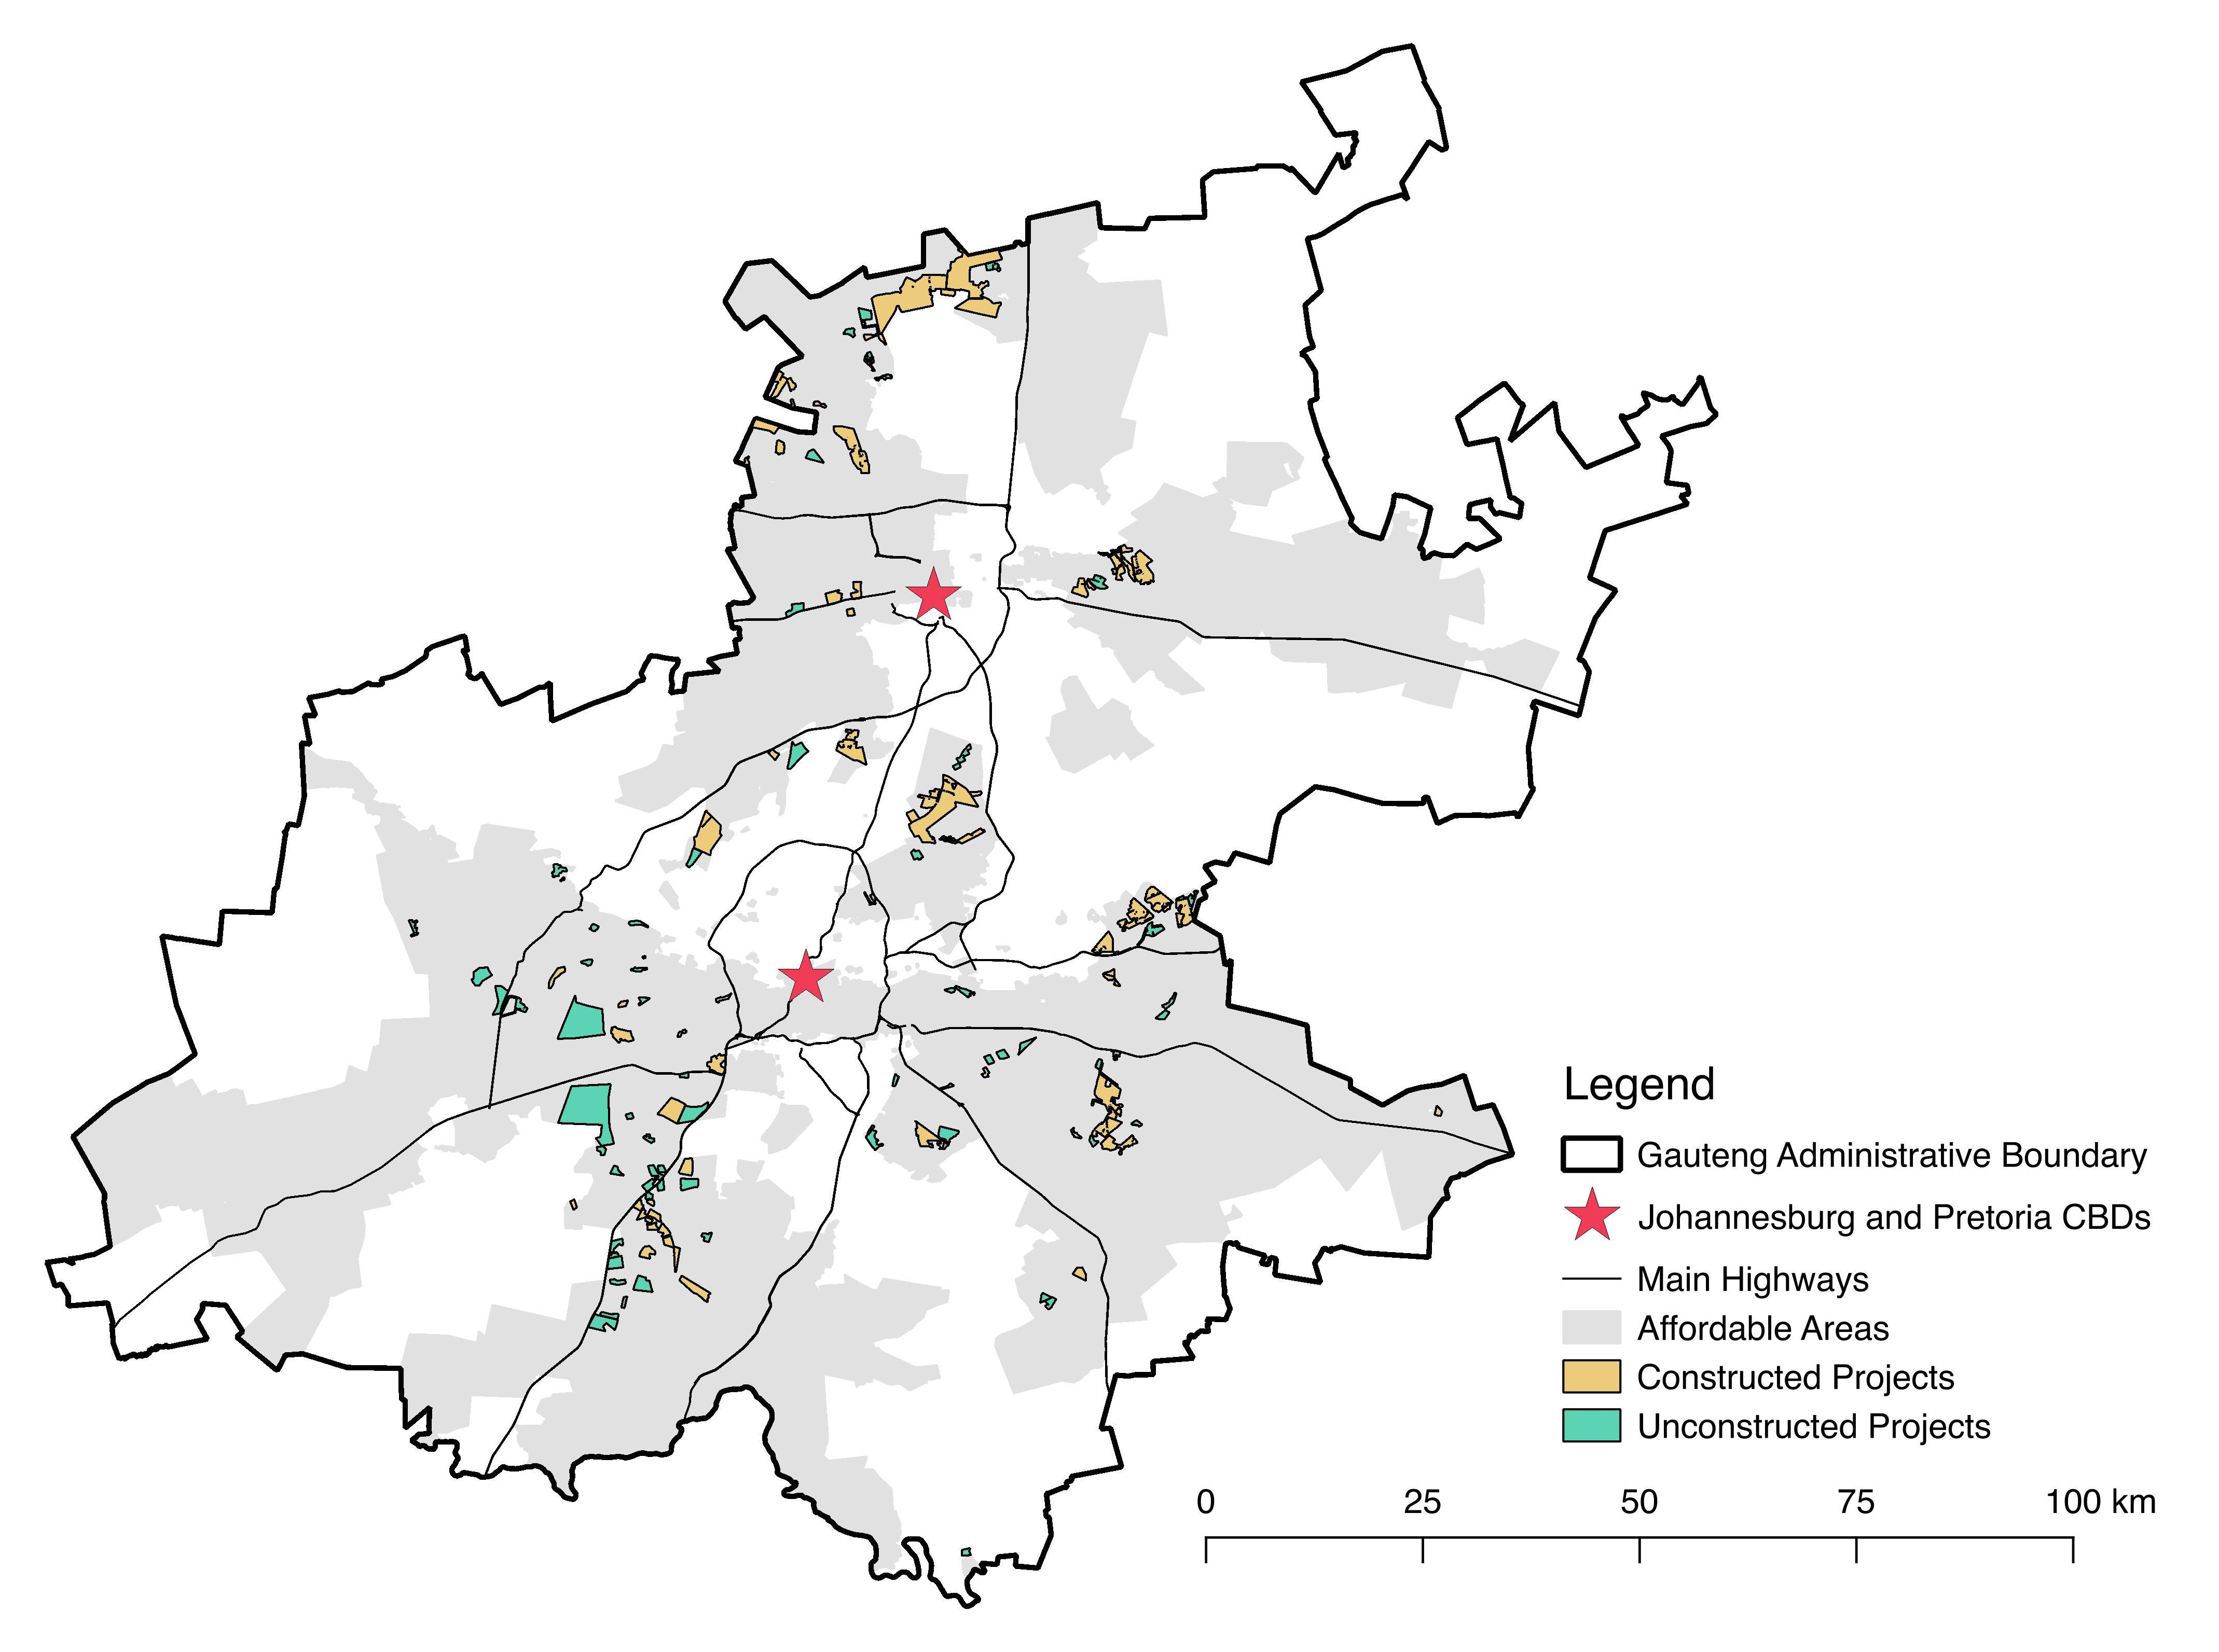
\includegraphics[scale=.098,trim={.9cm .4cm .9cm .4cm}]{figures/explanmap.jpg}}
\end{figure}



% Figure \ref{figure:map} shows the geographic setting of our analysis, displaying our final sample of constructed and unconstructed projects as polygons. Importantly, Figure \ref{figure:map} also shows that the affordable areas -- the coverage area for our deeds data -- contain every project boundary. While constructed and unconstructed projects are often adjacent to each other, possibly indicating cases where authorities were unable to complete final phases of planned projects, there are also many examples of isolated projects of both types.  Projects are generally located at relatively great distances from central business districts (CBDs), suggesting that vacant or inexpensive land plots are especially targeted by housing authorities.  Despite their distance from the CBDs, housing projects are often next to arterial highways, easing commuting costs for recipients.

% We note that our approach is not without limitations, and may introduce measurement error insofar as we are misattributing deeds to housing projects (false-positives), or assuming a project is unconstructed when it was actually constructed (false-negatives).  

% To provide some validation for our classification, we tabulate in Table~\ref{table:projectdescriptions} project descriptions from the 2008 administrative policy maps according to whether projects are classified as constructed or unconstructed by 2011.  As of 2008, we find that constructed projects are more likely to be classified as ``completed" or ``under implementation", while unconstructed projects are more likely to fall into ``proposed'' or ``planning'' categories.  Among constructed projects, we find 5 ``proposed'' and 8 ``planning'' indicators, which could imply either (1) these projects are false-positives or (2) while planned at some point prior to 2008, these projects were eventually completed by 2011.\footnote{We are unable to assess the frequency at which these descriptions are updated in the data.}  We also identify a single ``complete'' project as unconstructed, likely because its houses do not appear in our deeds records.  Figure \ref{fig:forchange} in section \ref{section:descriptives} further validates our sample, showing how formal housing increases disproportionately in projects classified as constructed. 




% \subsection{Nearby housing transactions}

To examine housing price spillovers nearby projects, we include properties that are located outside of the project areas and are not sold by government housing agencies or large developers identified as sellers with more than 30 transactions.  Excluding these sellers limits the external validity of our results only to small developers and individual homeowners.  We focus on properties located within 1.5 kilometers of constructed and unconstructed housing projects, forming a sample of over 67,000 transactions.  We exclude the top 1\% of prices as well as prices below 2,500 Rand, which are likely to be composed of mismeasured prices, or titles exchanged between family members. 


% \subsection{Census Data}

We measure impacts on dwelling and household characteristics with the full 1996, 2001, and 2011 Censuses of Population and Housing. We analyze average outcomes at the {\it small-area} level, the smallest available census geography. The province of Gauteng is divided between approximately 17,000 small-areas in 1996, 11,000 small-areas in 2001, and 17,000 small-areas in 2011, which are not constant over time periods.  On average, each small-area contains 170 households. 
% Though we observe responses from every surveyed household in both census waves, the data does not allow for linking households across time periods. 

% We analyze household-level responses describing the quality of their living quarters. 
% Our outcomes are mainly binary indicators and pertain to the household's access to services (flush toilets, water tap, electricity access), housing durability, and tenure arrangements. 
% We identify households 

\begin{figure*}[t!]
        \centering
        \caption[ Building-Based Land Use Data ]
        {\small Building-Based Land Use Data } 
        \vspace{2mm}
        \begin{subfigure}[b]{0.48\textwidth}
            \centering
            \frame{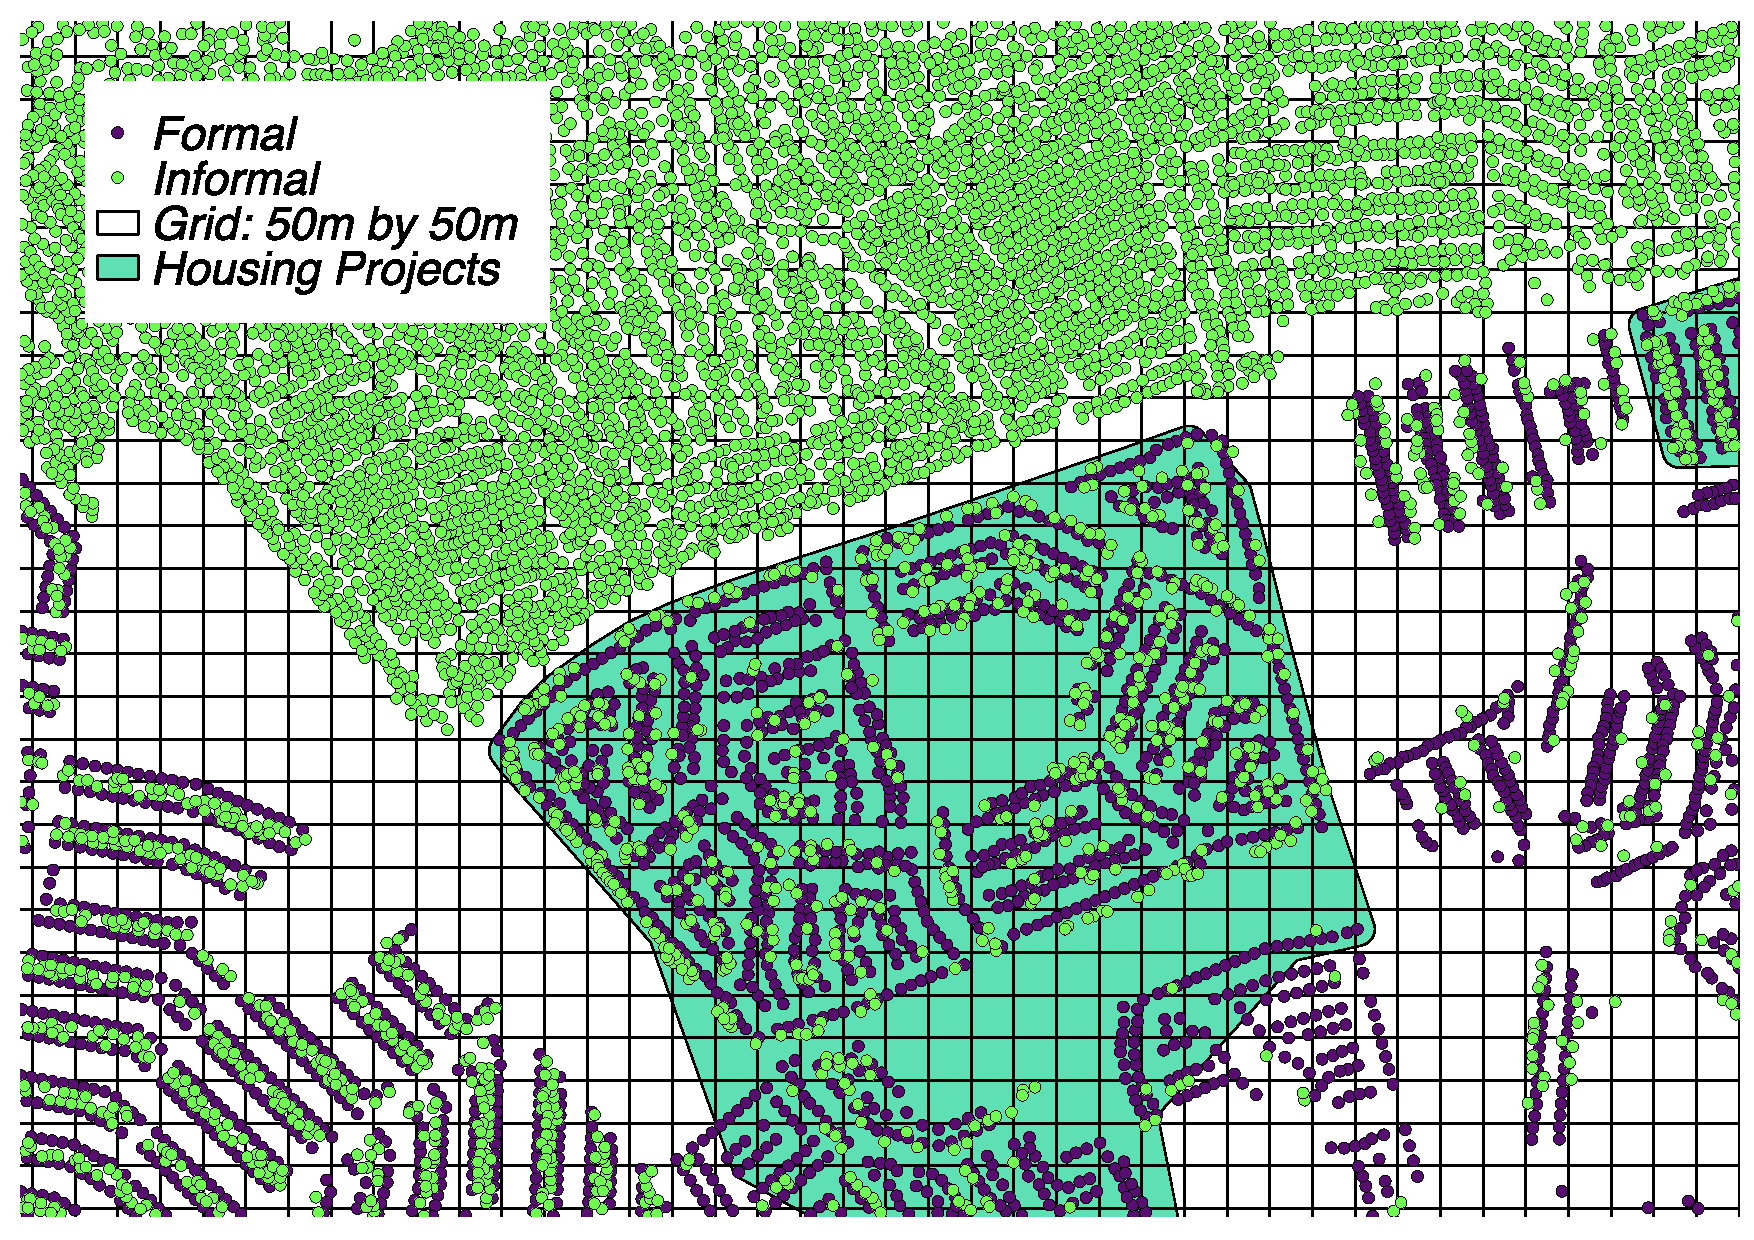
\includegraphics[width=\textwidth,trim={0cm 0cm 0cm 0cm}]{figures/bblu_map.jpg}}
            \caption[Network2]%
            {{\small raw data identifying (in)formal structures}}    
            %\label{fig:prefor}
        \end{subfigure}
        \hfill\quad
        \begin{subfigure}[b]{0.48\textwidth}  
            \centering 
            \frame{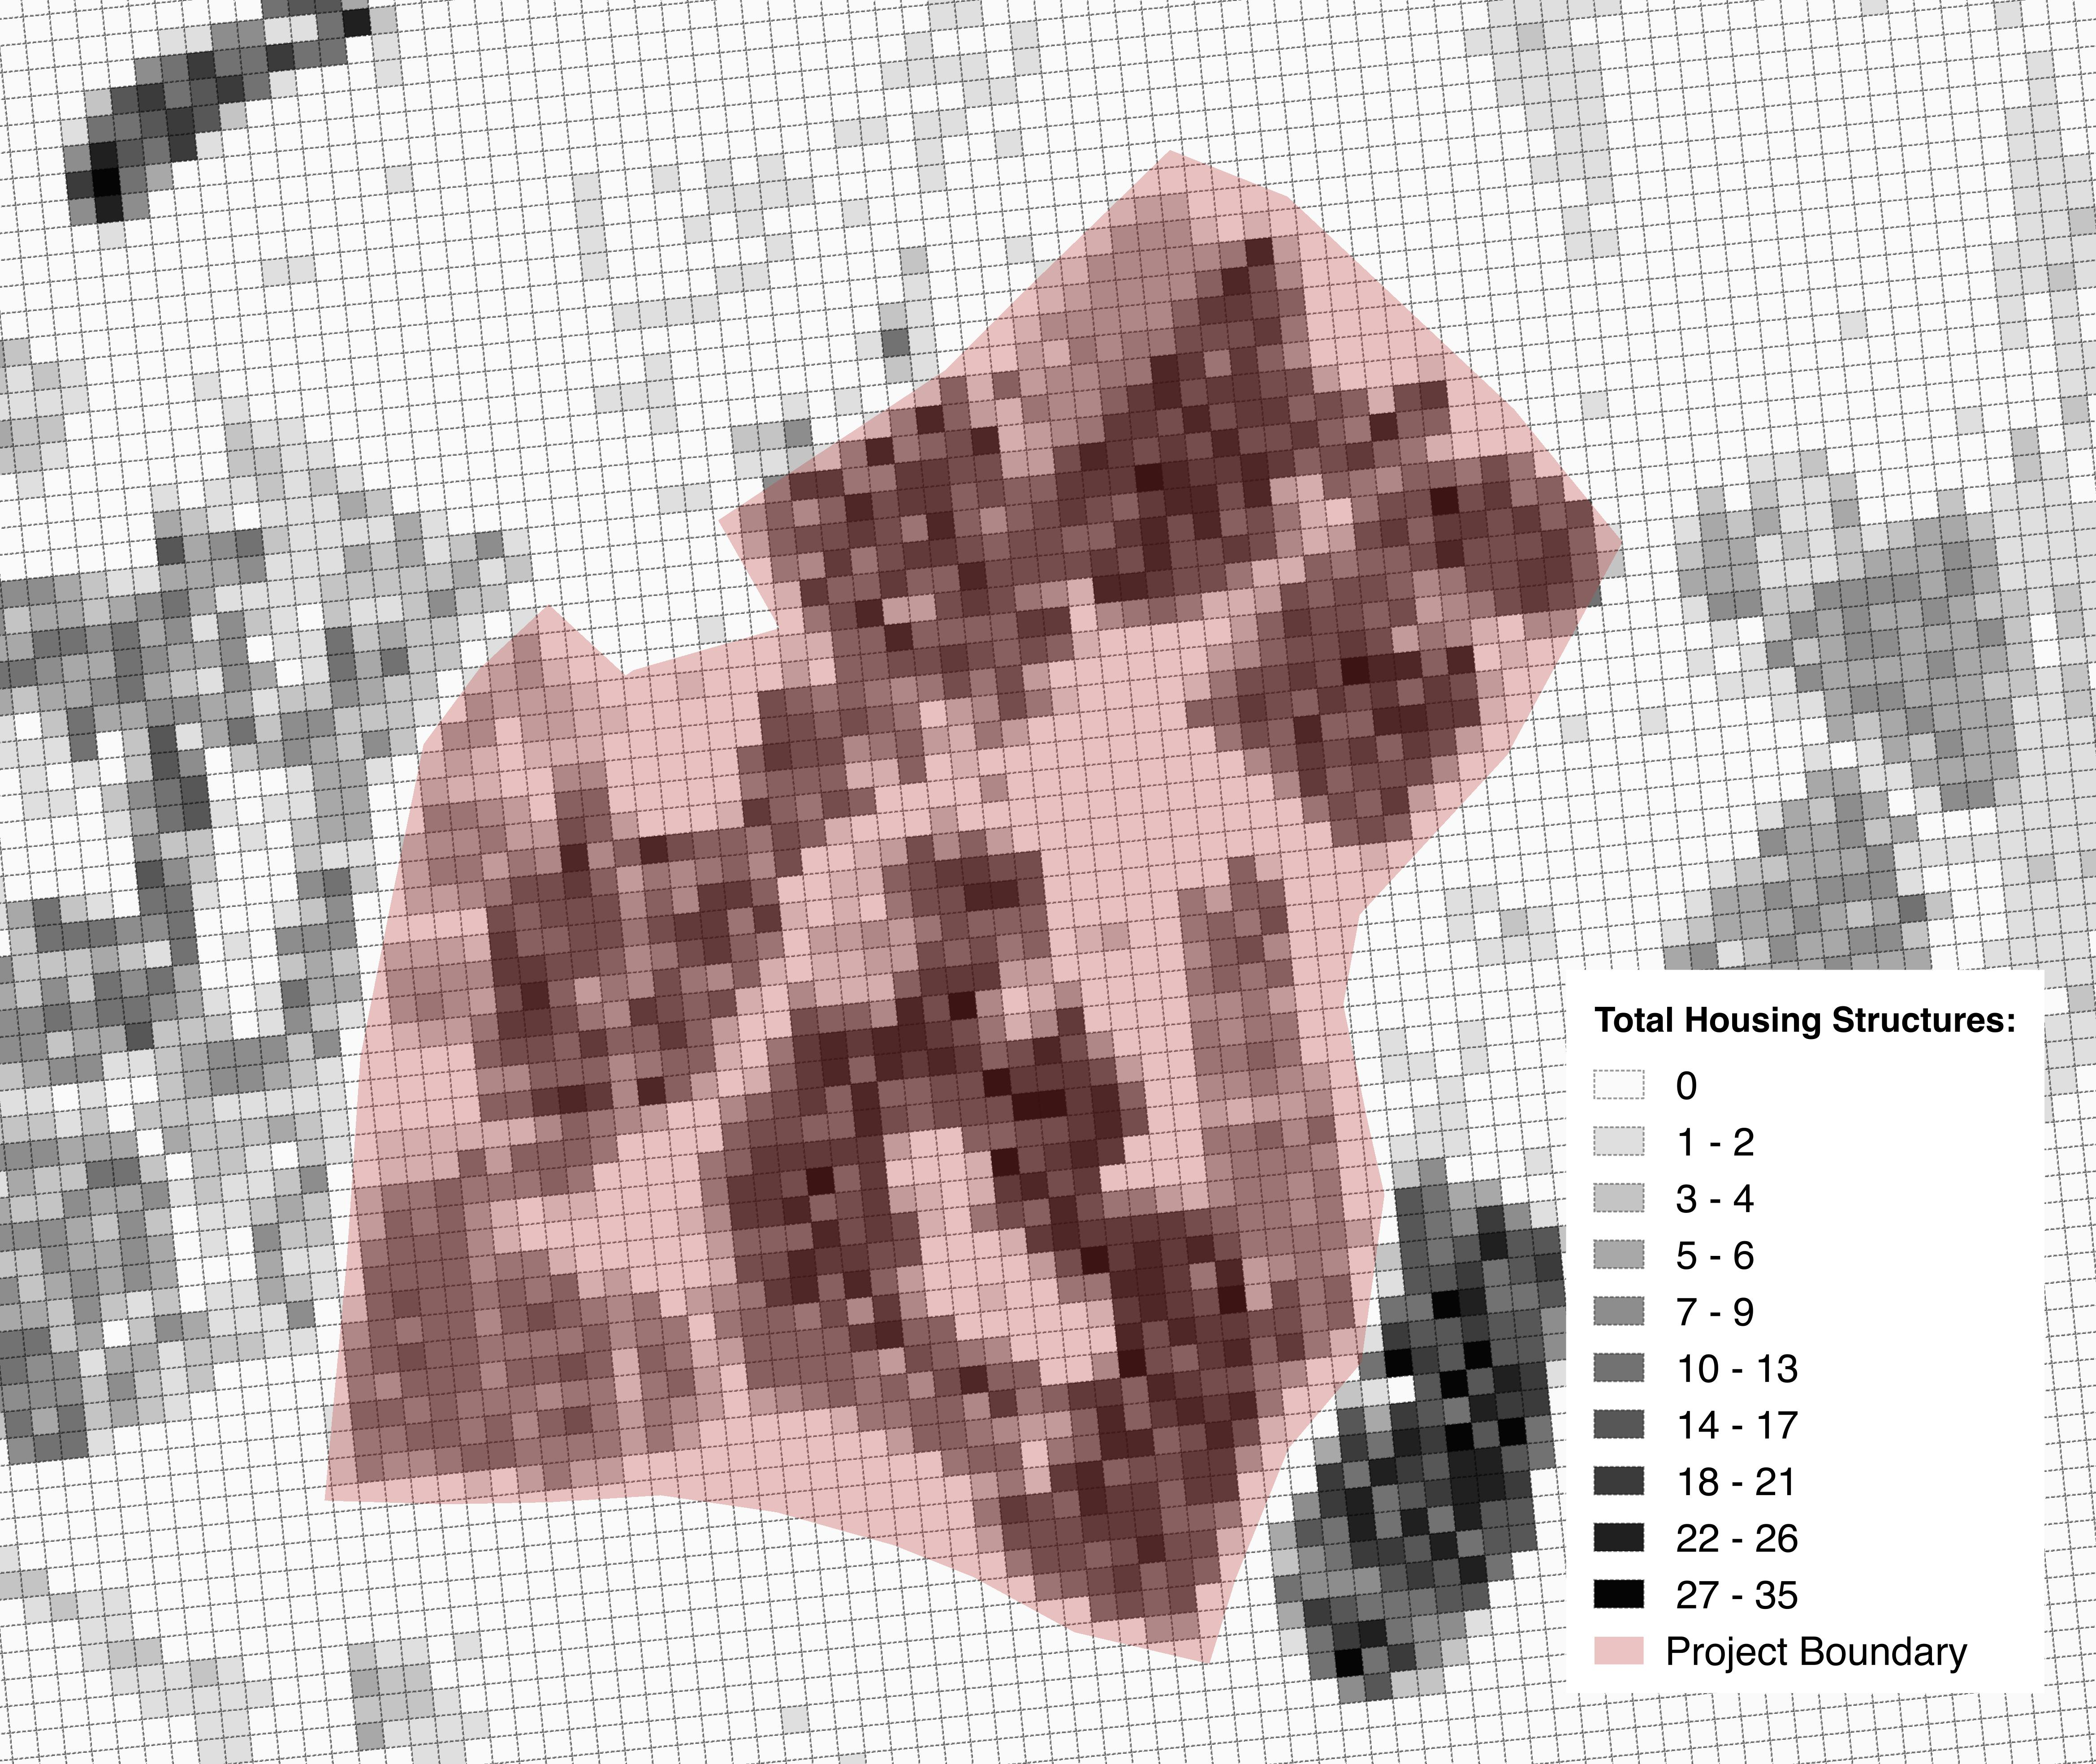
\includegraphics[width=\textwidth,trim={0cm 0cm 0cm 0cm}]{figures/bblu_grid.jpg}}
            \caption[]%
            {{\small 50$\times$50m grid cells data aggregation}}    
            %\label{fig:preinf}
        \end{subfigure}
        \label{fig:bblumaps}
    \end{figure*} 

% \subsection{Building Based Land Use}
% \label{section:data:bblu}

Our final data source consists of hand-coded building surveys derived from high-resolution aerial and satellite imagery. We obtain these data from GeoTerraImage (Pty) ltd., a local remote-sensing specialist.\footnote{\href{http://www.geoterraimage.com/}{\tt http://www.geoterraimage.com/}} The data differentiate structures across 30 categories, including formal and informal residential dwellings. Informal housing structures are easily identified from their temporary nature, often made of materials such as recycled wood and corrugated metal. In contrast, formal housing structures are permanent, generally made out of brick, and may have a pitched or a flat roof with tiles, zinc panels, or other materials. Importantly for our analysis, the data encodes backyard shacks as informal structures, but distinguishes between backyard and other types of informal buildings. We track changes in residential development by using two available survey waves in Gauteng: 2001 and 2012. As a validation exercise, we compute aggregated building counts at the census small-area level, and check the resulting figures against the number of households reporting to live in formal/informal housing in the census. The two data sources paint a consistent picture of housing in Gauteng, with high correlations ($\geq$ 0.85) between formal and informal building quantities in both available comparison years.\footnote{We correlate the 2001 and 2012 building surveys with the 2001 and 2011 censuses, respectively.} For estimation purposes, we transform this data into 25$\times$25m grid cell aggregates, creating five measures of housing density: (1) total residential structures split between (2) formal residential structures and (3) informal residential structures, which can be further decomposed into (4) backyard informal and (5) non-backyard informal structures.  In Figure \ref{fig:bblumaps}, we provide an example of the raw data and a depiction of our griding procedure, using the 2012 data wave.
% These grid cells will be the main units of observations for our housing density regressions, described in section \ref{section:bbluestimates}. 



\section{Descriptive Statistics}\label{section:descriptives}
% As mentioned in section \ref{section:data}, 
% Validate measures :
% \begin{itemize}
% 	\item delivered houses are way higher in constructed, but there's a little room for slippage
% \end{itemize}
% Balance/identification discussion : 
% \begin{itemize}
% 	\item everything else is really balanced, which is good for identification
% \end{itemize}

% Spatial targeting

% Unconstructed and constructed Differences

% Which types of neighborhoods receive unconstructed and constructed projects and where are projects located within neighborhoods

We provide descriptive evidence to first validate our measures of constructed and unconstructed projects.  We then examine differences between neighborhoods with constructed projects and neighborhoods with unconstructed projects.  We also examine where projects are located within neighborhoods.  Finally, we document how project areas and nearby areas evolve differentially over time.  

Table~\ref{table:projectdescriptives} compares average attributes for constructed and unconstructed projects.  The first row counts the number of project houses recorded in the deeds data within constructed and unconstructed projects, providing an independent measure of which projects were constructed.  Projects categorized as constructed receive a large influx of 374 deeds project houses between 2001 and 2011, indicating that many of these projects were successfully completed in this interval.  By contrast, projects categorized as unconstructed receive just 11 deeds project houses on average, which suggests that completed projects are unlikely to be misclassified as unconstructed projects.   

Housing prices within 1km of projects are lower than the average price of 252,000 Rand for areas over 1 km from projects, indicating that projects are located in neighborhoods with less expensive land.  With average land areas exceeding one km2, housing projects represent a significant change to local neighborhoods.  Size, timing, location, and nearby house prices are broadly similar between unconstructed and constructed projects.  

% All other attributes of housing 
%  the location, size, and surrounding housing stock of the 317constructed and unconstructed projects.  shows that constructed projects deliver an average of 374 houses as measured by the deeds data.  By contrast, projects flagged as unconstructed only produce 11 houses on average, suggesting that 
% validated also by the descriptive changes in housing projects... 
% Constructed projects are also substantially larger in area than unconstructed projects. these discrepancies may be due to many unconstructed projects representing smaller planned extensions to previously implemented projects. 
% It may also reflect the fact that larger land plots are first targeted by housing authorities to maximize delivery. 
% Though unconstructed projects are located in slightly more remote locations, both types of projects impose long commutes on residents, as measured by the average distance to central business districts. 
% These distances are consistent with housing authorities targeting inexpensive, vacant land for these projects. Finally, prices for non-subsidized housing in the vicinity of project boundaries are slightly lower for unconstructed projects, perhaps driven in part by their more distant locations.
% Table~\ref{table:projectdescriptives} further divides projects into city and suburb according to whether their centroids are above or below median distance from a CBD respectively.  City projects are smaller, but receive more houses than suburb projects.  We also find higher housing prices in formal markets surrounding project areas consistent with these areas providing better access to employment opportunities.  Similar patterns emerge between constructed and unconstructed projects when we disaggregate by distance to CBD.

\vspace{0mm}
\begin{table}[h!]
\centering
\caption{Housing Project Areas Description}\label{table:projectdescriptives}
\vspace{0mm}
\begin{tabular}{l*{1}{cc}}
\toprule
  &Constructed & Unconstructed \\
\midrule
 Number of Projects  & 164  & 137  \\ 
 Area (km2)  & 1.21  & 1.19  \\ 
 Median Construction Year  & 2006  & 2006  \\ 
 Delivered Houses  & 302  & 0  \\ 
 House Price within 1km (Rands$^\dagger$)  & 189,304  & 218,635  \\ 
 Distance to CBD$^\ddagger$ (km)  & 32.4  & 28.0  \\ 

\bottomrule
%\multicolumn{3}{l}{\scriptsize Const. refers to constructed projects and unconst. refers to unconstructed projects.}\\[-.5em]
%\multicolumn{3}{l}{\scriptsize $^*$Calculated from {\it expected} completion dates using Gauteng National Treasury budget reports.}\\[-.5em]
\multicolumn{3}{l}{\scriptsize $^\dagger$ The USD averaged around 7.70 Rands during the 2001-2011 period.}\\[-.5em]
\multicolumn{3}{l}{\scriptsize $^\ddagger$Measured as the average minimum distance with respect to Johannesburg and Pretoria CBDs. } \\[-.5em]
\end{tabular}
\end{table} 


% Next, we turn to household census data to assess how both types of projects differ in terms of dwelling characteristics prior to project construction. 

To further assess where projects are located, Table~\ref{table:projectdescriptivescensus} uses pooled 1996 and 2001 census data to examine preexisting housing quality for project footprints before construction.  Since census small-areas are often larger than housing projects, Table~\ref{table:projectdescriptivescensus} considers census small-areas as pertaining to a housing project when over 50\% of the land area of the small-area overlaps with a project footprint.\footnote{Our census geography selection method is depicted in more detail in appendix \ref{appendix:bufferdesign}.}  Table~\ref{table:projectdescriptivescensus} compares means for household indicators aggregated at the small-area level based on whether the census boundaries overlap with constructed (first column) or planned but unconstructed projects (second column).  As a reference, the third column provides averages for all census small-areas in the Gauteng province.

\begin{table}[h!]
	\centering
	\caption{Mean Housing Characteristics from the 1996 and 2001 Censuses}\label{table:projectdescriptivescensus}
\vspace{-2mm}
\begin{tabular}{l*{1}{ccc}}
\toprule
& Constructed & Unconstructed & All small-areas \\
\midrule
Flush Toilet&0.86&0.68&0.82 \\
Piped Water in Home&0.48&0.20&0.42 \\
Electricity for Cooking&0.79&0.42&0.71 \\
Electricity for Heating&0.76&0.37&0.68 \\
Electricity for Lighting&0.85&0.63&0.80 \\
Number of Rooms&3.69&2.81&3.51 \\
Household Size&3.48&3.44&3.47 \\
\% Area Overlap with Projects&0.97&0.89&0.65 \\
N&          5,391&          1,400&          6,834 \\
 
\bottomrule
\multicolumn{4}{l}{\scriptsize ``Constructed'' and ``Unconstructed'' include census small-areas with over 50\% } \\ [-.5em]
\multicolumn{4}{l}{\scriptsize  area overlap with constructed and unconstructed projects respectively. } \\ [-.5em]
\multicolumn{4}{l}{\scriptsize ``All''  includes all small-areas.  Means are weighted by land area.}
\end{tabular}
\end{table}


Table \ref{table:projectdescriptivescensus} finds that before project construction, preexisting houses in project footprints are smaller and less formal with worse access to services compared to other houses in the province.  This finding is consistent with efforts by the Gauteng government to locate housing projects in inexpensive, poorer neighborhoods to both upgrade these neighborhoods as well as save costs.  Comparing preexisting houses in constructed and unconstructed projects, we do not observe systematic differences in housing attributes.  While constructed project footprints are more likely to have flush toilets, electricity, and large household sizes, households in unconstructed project footprints report having better access to formal houses and piped water in their homes.  With a small number of small-areas, average characteristics are not statistically different between constructed and unconstructed project footprints except for the formal housing measure.\footnote{Statistical significance is calculated at 5\% confidence level weighted by land area.}

% Despite some similarities between averages in constructed and unconstructed areas, a simple t-test rejects the null hypothesis that means are equal for every tabulated variable.  

%Appendix Table~\ref{table:projectdescriptivescensushet} compares characteristics for constructed and unconstructed areas separately for projects in city centers and in suburbs, broadly similar patterns between constructed and unconstructed areas at baseline.
% Given the low-quality of land plots that were targeted by this policy, we expect project areas to lag behind other areas, and reflect more precarious housing conditions.  
% We find that access to sanitation, water and electricity are between 30 and 70\% lower in both types of project areas relative to the province as a whole. 
%\footnote{Row 3 of table \ref{table:censusestimates} tests identical null hypotheses in a regression framework that allows for arbitrary correlations between observations within the same project, and cannot reject equality for all outcomes except household size.}



\begin{figure*}[h!]
        \centering
        \caption[ 2001 Housing Densities in Constructed and Unconstructed Projects]
        {\small 2001 Housing Densities in Constructed and Unconstructed Projects} 
        %\vspace{2mm}
        \begin{subfigure}[b]{0.495\textwidth}
            \centering
            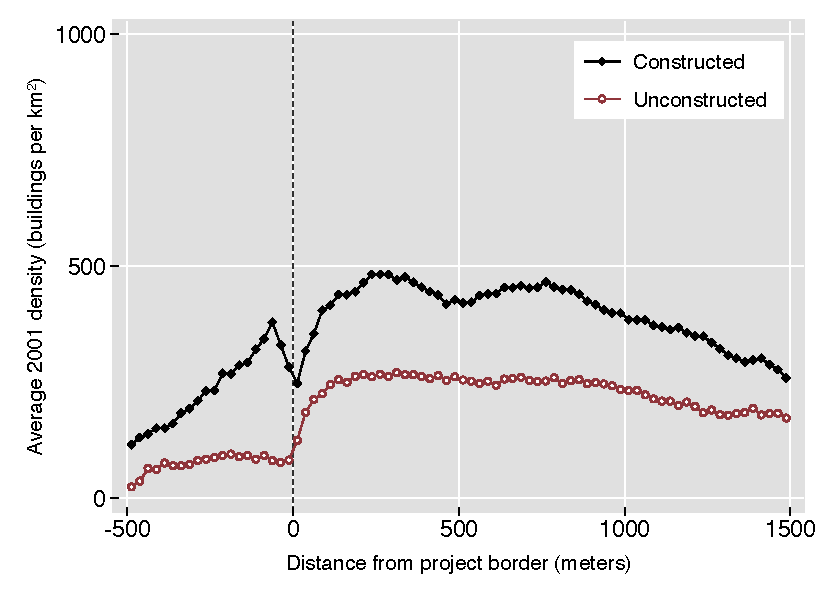
\includegraphics[width=\textwidth,trim={0.3cm .3cm 0.1cm 0cm}, clip=true]{figures/bblu_for_pre_means_4_spk.pdf}
            \caption[Network2]%
            {{\small Formal density}}    
            \label{fig:prefor_raw}
        \end{subfigure}
        \hfill
        \begin{subfigure}[b]{0.495\textwidth}  
            \centering 
            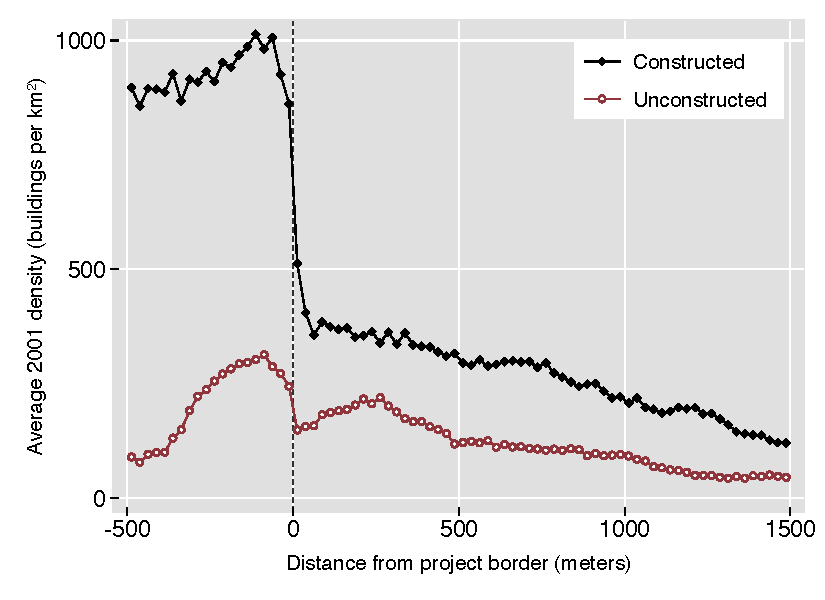
\includegraphics[width=\textwidth,trim={0.3cm .3cm 0.1cm 0cm}, clip=true]{figures/bblu_inf_pre_means_4_spk.pdf}
            \caption[]%
            {{\small Informal density}}    
            \label{fig:preinf_raw}
        \end{subfigure}
        \begin{subfigure}[b]{0.495\textwidth}
            \centering
            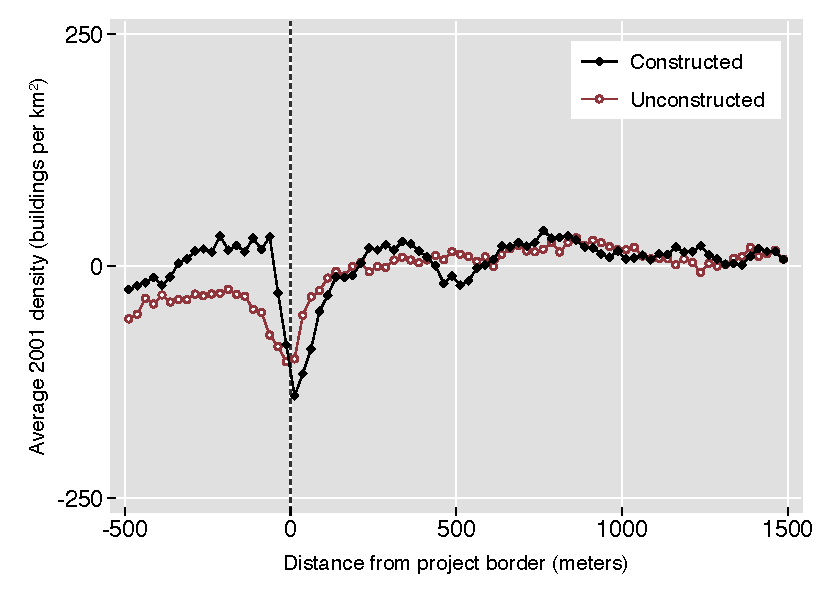
\includegraphics[width=\textwidth,trim={0.3cm .3cm 0.1cm 0cm}, clip=true]{figures/bblu_for_fe_pre_means_4_spk.pdf}
            \caption[Network2]%
            {{\small Formal density within neighborhood}}    
            \label{fig:prefor_fe}
        \end{subfigure}
        \hfill
        \begin{subfigure}[b]{0.495\textwidth}  
            \centering 
            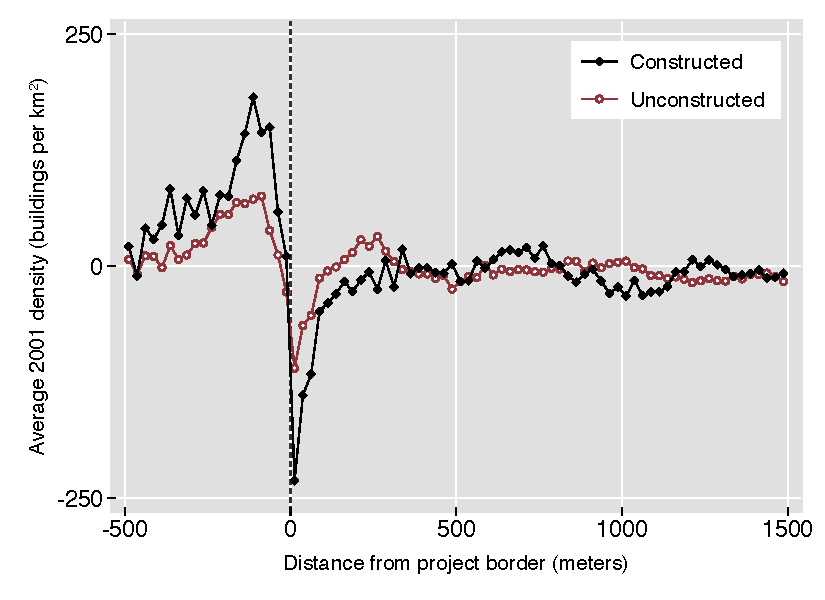
\includegraphics[width=\textwidth,trim={0.3cm .3cm 0.1cm 0cm}, clip=true]{figures/bblu_inf_fe_pre_means_4_spk.pdf}
            \caption[]%
            {{\small Informal density within neighborhood}}    
            \label{fig:preinf_fe}
        \end{subfigure}
        \label{fig:rawbblumeans_het}
        %\vspace{-6mm}
   {\scriptsize Negative distances indicate areas within project boundaries while positive distances measure areas away increasingly outside of project boundaries.  Within neighborhood densities are calculated by subtracting mean densities  \\[-.5em] at the 2001 census subplace level from each 25$\times$25m grid cell.}
    \end{figure*} 

% Using the building-based land-use measures described in section \ref{section:data:bblu}, 
% we then examine housing densities across constructed and unconstructed project areas.  
% To inspect how densities change with proximity to housing projects,
% Probably worth commenting on this gap in the pre-period inside the boundaries.

The building-based land-use data complement the census data by providing a spatially precise measure of preexisting development in areas prior to project construction.  We calculate euclidean distances from the centroid of 25$\times$25m grid-cells to the nearest project boundary, assigning negative distances to grid-cells inside project footprints.  We then compute the average density at 25m intervals, reported in houses per square kilometer.\footnote{Greater negative distances exclude smaller projects in computing average densities, which may account for some of the variation in building density within projects, particularly for informal housing.  Appendix~\ref{appendix:projectcounts} illustrates this compositional change in more detail.} 

Figures \ref{fig:prefor_raw} and \ref{fig:preinf_raw} respectively plot average preexisting densities of formal and informal houses in 2001. We find low densities of formal housing and very high densities of informal housing within both unconstructed and constructed project footprints (at negative distances).  Crossing just outside of project footprints (to positive distances), formal housing densities quickly increase while informal housing densities sharply jump downwards.  These trends are consistent with housing projects being precisely targeted within poorer neighborhoods with few existing formal dwellings.  Formal and informal housing densities gradually decay moving further from project footprints.  On average, constructed projects are located in neighborhoods with greater housing densities than unconstructed projects although housing densities following similar trends with respect to distance from project boundaries.  Informal densities within project footprints are significantly higher for constructed projects compared to unconstructed projects, which is consistent with housing authorities prioritizing project completion in neighborhoods with large slums (\cite{hofmeyr2008risk}).  

Given that housing projects appear to be located in inexpensive neighborhoods with high preexisting densities of informal housing, we next examine whether housing projects are further targeted to particular locations within neighborhoods.  Figures \ref{fig:prefor_fe} and \ref{fig:preinf_fe} are calculated by first subtracting the average housing density in each neighborhood from the density in each grid cell, then calculating averages over distance to project footprints.  Neighborhoods are defined according to 1,001 census 2001 subplaces, which identify suburbs, wards, villages, or informal settlements (\cite{censusmeta}).  Figures \ref{fig:prefor_fe} and \ref{fig:preinf_fe} can be interpreted as the difference in housing density from the neighborhood average associated with each distance from a project boundary.  

Accounting for neighborhood differences removes much of the variation in preexisting housing densities across distances to housing projects, especially outside of project footprints.  Yet, low levels of formal housing and high levels of informal housing persist just within project footprints, consistent with housing authorities targeting inexpensive, poorer plots of land for housing projects.  Similar patterns within neighborhoods for constructed and unconstructed areas suggest that both project types are located using similar criteria.  Accounting for neighborhood densities collapses average differences in densities between constructed and unconstructed projects although constructed projects have higher building densities within project footprints.  

% Appendix Table~\ref{fig:rawbblumeans_het} graphs pre-period density of formal and informal housing separately for projects in city centers and projects in suburbs.  Unconstructed project areas near city centers have slightly higher densities of informal housing and lower densities of formal housing.  In suburbs, the opposite pattern holds with constructed project areas having somewhat higher densities of formal housing and lower densities of informal housing.  Outside of project boundaries, constructed and unconstructed projects have similar informal and formal housing levels in both city and suburb areas.

\begin{figure*}[t!]
        \centering
        \caption[ Changes in Housing Densities in Constructed and Unconstructed Projects Areas]
        {\small Changes in Housing Densities in Constructed and Unconstructed projects } 
        %\vspace{2mm}
        \begin{subfigure}[b]{0.495\textwidth}   
            \centering 
            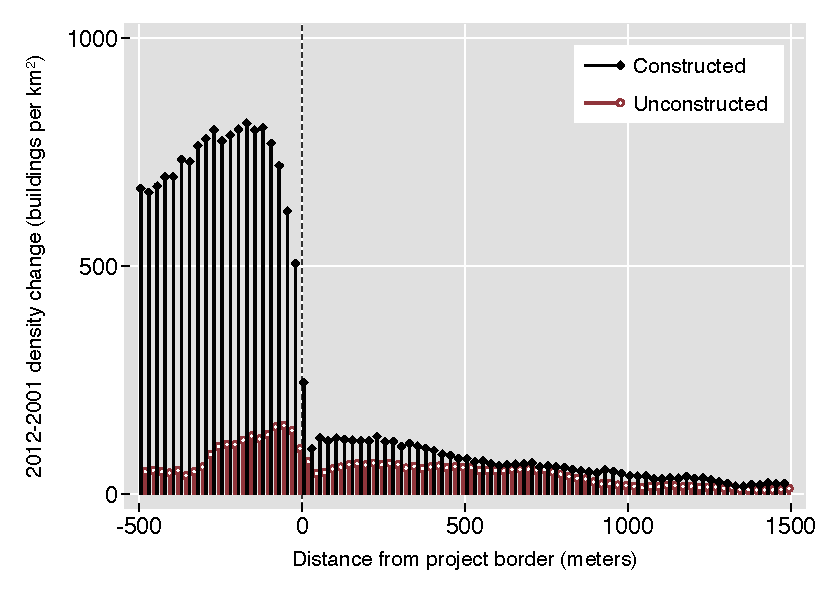
\includegraphics[width=\textwidth,trim={0.3cm .3cm 0.1cm 0cm}, clip=true]{figures/bblu_for_rawchanges_4_spk}
            \caption[]%
            {{\small formal housing density change}}    
            \label{fig:forchange}
        \end{subfigure}
        \hfill
        \begin{subfigure}[b]{0.495\textwidth}   
            \centering 
            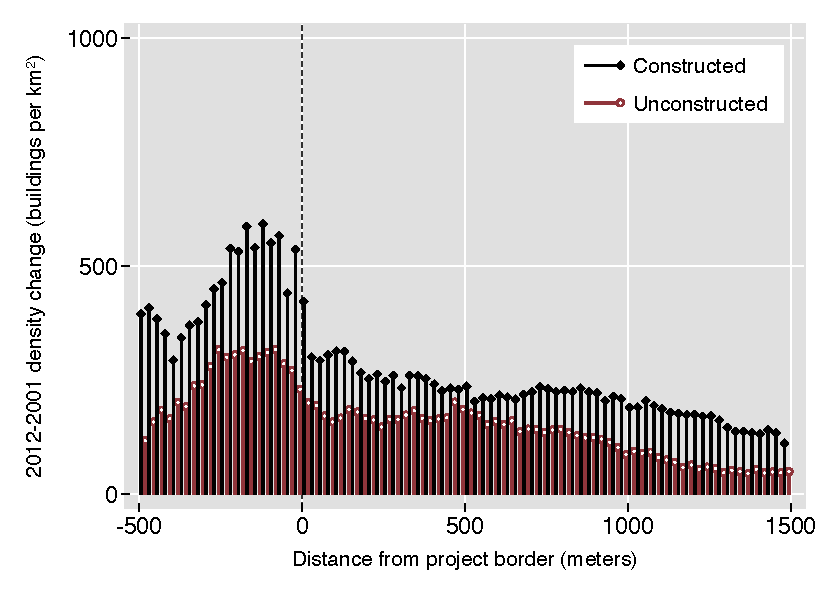
\includegraphics[width=\textwidth,trim={0.3cm .3cm 0.1cm 0cm}, clip=true]{figures/bblu_inf_rawchanges_4_spk}
            \caption[]%
            {{\small informal housing density change}}    
            \label{fig:infchange}
        \end{subfigure}
        \label{fig:rawbblumeanschange}
        \vspace{-6mm}
    \end{figure*} 

To examine how project areas evolve over time, Figures \ref{fig:forchange} and \ref{fig:infchange} are constructed by computing the change in building density for each grid cell from 2001 to 2012 and then averaging these changes according to distances to project boundaries.  Both formal and informal housing densities increase over this time period, reflecting rapid urbanization throughout the Guateng province.  

Growth in formal housing is concentrated within constructed project footprints, dropping abruptly at project boundaries (at zero distance).   This trend is consistent with housing projects producing large amounts of new, formal housing  (\cite{dhsreports}).  Sharp changes in formal housing growth at project boundaries are also consistent with having a precise measure of housing project boundaries.\footnote{In contrast, an imprecise measure that misclassifies some non-project areas as project areas (and vice versa) would predict a smooth average trend in formal housing changes across footprint boundary.}  Compared to constructed projects, unconstructed projects experience much less growth in formal housing within their footprints.  This finding confirms their status as planned, but unconstructed.  Moving from within footprints to outside of footprints, unconstructed projects observe declining formal housing growth.  Since projects are often located on undeveloped land, private housing development may crowd into these areas in the absence of housing project construction.  Moving further from project boundaries, formal housing growth decays similarly between constructed and unconstructed areas.

 % Alternatively, this growth in formal housing may represent measurement error where some projects that are classified as unconstructed were actually finished between 2001 and 2012.

Growth in informal housing density is higher within than outside of project footprints as shown by Figure~\ref{fig:infchange}.  This result is unsurprising for unconstructed projects:  informal settlements grow in underdeveloped, inexpensive land in the absence of project construction.  Yet, for constructed projects, this result suggests that even after authorities have cleared the existing informal housing stock to make way for housing projects, total informal housing growth still exceeds growth in unconstructed project areas.  Moving further from footprints, growth in informal housing decays with distance at a faster rate for unconstructed projects than for constructed projects.  


% Informal housing now!!!   We might think that informal housing should decline as areas are bulldozed!  BUT 
% DO DENSITIES TO THE CLOSEST PROJECT! ( TO SEE THE DECAY EVIDENT IN THE REGRESSIONS!!! )

% The effect of the policy is clearly evidenced in figure \ref{fig:forchange}, where tall black bars at negative distances show increases in the density of formal housing of around 1,000 structures per $\text{km}^{2}$ within constructed project areas.  Compared to a baseline mean density of about 400 structures per $\text{km}^{2}$ in Figure \ref{fig:prefor}, this shift represents a nearly 250\% increase. In contrast, unconstructed areas (red bars) experience increases in formal housing density at much smaller rates.
% %Importantly, density changes at negative distances for unconstructed areas resemble changes outside of project areas in magnitude, consistent with a broader secular expansion in housing.
% At positive distances, both series are almost overlapping.  This result previews our empirical analysis by showing little evidence of spillover effects on neighboring formal housing markets.

% In figure \ref{fig:infchange}, we observe large increases in informal density within project boundaries for both constructed and unconstructed project areas.  At some distances, unconstructed projects appear to overtake constructed areas in informal housing growth.  Outside of project boundaries, constructed areas experience larger increases in informal density than unconstructed areas. With the exception of 0-200m, these increases do not appear to be systematically different between the treated and control ares. 
% %This absence of differential trends with distance previews a similar absence of spillover effects for informal housing densities explored further in the empirical analysis.
% Relative to baseline levels in Figure \ref{fig:preinf}, informal housing increases are large, increasing by at least 50\% across all distances and nearly doubling in some cases.



\begin{figure*}[t!]
        \centering
        \caption[ House prices outside constructed and unconstructed projects ]
        {\small House prices outside constructed and unconstructed projects } 
        %\vspace{2mm}
        \begin{subfigure}[b]{0.495\textwidth}
            \centering
            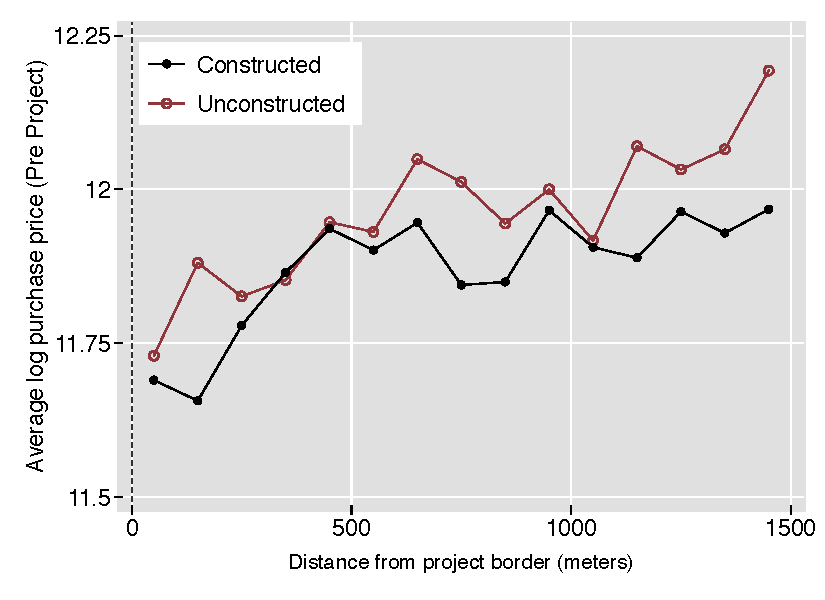
\includegraphics[width=\textwidth,trim={0.9cm .3cm 0.1cm 0cm}, clip=true]{figures/price_pre_means_4}
            \caption[Network2]%
            {{\small pre-period log-prices }}    
            \label{fig:preprice}
        \end{subfigure}
        \hfill
        \begin{subfigure}[b]{0.495\textwidth}   
            \centering 
            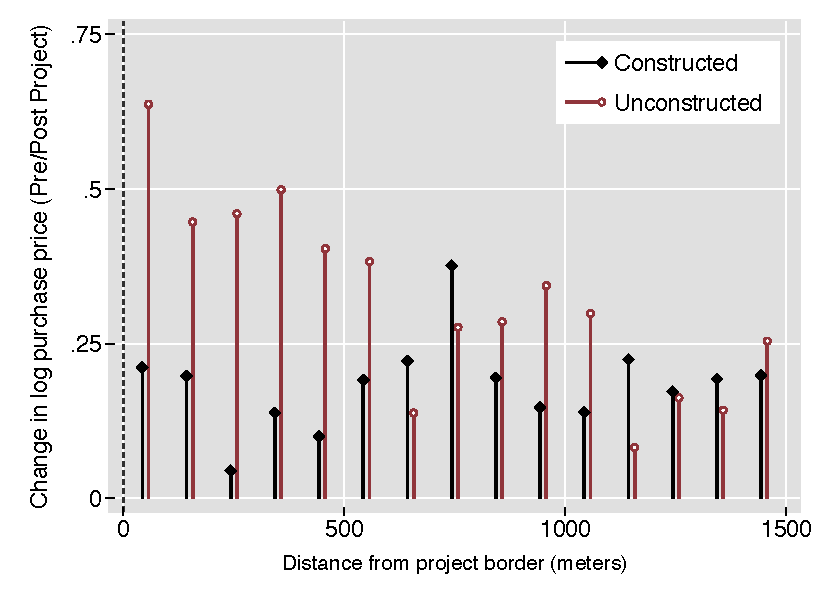
\includegraphics[width=\textwidth,trim={0.9cm .3cm 0.1cm 0cm}, clip=true]{figures/price_rawchanges_4}
            \caption[]%
            {{\small change in log-prices}}    
            \label{fig:changeprice}
        \end{subfigure}
        \label{fig:rawpricemeans}
        \vspace{-6mm}
\end{figure*} 


Figure~\ref{fig:rawpricemeans} performs an analogous exercise with property transaction data from the deeds records.  These records are likely to be composed of formal houses because informal housing transactions are rarely recorded.  Since there are very few non-subsidized housing transactions within project footprints, we focus only on transactions at positive distances.  Using the date of each transaction, we group prices before and after the expected completion dates for both constructed and unconstructed projects. 
% To make comparisons within a normalized timeline, we first residualize log purchase prices from year$\times$month and project fixed effects.

Figure~\ref{fig:preprice} plots average log purchase prices before the expected completion date for both constructed and unconstructed areas with respect to distance to project footprints.  Moving from 0 to 1,500 meters from project footprints, prices increase by about 0.3 log-points or roughly 30\% for both constructed and unconstructed projects.  Low prices near project boundaries are consistent with reports of public housing officials targeting low-cost land for housing development.  Figure~\ref{fig:changeprice} graphs average changes in log-purchase prices before and after the expected completion of projects with respect to distance to project footprints.  While prices increase overall, prices near unconstructed footprints increase more than prices for constructed footprints, especially within 500 meters from footprints.  


\begin{figure*}[t!]
        \centering
        \caption[ Average house prices before and after expected construction ]
        {\small Average house prices before and after expected construction } 
        %\vspace{2mm}
        \begin{subfigure}[b]{0.495\textwidth}
            \centering
            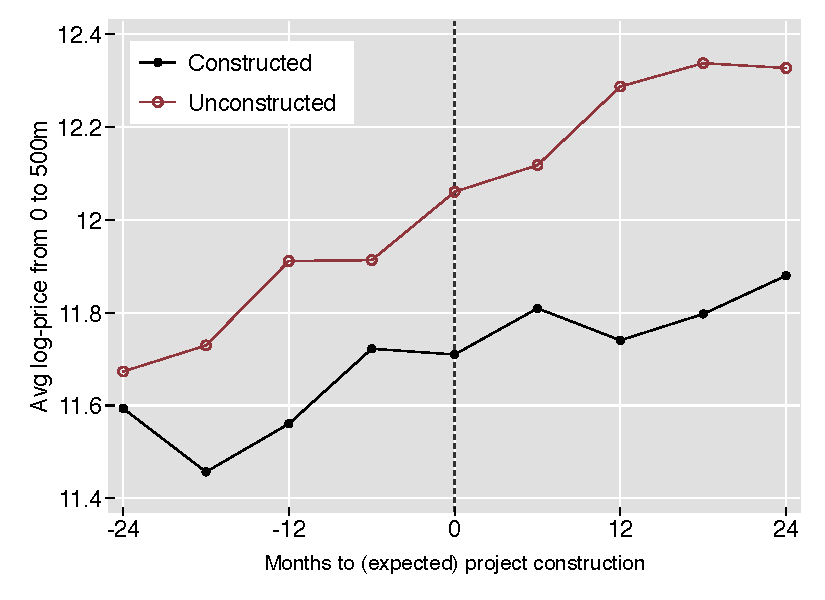
\includegraphics[width=\textwidth,trim={0.9cm .3cm 0.1cm 0cm}, clip=true]{figures/price_pretrends_close__4}
            \caption[Network2]%
            {{\small log-prices 0 to 500m from projects}}    
            \label{fig:pretrend_close}
        \end{subfigure}
        \hfill
        \begin{subfigure}[b]{0.495\textwidth}   
            \centering 
            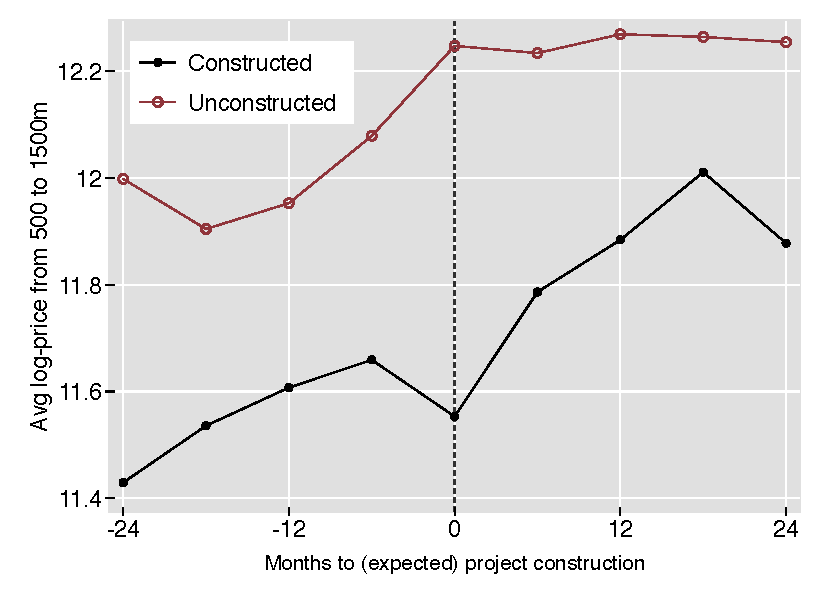
\includegraphics[width=\textwidth,trim={0.9cm .3cm 0.1cm 0cm}, clip=true]{figures/price_pretrends_far__4}
            \caption[]%
            {{\small log-prices 500 to 1,500m from projects}}    
            \label{fig:pretrend_far}
        \end{subfigure}
        \label{fig:pretrend}
        \vspace{-6mm}
\end{figure*} 


Deeds data contain the exact date of each housing transaction, which allows us to examine how local housing prices vary with respect to the completion date for constructed projects and the expected completion date for unconstructed projects.  Figure~\ref{fig:pretrend_close} plots average log-prices for housing transactions between 0 and 500 meters outside project footprints from two years before and after completion date.  Within 500 meters, prices for constructed and unconstructed projects follow roughly parallel trends prior to project completion.  Prices diverge after completion with prices near unconstructed projects rising more quickly than prices near constructed projects.  Figure~\ref{fig:pretrend_far} includes the analogous plot for housing transactions located 500 to 1,500 meters from project footprints.  Again, both constructed and unconstructed prices follow parallel trends prior to completion, following similar slopes to their corresponding plots in Figure~\ref{fig:pretrend_close}.  After completion, price growth slows for areas near unconstructed projects, shrinking the gap between prices near constructed and unconstructed projects.  Taken together, Figure~\ref{fig:pretrend_close} and Figure~\ref{fig:pretrend_far} do not provide strong evidence for pretrends in prices in anticipation of project construction.  

% Prices within 500 meters of unconstructed projects maintain a steady, increasing trend two years before and after expected project completion.  

% Prices for constructed and unconstructed projects also follow similar levels and trends before construction.
% We document an increase in prices of about 0.2 log-points or roughly 20\% for unconstructed project areas. The picture is less clear for constructed projects, which show an increasing price gradient within the first 500m, but exhibit noisy patterns further away.  Overall, both series show large variations in house prices, which make it difficult to identify  distinct patterns.
% The steady increase observed for unconstructed project areas is consistent with findings in table \ref{table:projectdescriptivescensus} that project areas (both constructed and unconstructed) fare worse in terms of indicators of housing quality.
% we observe some evidence that unconstructed areas experience a boom in nearby housing prices that was not mirrored by constructed areas.  Yet, this gap quickly closes, further suggesting that housing projects play a minimal role in driving nearby housing markets.




\section{Empirical Methodology}\label{section:methodology}


To estimate the local impacts of housing projects, we implement a difference-in-differences-in-differences (or triple differences) strategy comparing changes in outcomes nearby projects to areas further away from projects across constructed project areas and planned but unconstructed project areas.  This triple differences strategy overcomes limitations of two standard differences-in-differences approaches: (1) comparing changes in outcomes nearby housing projects to areas further way from projects and (2) comparing changes in outcomes for constructed projects to planned but unconstructed projects.

Previous research identifies housing project impacts by comparing changes in outcomes nearby projects to changes in outcomes further away from projects under two identifying assumptions: (1) project impacts dissipate with distance, and (2) areas nearby projects would have evolved in the same way as areas further away from projects in the absence of project construction (\cite{diamond2016wants,harari2018slum}).  In our context, projects are specifically located in areas with inexpensive land (Table \ref{table:projectdescriptives}) and dense, preexisting slums (Table~\ref{table:projectdescriptivescensus} and Figure~\ref{fig:preinf_raw}).  Therefore, economic shifts such as changes in labor market demand for informal workers or demand for informal housing would be likely to produce differential impacts for these nearby areas, driving differential trends in development that are unrelated to housing project construction.  Moreover, local governments may select areas for housing projects according to local trends in development, using projects to either reinvigorate deteriorating areas or build on local growth.  These factors suggest that a difference-in-differences estimator that relies on distances to projects may generate biased estimates in this context.

An alternative approach would be to compare changes in areas with constructed projects to areas with planned but unconstructed projects under the assumption that constructed project areas would have evolved in the same way as unconstructed project areas in the absence of construction.  Constructed and unconstructed project areas appear to be located according to similar criteria: both have sharply higher levels of informal housing and lower levels of formal housing compared to their immediate neighborhoods (Figures \ref{fig:prefor_raw} and \ref{fig:preinf_raw}).  Controlling for changes in outcomes for unconstructed projects may help to capture any location-specific trends that constructed projects would have experienced in the absence of construction.  However,  differences in neighborhood characteristics between constructed and unconstructed projects suggest that these projects may be exposed to differential trends at the neighborhood-level.  For example, constructed project areas have higher preexisting densities of both informal and formal housing on average (Figures \ref{fig:prefor_raw} and \ref{fig:preinf_raw}), which may make these areas more sensitive to broad housing market fluctuations than unconstructed project areas.  In fact, constructed projects experience greater growth in informal housing density than unconstructed projects, even at distances over 1 km from project boundaries where any spillover effects of project construction are likely to have dissipated (Figures \ref{fig:forchange} and \ref{fig:infchange}).  Therefore, comparing changes in outcomes between constructed and constructed project areas may conflate differential neighborhood trends with the true effect of housing construction.

We propose combining near and far comparisons with constructed and unconstructed comparisons in the following triple-differences specification:
\begin{align}\label{eq:main}
\begin{split}
\quad y_{ipnt} \, =& \,   \textsc{\small Proj}_{ip} \,\, \Big( \alpha_1 \, \textsc{\small Post}_{t}\times\textsc{\small Const}_{i} \, + \, \alpha_2 \, \textsc{\small Post}_{t} \, + \, \alpha_3 \, \textsc{\small Const}_{p}\, +\, \alpha_4 \Big) \, + \\[.2em]
& \, \textsc{\small Spill}_{ip} \, \Big( \beta_1 \, \textsc{\small Post}_{t}\times\textsc{\small Const}_{p} \, + \, \beta_2 \, \textsc{\small Post}_{t} \, + \, \beta_3 \, \textsc{\small Const}_{p} \, +\, \beta_4 \Big) \, + \\[.2em]
& \, \gamma_1 \,  \textsc{\small Post}_{t}\times\textsc{\small Const}_{p} \, + \, \gamma_2 \,\textsc{\small Post}_{t} \, + \, \gamma_3 \,  \textsc{\small Proj}_{p} \, + \, \theta \, X_{ipnt} \, + \, \lambda_s \, + \, \varepsilon_{ipnt} \quad 
\end{split}
\end{align}
\noindent where $y_{ipnt}$ is the outcome for unit $i$ in vicinity of project $p$ in neighborhood $n$ observed at time $t$ with idiosyncratic error $\varepsilon_{ipnt}$.  Units can be either a 25$\times$25m grid-cell, a census small-area, or a formal housing property.  Units are weighted according to their spatial area to ensure that project effects are representative across space.  Each unit is assigned to its nearest project according to the euclidean distances to project boundaries.\footnote{ DO THE ROBUSTNESS EXCLUDING THESE AREAS!!!!!!! }  $\textsc{\small Post}_{t}$ equals one in the period after construction or expected construction and zero otherwise.  $\textsc{\small Const}_{p}$ equals one if project $p$ is constructed and zero if project $p$ remains unconstructed.  $\lambda_{n}$ includes neighborhood fixed effects and $X_{ipnt}$ includes a vector of additional controls.  The terms $\textsc{\small Post}_{t}$, $\,\textsc{\small Const}_{p}$, and $\textsc{\small Post}_{t}\times\textsc{\small Const}_{p}$ represent a standard differences-in-differences framework, controlling for differential changes for constructed and unconstructed projects before and after construction.  

We augment this standard framework by also estimating differential changes nearby project footprints ($<$500m) relative to further away from footprints (500m to 1,500m).  $\,\textsc{\small Proj}_{ip}$ measures the percentage of unit $i$'s area that overlaps with the footprint of project $p$.  When unit $i$ is measured in terms of GPS points such as the deeds data, $\,\textsc{\small Proj}_{ip}$ is either one (if unit $i$ is within footprint $p$) or zero (if unit $i$ is outside footprint $p$).  Other outcomes are measured at geographical areas such as census small-areas, which are often larger than project footprints or only partially overlap with project footprints.  In these cases, $\,\textsc{\small Proj}_{ip}$ takes a value between zero and one depending on the degree of overlap.  Likewise, $\,\textsc{\small Spill}_{ip}$ measures the percentage of unit $i$'s area that overlaps with a 0 to 500m buffer around the footprint of project $p$.  

While our choice of buffer area is arbitrary, we aim to select a buffer area that is sufficiently wide to capture any potential spillover effects of housing projects.  With an average area of 3$\text{km}^{2}$, buffers from 0 to 500m are 2.5 times larger than project footprints.  To the extent that spillover effects dissipate across space, these buffers are likely to include spillover effects.\footnote{As shown in Figures~\ref{fig:prefor_fe} and \ref{fig:preinf_fe}, pre-period differences in building density within neighborhoods are uncorrelated with distance to project footprint at 500m and greater.  This finding suggests that any preexisting spillover effects from living near project areas disappear by 500m.}  Similarly, we limit the control group to areas between 500m to 1,500m under the assumption that spillover effects from housing projects have fully dissipated by 500m from project footprints.  This control group provides a useful way to control for any economic or housing market trends that may affect these neighborhoods.  In this framework, since each project includes two treatment groups (project and spillover) and one control group, we cluster all standard errors at the project by group level.

Interpreting coefficients on $\,\textsc{\small Proj}_{ip}$ and $\,\textsc{\small Spill}_{ip}$ terms as capturing the effect of moving from 0\% to 100\% spatial exposure requires two additional assumptions: (1) the spatial effects are proportional to spatial area, and (2) the distribution of project and spillover areas within outcome units is uncorrelated with the distribution of outcomes within these units.\footnote{TEST THESE ASSUMPTIONS?! PROVIDE MORE EXPLANATION!?}

Our coefficients of interest, $\alpha_1$ and $\beta_1$, capture differential changes in outcomes for constructed projects relative to unconstructed projects in footprints and buffer areas ($<$500m) respectively relative to areas further away from footprints (500 to 1,500m).  A causal interpretation requires the assumption that absent the completion of a housing project, changes within and nearby constructed and unconstructed areas would have evolved similarly relative to areas far away from projects.  This triple-difference framework allows for constructed and unconstructed projects to experience different trends in economic development over time as long as these trends follow similar trajectories near and far from projects.  This framework also permits differential economic trends in near and far from projects given that these differential trends are parallel between constructed and unconstructed projects.

Despite these advantages, this approach also has several limitations.  A central concern is that forward-looking households anticipate project construction and alter their housing investment decisions accordingly.  For example, squatter households may be more likely to construct temporary, informal structures or locate elsewhere rather than invest in long-term dwellings in areas that are likely to receive housing projects.  In this case, comparisons between constructed and uncontructed areas would overestimate the role of project construction in boosting formal housing development.  Similarly, nearby housing markets may anticipate projects by either appreciating or depreciating in advance (depending on the anticipated amenity value of the projects).  Qualitative evidence suggests that these effects may be limited by the substantial uncertainty in project location and timing due to difficulties coordinating stakeholders and sources of funding as well as a lack of transparency among housing authorities \citep{serihistory}.\footnote{\cite{diamond2016wants} also leverage uncertainty in project timing to study affordable housing in the US.} 

We are able to empirically examine anticipatory effects to some extent by observing dynamics in housing prices around the the time of construction.  Descriptive Figures \ref{fig:pretrend_close} and \ref{fig:pretrend_far} find little evidence of differential trends in the years leading up to project construction.   Moreover, the majority of our empirical approaches compare changes in outcomes between 2001 and 2011 so that our baseline time-period is likely occur well before households are aware of future project construction.  This long-term comparison helps to ensure that any possible anticipatory effects play a minimal role in biasing results.  

Other concerns include local economic and housing market trends correlated both with project location within neighborhoods and with whether projects are constructed.  For example, if housing authorities target constructed projects to both declining or improving neighborhoods and declining or improving areas within these neighborhoods, then the triple-differences estimator would be unable to disentangle these trends from the effects of housing projects.  We are unable to empirically test for the presence of these trends.


%%% HOW BOUT THE NEAREST NEIGHBOR ASSUMPTION!! 

% driven by changes in local political or economic conditions that may also affect local housing development.  For example, growing neighborhoods may generate greater political resistance to housing projects, delaying project construction despite improvements in local housing.  Alternatively, worsening infrastructure quality may both increase the costs of finishing projects while also worsening local housing conditions.  

% To the extent that these trends are reflected in average levels of local characteristics, we can evaluate potential sources of endogeneity by comparing baseline characteristics across constructed and unconstructed areas as in Section~\ref{section:descriptives}.  However, we are unable to test for these factors if changes in local economic and political conditions happen at the same time as project construction.


% How is this assumption weaker than standard differences in differences?
% We interpret the coefficients of interest $\alpha^d$ as the causal impacts of subsidized housing on outcome $y$ at distance $d$ from a housing project. Specifically, $\alpha^d$ measures the differential change in outcomes for constructed projects, relative to unconstructed projects. We discuss caveats below.


% By comparing unconstructed versus constructed project areas, this method builds on previous studies of housing spillovers, which instead focus on comparing areas nearby to areas just further away from projects (\cite{diamond2016wants}).  The advantage of our method is that it does not require assuming how spillover effects dissipate with distance ex-ante; instead, we directly estimate these spillovers.  It is particularly helpful to relax this assumption for evaluating South African housing programs since (1) the large sizes of projects suggest that spillover effects may extend for long distances and (2) program recipients may be drawn from wide areas around housing projects.  





% To examine differential effects for projects in city centers compared to projects in suburbs, we interact our coefficients of interest with indicators for these two geographic areas in the following specification:
% \begin{align}\label{eq:main_het}
% \begin{split}
% \quad y_{ipt}  =&  \sum_{a\in\{\text{city},\text{suburb}\}}  \Bigg[    \sum\limits_{d\in D} I^{d}_{ipa}\Big( \alpha^{da} \textsc{\small Post}_{pta}\times\textsc{\small Const}_{pa}  +  \beta^{da}\textsc{\small Post}_{pta}  +  \gamma^{da}\textsc{\small Const}_{pa}  +  \theta^{da} \Big)  \Bigg]  \\ & +  \lambda_{p} +   \delta X_{ipt}  +  \varepsilon_{ipt} \quad 
% \end{split}
% \end{align}
% where subscript $a$ indexes \textit{city} and \textit{suburb} projects.  We use a simple definition identifying \textit{city} projects as those with centroids that are below median distance (30.4 km) to their nearest central business district (CBD).  \textit{Suburb} projects include those above median distance to their nearest CBD.  Downtown Johannesburg and Pretoria are identified as CBDs.  $\alpha^{da}$ captures the differences-in-differences coefficient separately according to distance to the CBD.   



\section{Estimation Results}\label{section:results}

% To draw statistical inference on the patterns depicted in section \ref{section:descriptives}, we proceed to estimate variants of equation (\ref{eq:main}) for each outcome of interest. 


% \subsection{Housing Density Effects}\label{section:bbluestimates}

% d is 25 by 25, and t = 2001 and 2011

We first investigate how housing projects impact housing density within and around their footprints.  We estimate equation (\ref{eq:main}) where the outcomes are building density measures for 25$\times$25m grid cells in 2001 and 2012.  Table~\ref{table:bbluDDD} reports the triple-difference coefficients of interest for (1) within project footprints and (2) 0-500m outside of project footprints.  Results are reported in terms of houses/$\text{km}^{2}$.  

Column (1) finds that total housing density within project footprints statistically significantly increases by 612 houses/$\text{km}^{2}$, which is over twice the baseline average of 525 houses/$\text{km}^{2}$.  This finding suggests that government housing projects are able to substantially out-pace any private housing development in similar but unconstructed project footprints.  At the same time, total housing density 0-500m outside of projects decreases by around 189 houses/$\text{km}^{2}$ with statistical significance at the 10\% level.  Given an average project area of 1.2$\text{km}^{2}$ and an average buffer area of 3$\text{km}^{2}$, the magnitudes of these estimates suggest that each project generates around 734 new houses inside project footprints while crowding out around 567 houses in nearby areas.\footnote{734 new houses per footprint is much larger the 374 houses identified as project houses within footprints using the deeds transaction data in Table~\ref{table:projectdescriptives}.  This discrepancy is likely due to under-reporting of housing projects in deeds records \citep{seriq}.}

To examine the composition of housing growth, Columns (2) and (3) disaggregate total housing growth into formal in and informal components.  Formal housing growth drives almost all of the increase in density within project footprints while informal housing generates most of the decline in density outside of project areas.  To the extent that formal housing has higher quality than informal housing, these results suggest that housing project generate an overall upgrade in local housing quality.  Within project areas, informal housing density remains nearly unchanged despite well-documented slum clearance programs in many of these projects \citep{hofmeyr2008risk}.\footnote{Cite APPENDIX WITH HETEROGENEITY OF RESULTS ACCORDING TO PROJECT TYPE< AND DESCRIBE PROJECT TYPE ANALYSIS!!!!}  

Little change in total informal housing masks significant shifts in the type of informal housing within project footprints.  Our density measure differentiates informal housing between backyard and non-backyard housing.  Backyard housing is a common phenomenon in South Africa where households erect informal dwellings within the plots of formal dwellings \citep{Brueckner2018backyarding}.  Project houses are especially well-suited for backyarding because each house receives an individual landplot that is often much larger than the house itself.  Columns (4) and (5) include results for informal backyard and non-backyard housing respectively.  In project footprints, backyard housing almost completely replaces non-backyard informal housing as households erect new informal houses within the plots of project houses.  Both backyard and non-backyard housing decline 0-500m nearby projects although the coefficients are statistically insignificant.  These results suggest that bulldozing slums and replacing them with new housing projects does not change the resulting density of informal housing within project footprints.  However, these projects may have spillover effects on neighboring areas by crowding out growth of nearby informal housing.  



\begin{table}[h!]
\small
\centering
\caption{Triple-Difference Estimates of Housing Density }\label{table:bbluDDD}
\vspace{-2mm}
\begin{tabular}{lCCCCC}
\toprule
& \small (1) & \small (2) & \small (3) & \small (4)& \small (5) \\
 & \small Total Housing & \small Total Formal Housing & \small Total Informal Housing & \small Informal Backyard Housing & \small Informal Non-Bkyd. Housing \\ \midrule 
inside project      &     611.592\textsuperscript{a}&     620.033\textsuperscript{a}&      -8.441                   &     521.964\textsuperscript{a}&    -530.405\textsuperscript{a}\\
                    &   (191.184)                   &    (98.725)                   &   (139.037)                   &   (124.975)                   &   (131.385)                   \\[0.55em]
0-500m outside project &    -189.479\textsuperscript{c}&     -28.176                   &    -161.303\textsuperscript{b}&     -95.671                   &     -65.632                   \\
                    &    (98.595)                   &    (54.169)                   &    (82.296)                   &    (71.083)                   &    (69.985)                   \\[0.5em]
Mean Outcome 2001   &      524.85                   &      261.16                   &      263.69                   &       96.38                   &      167.31                   \\
Mean Outcome 2011   &      836.05                   &      384.05                   &      452.00                   &      286.03                   &      165.98                   \\
R$^2$               &       0.305                   &       0.276                   &       0.263                   &       0.189                   &       0.259                   \\
\# projects         &         316                   &         316                   &         316                   &         316                   &         316                   \\
N project areas     &     586,918                   &     586,918                   &     586,918                   &     586,918                   &     586,918                   \\
N spillover areas   &   1,080,542                   &   1,080,542                   &   1,080,542                   &   1,080,542                   &   1,080,542                   \\
N                   &   6,822,716                   &   6,822,716                   &   6,822,716                   &   6,822,716                   &   6,822,716                   \\

\bottomrule\\[-.8em]
\multicolumn{6}{l}{\footnotesize Standard errors clustered at the project level in parenthesis. \textsuperscript{c} p$<$0.10,\textsuperscript{b} p$<$0.05,\textsuperscript{a} p$<$0.01 }\\[-.3em]
% \multicolumn{6}{l}{\footnotesize Project and spillover areas are 25$\times$25m grid cells.}\\[-.3em]
\multicolumn{6}{l}{\footnotesize Outcomes are measure in terms of houses per $\text{km}^{2}$. }\\[-.3em]
\multicolumn{6}{l}{\footnotesize Estimates control for 2001 census sub-place fixed effects.}\\[-.3em]
\multicolumn{6}{l}{\footnotesize Coefficients are interactions with constructed and post indicators.}\\[-.3em]
\multicolumn{6}{l}{\footnotesize Appendix Table~\ref{table:bbluDDDfull} includes all corresponding triple-difference coefficients.} 
\end{tabular}
\end{table}



\subsection{Infrastructure and Demographic Effects}\label{section:resultscensus}


\begin{table}[]
\small
\centering
\caption{Census Household-level Estimates}\label{table:censusestimates}
\vspace{-2mm}
\begin{tabular}{lDDDD}
\toprule
 & \small (1) & \small (2)  & \small (3) & \small (4) \\
 & \small Formal House & \small Flush Toilet & \small Water Indoors  & \small Electricity  \\ \midrule
inside project      &       0.298\textsuperscript{b}&       0.063                   &      -0.143                   &      -0.031                   &    2584.083\textsuperscript{b}\\
                    &     (0.132)                   &     (0.185)                   &     (0.239)                   &     (1.577)                   &  (1278.139)                   \\[0.55em]
0-500m outside      &       0.025                   &      -0.115                   &      -0.074                   &      -0.145                   &     175.090                   \\
                    &     (0.092)                   &     (0.080)                   &     (0.089)                   &     (0.397)                   &   (736.878)                   \\[0.5em]
Mean Pre            &        0.47                   &        0.71                   &        0.70                   &        3.48                   &    1,793.45                   \\
Mean Post           &        0.54                   &        0.77                   &        0.77                   &        3.79                   &    2,690.42                   \\
R$^2$               &       0.577                   &       0.612                   &       0.574                   &       0.587                   &       0.551                   \\
N                   &      20,639                   &      20,639                   &      20,639                   &      20,500                   &      21,197                   \\
 \midrule
 \\
 & \small (5)  & \small (6)  & \small (7) & (8)\\
 & \small Total Rooms  & \small Own Dwelling  & \small Household Size & Population Density\\ \midrule
inside project      &       0.845\textsuperscript{a}&      -0.004                   &       0.301\textsuperscript{b}&    -513.215                   \\
                    &     (0.296)                   &     (0.119)                   &     (0.129)                   &   (594.289)                   \\[0.55em]
0-500m outside project &       0.012                   &       0.030                   &       0.121                   &    -120.124                   \\
                    &     (0.170)                   &     (0.046)                   &     (0.085)                   &   (424.193)                   \\[0.5em]
Mean Pre            &        3.22                   &        0.69                   &        3.72                   &   10,530.22                   \\
Mean Post           &        3.59                   &        0.46                   &        3.24                   &   10,079.44                   \\
R$^2$               &       0.666                   &       0.418                   &       0.573                   &       0.725                   \\
N                   &      19,940                   &      20,063                   &      19,947                   &      20,524                   \\

% project{\tim}post{\tim}constr&       0.115\textsuperscript{c}&       0.164\textsuperscript{a}&       0.259\textsuperscript{a}&       0.181\textsuperscript{a}&       0.066                   &      -0.074                   &      -0.266\textsuperscript{b}&      99.563                   \\
            &     (0.069)                   &     (0.050)                   &     (0.072)                   &     (0.066)                   &     (0.084)                   &     (0.173)                   &     (0.107)                   &  (1448.879)                   \\[0.5em]
project{\tim}post&       0.064                   &       0.090\textsuperscript{b}&       0.176\textsuperscript{a}&       0.151\textsuperscript{a}&       0.144\textsuperscript{b}&       0.408\textsuperscript{a}&      -0.039                   &    2320.431\textsuperscript{b}\\
            &     (0.046)                   &     (0.039)                   &     (0.060)                   &     (0.055)                   &     (0.066)                   &     (0.129)                   &     (0.056)                   &  (1111.722)                   \\[0.5em]
project{\tim}constr&       0.070                   &      -0.024                   &      -0.066                   &      -0.061                   &       0.129                   &       0.195                   &       0.460\textsuperscript{a}&    -611.013                   \\
            &     (0.111)                   &     (0.090)                   &     (0.105)                   &     (0.093)                   &     (0.125)                   &     (0.284)                   &     (0.128)                   &  (1733.494)                   \\[0.5em]
project     &      -0.321\textsuperscript{a}&      -0.239\textsuperscript{a}&      -0.354\textsuperscript{a}&      -0.320\textsuperscript{a}&      -0.362\textsuperscript{a}&      -1.065\textsuperscript{a}&      -0.403\textsuperscript{a}&     416.265                   \\
            &     (0.077)                   &     (0.053)                   &     (0.069)                   &     (0.064)                   &     (0.080)                   &     (0.175)                   &     (0.082)                   &   (691.463)                   \\[0.5em]
spillover{\tim}post{\tim}constr&       0.013                   &       0.045                   &       0.028                   &      -0.037                   &      -0.038                   &       0.053                   &      -0.153\textsuperscript{a}&     444.064                   \\
            &     (0.034)                   &     (0.033)                   &     (0.034)                   &     (0.043)                   &     (0.027)                   &     (0.078)                   &     (0.049)                   &   (470.258)                   \\[0.5em]
spillover{\tim}post&       0.039                   &       0.133\textsuperscript{a}&       0.101\textsuperscript{a}&       0.082\textsuperscript{a}&       0.058\textsuperscript{b}&       0.249\textsuperscript{a}&      -0.156\textsuperscript{a}&     652.913\textsuperscript{b}\\
            &     (0.024)                   &     (0.028)                   &     (0.024)                   &     (0.023)                   &     (0.023)                   &     (0.055)                   &     (0.036)                   &   (325.594)                   \\[0.5em]
spillover{\tim}constr&      -0.029                   &      -0.056                   &      -0.065                   &      -0.041                   &       0.015                   &      -0.252\textsuperscript{c}&       0.143\textsuperscript{b}&     -23.442                   \\
            &     (0.049)                   &     (0.055)                   &     (0.044)                   &     (0.042)                   &     (0.050)                   &     (0.145)                   &     (0.059)                   &  (1353.816)                   \\ \midrule
{\it p}-val, h\textsubscript{0}: project=spill. &       0.119                   &       0.029                   &       0.001                   &       0.001                   &       0.208                   &       0.439                   &       0.250                   &       0.811                   \\
Mean Outcome 2001&        0.72                   &        0.31                   &        0.60                   &        0.57                   &        0.75                   &        3.31                   &        3.59                   &    7,313.26                   \\
Mean Outcome 2011&        0.79                   &        0.51                   &        0.80                   &        0.69                   &        0.82                   &        3.57                   &        3.22                   &    9,118.36                   \\
R$^2$       &       0.336                   &       0.318                   &       0.363                   &       0.315                   &       0.294                   &       0.368                   &       0.443                   &       0.398                   \\
\# projects &         117                   &         117                   &         117                   &         117                   &         117                   &         117                   &         117                   &         117                   \\
N project areas&       3,631                   &       3,631                   &       3,631                   &       3,631                   &       3,631                   &       3,630                   &       3,632                   &       3,632                   \\
N spillover areas&       5,978                   &       5,978                   &       5,978                   &       5,978                   &       5,978                   &       5,964                   &       5,977                   &       5,980                   \\
N           &       9,609                   &       9,609                   &       9,609                   &       9,609                   &       9,609                   &       9,594                   &       9,609                   &       9,612                   \\

\bottomrule\\[-.6em]
\multicolumn{5}{l}{\footnotesize Standard errors clustered at the project level in parenthesis.\textsuperscript{c} p$<$0.10,\textsuperscript{b} p$<$0.05,\textsuperscript{a} p$<$0.01} \\[-.3em] 
\multicolumn{5}{l}{\footnotesize Specifications include census 2001 subplace fixed effects.} \\[-.3em] 
\multicolumn{5}{l}{\footnotesize Results are weighted by unit area and control for up to a cubic in unit area by time. }
\end{tabular}
\end{table}





To assess impacts on dwelling quality, we pool the 2001 and 2011 census cross-sections and test for differential 10-year changes between constructed and unconstructed project areas. Because these data have coarser spatial resolutions, we perform this comparison at two levels of exposure to the policy: $D=\{\text{\small\it project},\text{\small\it spillover}\}$. As in table \ref{table:projectdescriptivescensus}, {\it project} small-areas overlap with more than 30\% of their area with project boundaries. The remaining {\it spillover} small-areas have less than 30\% area overlap, but their centroids fall within 1.5 km of a project boundary. Appendix \ref{appendix:bufferdesign} illustrates an example of these two definitions for a given project. Our estimating equation is:

\vspace{-4mm}

\begin{equation}\label{eq:censushh}
\quad y_{ipt} \, = \, \lambda_{p} \,+\, \sum\limits_{\substack{d\in \{project,\\ spillover\}}} I^d_{ip}\Big( \alpha^d \textsc{\small Post}_{pt}\times\textsc{\small Const}_{p} \, + \, \beta^d\textsc{\small Post}_{pt} \, + \, \gamma^d\textsc{\small Const}_{p} \,\Big) + \, \theta I^{project}_{ip} \, +  \, \varepsilon_{ipt} \quad 
\end{equation}

\noindent where $y_{ipt}$ denotes the census outcome for small-area $i$ in vicinity of (either constructed or planned but unconstructed) project $p$, observed in census $t\in\{2001,2011\}$. The parameter $\alpha^{project}$ ($\alpha^{spillover}$) expresses the difference-in-differences effect of the public housing policy in {\it project} ({\it spillover}) small-areas, using unconstructed projects as the control group. We estimate equation (\ref{eq:censushh}) using the same binary outcomes tabulated in table \ref{table:projectdescriptivescensus}, with the addition of a population density variable. We construct this additional outcome by computing the sum of household sizes  and dividing it by the square-kilometer area of the census small-area. To allow for arbitrary correlations between observations within the same project area, we cluster standard errors at the project level. 

Table~\ref{table:censusestimates} provides estimates for each outcome. Rows 1 through 4 describe effects for households in our {\it project} exposure definition, while rows 5 through 7 describe effects for our {\it spillover} definition. Rows 3 and 7 respectively show that for both {\it project} and {\it spillover} exposures, the model cannot reject the null that treated and control areas are equal at baseline (in 2001). The difference-in-differences coefficients in the first row (project$\,\times\,$post$\,\times\,$const) document statistically significant improvements in access to services such as flush toilets, indoor water taps, and electricity.\footnote{With the exception of electricity for lighting, which falls short of the 10\% significance level. } With access rates increasing by over 10 percentage points, the economic magnitudes of these estimates are large, consistent with the policy successfully providing better housing. We note that households living within {\it project} exposure areas need not be direct recipients of government houses, since our definition is inclusive of indirect recipients such as backyard shack dwellers as well. 

We do not find corresponding effects for households in the vicinity of constructed projects. With the exception of number of rooms in column (6), row 5 of table \ref{table:censusestimates} detects no statistically significant effects for outcomes in {\it spillover} areas. Though 95\% confidence intervals admit sizeable positive effects, we can rule in most cases that this effect equals its {\it project} counterpart.\footnote{Row 8 of table~\ref{table:censusestimates} tests the hypothesis that the {\it project} and {\it spillover} DID effects are equal, and reports p-values from the associated F-test.} These results suggest that households adjacent to constructed projects are not incentivized to invest in higher housing quality. 



\subsection{Population Composition}

\begin{table}[h!] 
\caption{Effect of Housing Projects on Socio-demographics}
\label{table:sorting}
\small
\centering
%\caption{Census Composition Estimates }
\vspace{-2mm}
\begin{tabular}{lDDDDD}
\toprule
& \small (1) & \small (2) & \small (3) & \small (4)& \small (5)\\
& \small Age & \small P.O.B. not Gauteng & \small Unemployed & \small Years of Education & \small Monthly Income \\ \midrule 
project{\tim}post{\tim}constr&       0.190                   &      -0.010                   &      -0.012                   &       0.188                   &    -446.340                   \\
            &     (0.232)                   &     (0.053)                   &     (0.018)                   &     (0.136)                   &   (319.828)                   \\[0.5em]
project{\tim}post&       0.532\textsuperscript{a}&      -0.067\textsuperscript{a}&      -0.100\textsuperscript{a}&       1.068\textsuperscript{a}&      50.409                   \\
            &     (0.186)                   &     (0.023)                   &     (0.011)                   &     (0.095)                   &   (206.902)                   \\[0.5em]
project{\tim}constr&      -0.307                   &      -0.119\textsuperscript{a}&       0.010                   &      -0.410\textsuperscript{b}&    -245.452                   \\
            &     (0.409)                   &     (0.044)                   &     (0.017)                   &     (0.160)                   &   (413.115)                   \\[0.5em]
project     &      -1.571\textsuperscript{a}&       0.264\textsuperscript{a}&       0.116\textsuperscript{a}&      -1.017\textsuperscript{a}&   -1269.013\textsuperscript{a}\\
            &     (0.228)                   &     (0.025)                   &     (0.010)                   &     (0.092)                   &   (208.173)                   \\[0.5em]
spillover{\tim}post{\tim}constr&       0.769\textsuperscript{a}&      -0.028\textsuperscript{c}&      -0.061\textsuperscript{a}&       0.383\textsuperscript{a}&     -38.188                   \\
            &     (0.154)                   &     (0.015)                   &     (0.011)                   &     (0.079)                   &   (347.419)                   \\[0.5em]
spillover{\tim}post&       0.764\textsuperscript{a}&       0.042\textsuperscript{a}&      -0.068\textsuperscript{a}&       0.896\textsuperscript{a}&    2072.268\textsuperscript{a}\\
            &     (0.121)                   &     (0.009)                   &     (0.009)                   &     (0.061)                   &   (249.342)                   \\[0.5em]
spillover{\tim}constr&      -0.720\textsuperscript{b}&      -0.009                   &       0.064\textsuperscript{a}&      -0.453\textsuperscript{a}&    -732.421\textsuperscript{a}\\
            &     (0.282)                   &     (0.022)                   &     (0.011)                   &     (0.077)                   &   (262.537)                   \\ \midrule
{\it p}-val, h\textsubscript{0}: project=spill. &       0.014                   &       0.689                   &       0.000                   &       0.101                   &       0.210                   \\
Mean Outcome 2001&       27.24                   &        0.40                   &        0.46                   &        8.25                   &    2,462.52                   \\
Mean Outcome 2011&       28.33                   &        0.43                   &        0.33                   &        9.69                   &    4,595.41                   \\
R$^2$       &       0.467                   &       0.555                   &       0.353                   &       0.549                   &       0.455                   \\
\# projects &         380                   &         380                   &         380                   &         380                   &         380                   \\
N project areas&       5,618                   &       5,618                   &       5,617                   &       5,617                   &       5,616                   \\
N spillover areas&      10,768                   &      10,762                   &      10,761                   &      10,763                   &      10,758                   \\
N           &      16,386                   &      16,380                   &      16,378                   &      16,380                   &      16,374                   \\

\bottomrule
\multicolumn{6}{l}{\footnotesize Standard errors clustered at the project level in parenthesis. \textsuperscript{c} p$<$0.10, \textsuperscript{b} p$<$0.05, \textsuperscript{a} p$<$0.01  }\\
\multicolumn{6}{l}{\footnotesize P.O.B. means ``place of birth.''  Monthly income is in Rands.}
\end{tabular}
\end{table}


\begin{table}[h!] 
\caption{Census Household-level Post\tim\unskip Constructed Coefficients: City Versus Suburb}
\label{table:sorting_het}
\small
\centering
%\caption{Census Composition Estimates }
\vspace{-2mm}
\begin{tabular}{lDDDDD}
\toprule
& \small (1) & \small (2) & \small (3) & \small (4)& \small (5)\\
& \small Age & \small P.O.B. not Gauteng & \small Unemployed & \small Years of Education & \small Monthly Income \\ \midrule 
city{\tim}proj&       0.316                   &       0.057                   &      -0.046                   &       0.666\textsuperscript{a}&    1315.145\textsuperscript{c}\\
            &     (0.364)                   &     (0.035)                   &     (0.032)                   &     (0.217)                   &   (726.972)                   \\[0.5em]
city{\tim}spill&       0.067                   &       0.010                   &      -0.047\textsuperscript{c}&       0.471\textsuperscript{a}&     287.575                   \\
            &     (0.313)                   &     (0.027)                   &     (0.024)                   &     (0.157)                   &   (615.283)                   \\[0.5em]
suburb{\tim}proj&      -0.122                   &      -0.150                   &      -0.022                   &       0.427\textsuperscript{a}&    -160.390                   \\
            &     (0.423)                   &     (0.096)                   &     (0.022)                   &     (0.151)                   &   (278.964)                   \\[0.5em]
suburb{\tim}spill&       0.099                   &      -0.058                   &      -0.058\textsuperscript{b}&       0.316\textsuperscript{b}&     492.333                   \\
            &     (0.269)                   &     (0.054)                   &     (0.023)                   &     (0.154)                   &   (316.689)                   \\[1em]
{\it p}-val, h\textsubscript{0} city:  proj = spill &       0.546                   &       0.137                   &       0.951                   &       0.432                   &       0.266                   \\
{\it p}-val, h\textsubscript{0} suburb: proj = spill &       0.622                   &       0.091                   &       0.219                   &       0.529                   &       0.059                   \\
R$^2$       &       0.390                   &       0.536                   &       0.288                   &       0.513                   &       0.322                   \\
N city proj areas&       1,832                   &       1,832                   &       1,831                   &       1,831                   &       1,830                   \\
N city spill areas&       3,580                   &       3,576                   &       3,574                   &       3,576                   &       3,574                   \\
N suburb proj areas&       1,800                   &       1,800                   &       1,800                   &       1,800                   &       1,800                   \\
N suburb spill areas&       2,400                   &       2,400                   &       2,400                   &       2,400                   &       2,399                   \\

\bottomrule
\multicolumn{6}{l}{\footnotesize All difference-in-differences controls are included in the specification while only the interaction terms} \\
\multicolumn{6}{l}{\footnotesize  for Post\tim Constructed are shown. Standard errors clustered at the project level in parenthesis.  }\\
\multicolumn{6}{l}{\footnotesize \textsuperscript{c} p$<$0.10, \textsuperscript{b} p$<$0.05, \textsuperscript{a} p$<$0.01. P.O.B. means ``place of birth.''  Monthly income is in Rands.}
\end{tabular}
\end{table}


To inspect whether housing projects induce population sorting within and across proj\-ect areas, we test how average sociodemographics change as a result of their construction.  Re-estimating equation (\ref{eq:censushh}) using person-level responses from the 2001 and 2011 censuses, table~\ref{table:sorting} provides the differences-in-differences results for years of age, an indicator for place of birth outside of Gauteng province, an indicator for unemployment, years of education, and monthly income in Rands.  We detect no statistically significant effects on average age and being born outside of Gauteng for both {\it project} and {\it spillover} areas.  However, we find that unemployment rates improve by 3.5 and 5.4 percentage points for project and spillover areas respectively.  Similarly, average years of education and monthly income both increase at comparable magnitudes in both exposure definitions.  The unemployment and education coefficients are statistically significant for locations within and adjacent to project boundaries.  These findings suggest that more educated, higher income households are moving to constructed areas relative to unconstructed project areas. To check indirectly whether specific segments of the population move into  new projects from locations nearby, row 8 of table~\ref{table:sorting} tests the equality of the {\it project} and {\it spillover} DID effects. If these "lateral relocations" are happening at high rates, one would expect to find coefficients of opposite signs. The model cannot reject the equality of both coefficients for every outcome. 





\subsection{Price Effects}\label{section:resultsprices}

To identify the spillover effects of public housing on local housing markets, we adopt the specification from Section~\ref{section:bbluestimates}, instead using transaction price as an outcome:

\begin{equation} \label{equation:prices}
\begin{aligned}
\quad y_{ipt} \, =& \, \lambda_{0} \,+\, \sum\limits_{d\in D\setminus\{1200m\}} I^d_{ip}\Big( \alpha^d \textsc{\small Post}_{pt}\times\textsc{\small Const}_{p} \, + \, \beta^d\textsc{\small Post}_{pt} \, + \, \gamma^d\textsc{\small Const}_{p} \, + \, \theta^{d} \Big) \\
& \, + \, \alpha^o \textsc{\small Post}_{pt}\times\textsc{\small Const}_{p} \, + \, \beta^o\textsc{\small Post}_{pt} \, +  \lambda_p \, + \, \eta_t \, + \, \delta X_i \, + \, \varepsilon_{ipt} \quad 
\end{aligned}
\end{equation}

\noindent The outcome, $y_{itp}$, is measured in terms of the log-purchase price of property $i$ sold at time $t$ in the vicinity of project $p$.  Since we observe the exact transaction date, we set $\textsc{\small Post}_{pt}$\,=1 if date $t$ is after the month of project implementation and zero otherwise.  To account for smaller sample sizes than in the density estimation, we consider wider 200 meter distance bins from 0 to 1200 meters.  Additionally, $\lambda_p$ includes a project fixed effect, controlling for any fixed, unobserved drivers of house prices that vary between projects.\footnote{The project fixed effect subsumes the $\textsc{\footnotesize Const}_{p}$ effect since construction status does not vary within project over time.}  $\eta_{t}$ controls for year, year-month, and calendar month fixed effects depending on the specification to account for any factors such as shifts in aggregate housing demand that may be correlated with prices and the timing of housing projects.  To control for property characteristics, $X_i$ includes up to a cubic polynomial in lot size and a control for latitude-longitude cells in some specifications. Similarly to section~\ref{section:bbluestimates}, coefficients $\alpha^d$ express double-difference effects relative to effects within 1,000 to 1,200 meters of projects, again allowing for a triple-differences interpretation.  

\begin{figure}[b!]
\caption{Price Estimates over Distance from Project}\label{figure:distplot}
\centering
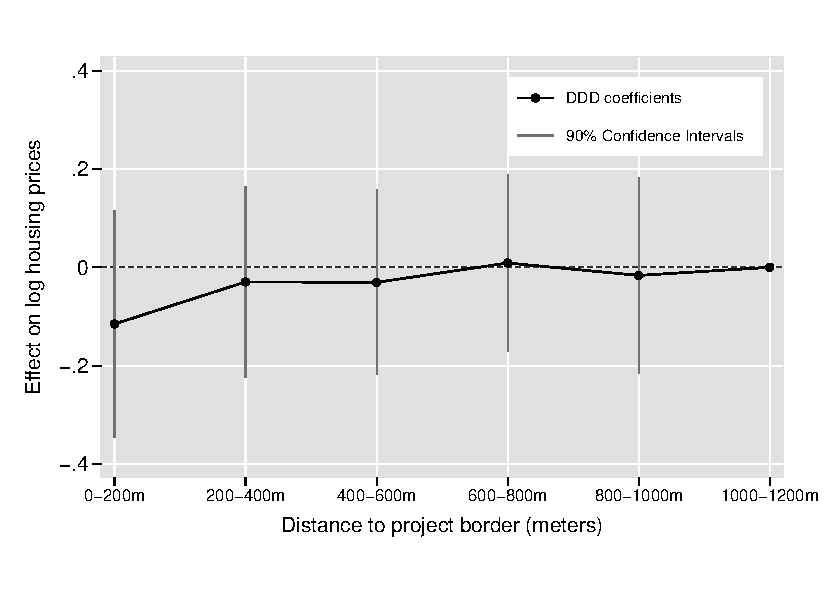
\includegraphics[width=0.9\textwidth,trim={0cm .7cm 0cm 0.7cm},clip=true]{figures/price_regs_DDDplot}
\vspace{-2mm}
\end{figure}

\begin{figure}[b!]
\caption{Price Estimates over Distance from Project Het}\label{figure:distplot_het}
\centering
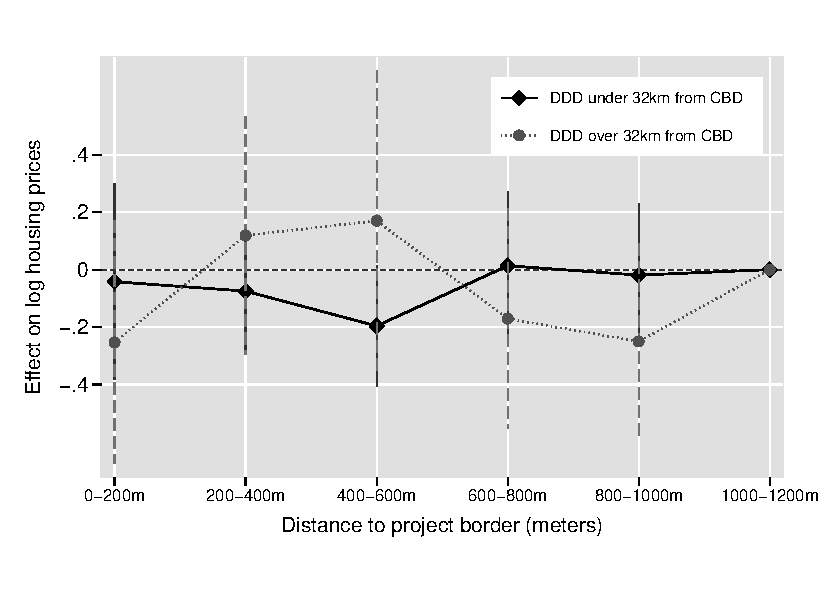
\includegraphics[width=0.9\textwidth,trim={0cm .7cm 0cm 0.7cm},clip=true]{figures/price_regs_DDDplot_het}
\vspace{-2mm}
\end{figure}


Figure~\ref{figure:distplot} plots coefficients $\alpha^d$ and associated standard errors for every $d\in D$. This specification includes project as well as calendar month fixed effects and includes only transactions that occur within three years of project construction.  Examining the point estimates, we find evidence of a drop in prices of around 0.1 log points or around 10\% within 200 meters of the project boundary.  Beyond 200 meters, this negative price effect disappears with all point estimates closely tracking zero.  Clustering standard errors at the project-level leaves wide confidence intervals at all distances, meaning that we are unable to reject equivalence between any coefficient and the price effect for the reference category at the 10\% confidence level.

Table~\ref{table:priceDDD} provides point estimates for distance bins up to 600 meters across a variety of controls and using a broader reference category including all distances from 600 meters to 1,200 meters.  The first row confirms a price drop of around 10\% that is relatively stable as we include additional controls for project, time, and location.  We find much smaller but similarly negative price effects between 200 and 600 meters.  Wide standard errors ensure that no coefficients are statistically different from zero. Due to the noisiness of the data, we are unable to rule out large effects at all distances. 

\begin{table}[h!]
\small
\centering
\caption{Triple Difference Estimates on Log-Prices}\label{table:priceDDD}
\vspace{-2mm}
\begin{tabular}{lCCCC}
\toprule
 & \small (1) & \small (2) & \small (3) & \small (4) \\ \midrule 
0 to 200m   &      -0.104&      -0.103&      -0.160&      -0.155\\
            &     (0.127)&     (0.093)&     (0.093)&     (0.118)\\[0.5em]
200m to 400m&      -0.061&      -0.058&      -0.111&      -0.104\\
            &     (0.099)&     (0.074)&     (0.084)&     (0.097)\\[0.5em]
400m to 600m&       0.057&       0.011&      -0.038&      -0.061\\
            &     (0.086)&     (0.077)&     (0.074)&     (0.073)\\ \midrule
Cubic in lot size&  \checkmark&  \checkmark&  \checkmark&  \checkmark\\
Project \textsc{FE}&           .&  \checkmark&           .&           .\\
Year{\tim}Project \textsc{FE}&           .&           .&  \checkmark&           .\\
Year{\tim}Lat-Lon cell \textsc{FE}&           .&           .&           .&  \checkmark\\
Year-Month \textsc{FE}&  \checkmark&  \checkmark&           .&           .\\
Month \textsc{FE}&           .&           .&  \checkmark&  \checkmark\\
R$^2$       &       0.174&       0.347&       0.381&       0.264\\
N           &     120,866&     120,866&     120,866&     120,866\\

\bottomrule
\multicolumn{5}{l}{\footnotesize Standard errors clustered at the project level in parenthesis. \textsuperscript{c} p$<$0.10,\textsuperscript{b} p$<$0.05,\textsuperscript{a} p$<$0.01 }
\end{tabular}
\end{table} 



\begin{table}[h!]
\small
\centering
\caption{Triple Difference Estimates on Log-Prices Het}\label{table:priceDDD_het}
\vspace{-2mm}
\begin{tabular}{lCCCC}
\toprule
 & \small (1) & \small (2) & \small (3) & \small (4) \\ \midrule 
Near CBD 0 to 200m&      -0.067&      -0.073&      -0.059&      -0.178\\
            &     (0.198)&     (0.197)&     (0.218)&     (0.201)\\[0.5em]
Near CBD 200m to 400m&      -0.093&      -0.105&      -0.100&      -0.206\\
            &     (0.162)&     (0.119)&     (0.122)&     (0.132)\\[0.5em]
Near CBD 400m to 600m&      -0.220&      -0.228&      -0.242&      -0.291\\
            &     (0.172)&     (0.125)&     (0.131)&     (0.125)\\[0.5em]
Far from CBD 0 to 200m&      -0.538&      -0.183&       0.020&      -0.413\\
            &     (0.252)&     (0.196)&     (0.223)&     (0.292)\\[0.5em]
Far from CBD 200m to 400m&      -0.179&       0.188&       0.306&       0.019\\
            &     (0.251)&     (0.191)&     (0.195)&     (0.130)\\[0.5em]
Far from CBD 400m to 600m&      -0.162&       0.248&       0.358&       0.043\\
            &     (0.264)&     (0.272)&     (0.250)&     (0.297)\\
Cubic in lot size&  \checkmark&  \checkmark&  \checkmark&  \checkmark\\
Project \textsc{FE}&           .&  \checkmark&           .&           .\\
Year{\tim}Project \textsc{FE}&           .&           .&  \checkmark&           .\\
Year{\tim}Lat-Lon cell \textsc{FE}&           .&           .&           .&  \checkmark\\
Year-Month \textsc{FE}&  \checkmark&  \checkmark&           .&           .\\
Month \textsc{FE}&           .&           .&  \checkmark&  \checkmark\\
R$^2$       &       0.202&       0.334&       0.356&       0.289\\
N           &      87,253&      87,253&      87,253&      87,253\\

\bottomrule
\multicolumn{5}{l}{\footnotesize Standard errors clustered at the project level in parenthesis. \textsuperscript{c} p$<$0.10,\textsuperscript{b} p$<$0.05,\textsuperscript{a} p$<$0.01 }
\end{tabular}
\end{table} 

\begin{figure}[t!]
\caption{Time-to-Event Price Estimates}\label{figure:timeplot}
\centering
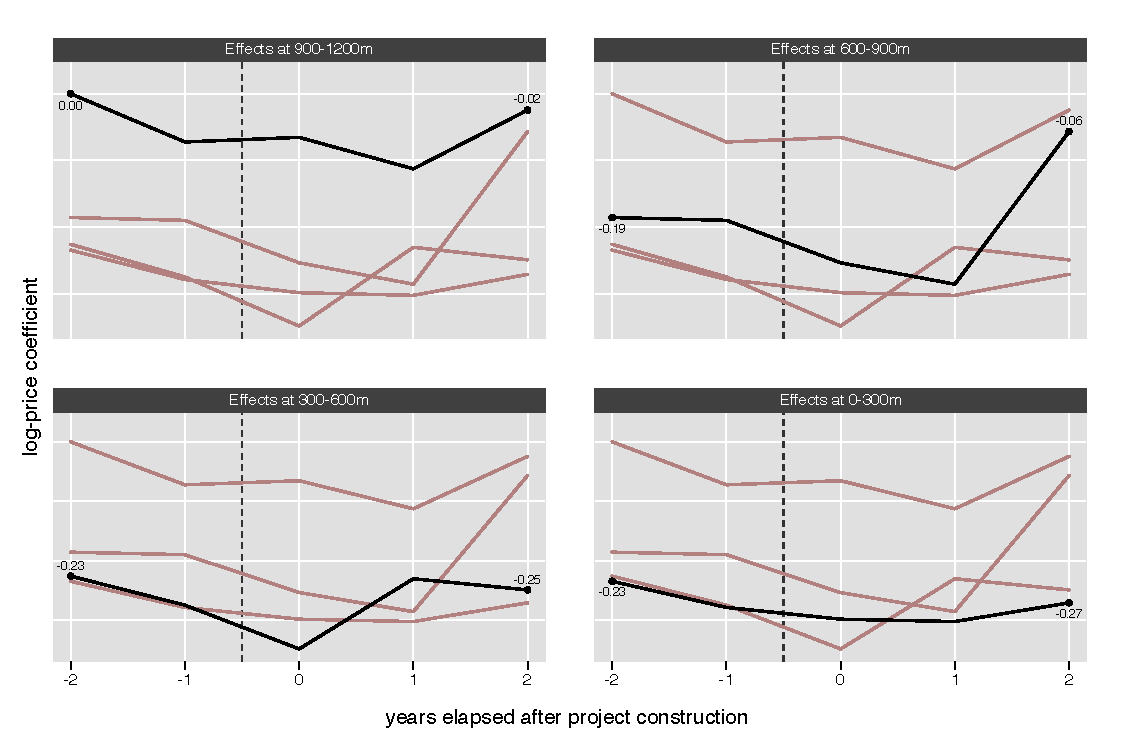
\includegraphics[width=0.99\textwidth,trim={0cm 0cm 0cm 0cm},clip=true]{figures/DDDplot_pertime_alt_unspaghetti}
\vspace{-2mm}
\end{figure}

We look into the dynamics of these effects by substituting the $\textsc{\small Post}_{pt}$ term with year dummies relative to the date of construction. We estimate these trends separately for four different distance bins relative to the project boundary.  Figure~\ref{figure:timeplot} plots these coefficients, excluding the confidence intervals.  Further splitting the sample for this exercise widens the confidence intervals so that all 90\% intervals contain zero.  We set the reference category to be two-years prior to project construction for the furthest distance bin. Figure~\ref{figure:timeplot} shows some evidence of anticipation, with prices level declining one year before construction at all distances. After project construction, prices appear to gradually recover. %Time trends for distances beyond 600 meters appear relatively uncorrelated with the time of project completion, suggesting that these areas may be unaffected by project construction.








\section{Conclusion}\label{section:discussion}

\begin{comment}

Our results present a puzzle: large improvements in housing quality and infrastructure access within projects do not appear to generate new investments in formal housing development, influxes of high-income residents, or increases in housing prices nearby these projects.  Additionally, we find no evidence that low-income households differentially sort into project areas or that projects increase the total supply of housing --- both mechanisms which may counteract any positive amenity effects.  We offer two partial explanations to account for this puzzle.

In making housing decisions, people in South Africa may simply have weak preferences for neighborhood quality.  Given very high rates of unemployment especially in rural areas, many South Africans migrate to cities solely for employment, sending large shares of their income home to their families.  In the census data, we observe that over 43\% of our sample reports being born outside the province of Gauteng.  Young adults regularly engage in circular migration, returning periodically to rural villages to spend their leisure time.  Rather than investing in the local community and developing a strong social network, people may view their housing decision in terms of short-term access to employment.  Therefore, people may place little value on nearby neighborhood quality or other amenities, instead prioritizing low rents and short commutes. 

Another explanation is that households value neighborhood quality, but higher densities of informal backyard shacks offset any improvements in formal housing quality and infrastructure.  \cite{Brueckner2018backyarding} document how households in backyard shacks often share water, electricity, and sanitation services with their landlords.  Congestion in using shared services may lead households to consume less of these services and exacerbate externalities associated with these low levels of usage.  \cite{Brueckner2018backyarding} also emphasize that backyard shacks often house young-adult, migrant workers who may be less inclined to make long-term social or economic investments in their communities.  

These results contrast with similar findings in both developed and developing country settings. - what papers to discuss?


Our interpretation is relatively neutral from a policy perspective: housing projects can produce enough positive amenities to mediate any housing supply effects.  Additionally, these projects effectively replace informal settlements with high quality formal houses, achieving a signature goal of South Africa's policy.  At the same time, there is little evidence supporting housing policy as an important engine for local economic growth and development.  These results may at least mediate any concerns policymakers may have for adversely affecting communities with housing projects, despite sometimes loud complaints from nearby community members.


It is important to emphasize that our analysis does not currently speak to the overall welfare implications of these policies.  Since project houses cannot be sold, we have difficulty measuring the extent to which households value these houses.  


Similarly, we do not measure the general equilibrium effects of housing policy outside of project neighborhoods; public housing may lead to an overall net reduction in slums in the city, which may generate total welfare gains through fewer congestion externalities or other mechanisms.  

In light of South Africa's emphasis on using housing policy to stimulate neighborhood development, we hope that this paper will be useful for policymakers in considering the range of informal housing market responses as they design new housing policies.

% We find that South African housing projects greatly improve the housing conditions within their footprints.  Housing projects successfully deliver large numbers of new formal structures (Figure~\ref{figure:dddformal}) and much better access to bulk services (Table~\ref{table:censusestimates}).  At the same time, formal project housing appears to crowd-out growth in informal settlements so that the total density of housing remains the same as in unconstructed project areas (Figure~\ref{figure:dddtotal}).  Moreover, results in Table~\ref{table:censusestimates} indicate that the average quality of new project houses are at least as good as neighboring houses at baseline.  Therefore consistent with the model of amenity effects in \cite{diamond2016wants}, we would expect to find that these programs increase nearby home prices; however, results in Table~\ref{table:priceest} report if anything the opposite trend.  Similarly, we do not observe large new developments in either informal or formal housing just nearby these projects.

% The lack of significant spillover effects in price as well as in quantity is consistent with countervailing amenity and housing supply effects.  While an influx of new houses threatens to decrease prices and housing supply nearby, positive amenities provided by housing projects may also attract greater housing investment, increasing prices.  While both amenity and supply effects predict increases in local population, there may be spatial or geographic constraints on population growth given that these settlements in South Africa are almost exclusively single-story and informal settlements often fill any remaining surface area.


%\section{Conclusion}\label{section:conclusion}
%This paper serves as a cautionary tale for low-density public housing in developing countries.  While these projects may be designed to improve local housing markets and reduce local slum growth, they may instead support local slum growth through a mix of available land and improved infrastructure.  It is important to emphasize that our analysis does not currently speak to the overall welfare implications of these policies.  For example, public housing may lead to an overall net reduction in slums in the city, which may generate total welfare gains through fewer congestion externalities or other mechanisms.  According to our model, the optimal housing policy depends crucially on the shape of these congestion externalities.  We look forward to using variation in the South African housing program to estimate these externalities in future work.  


% (1) construction costs, (2) value to recipients, (3) value to non-recipients within project footprints, and (4) spillover effects on neighboring areas.  


\end{comment}


\pagebreak

\nocite{*}
\singlespacing
\setlength{\bibsep}{7pt}
\bibliographystyle{abbrvnat}
\bibliography{ref}



\pagebreak
% APPENDIX 
\appendix
\doublespacing

\section{Appendix}

\titleformat*{\subsection}{\centering\normalsize\bfseries}


\begin{figure}[t]
\caption{Transaction Price Histogram}\label{figure:transactionhist}
\centering
\tcbox[colback=white,boxrule=.35mm,boxsep=0mm]{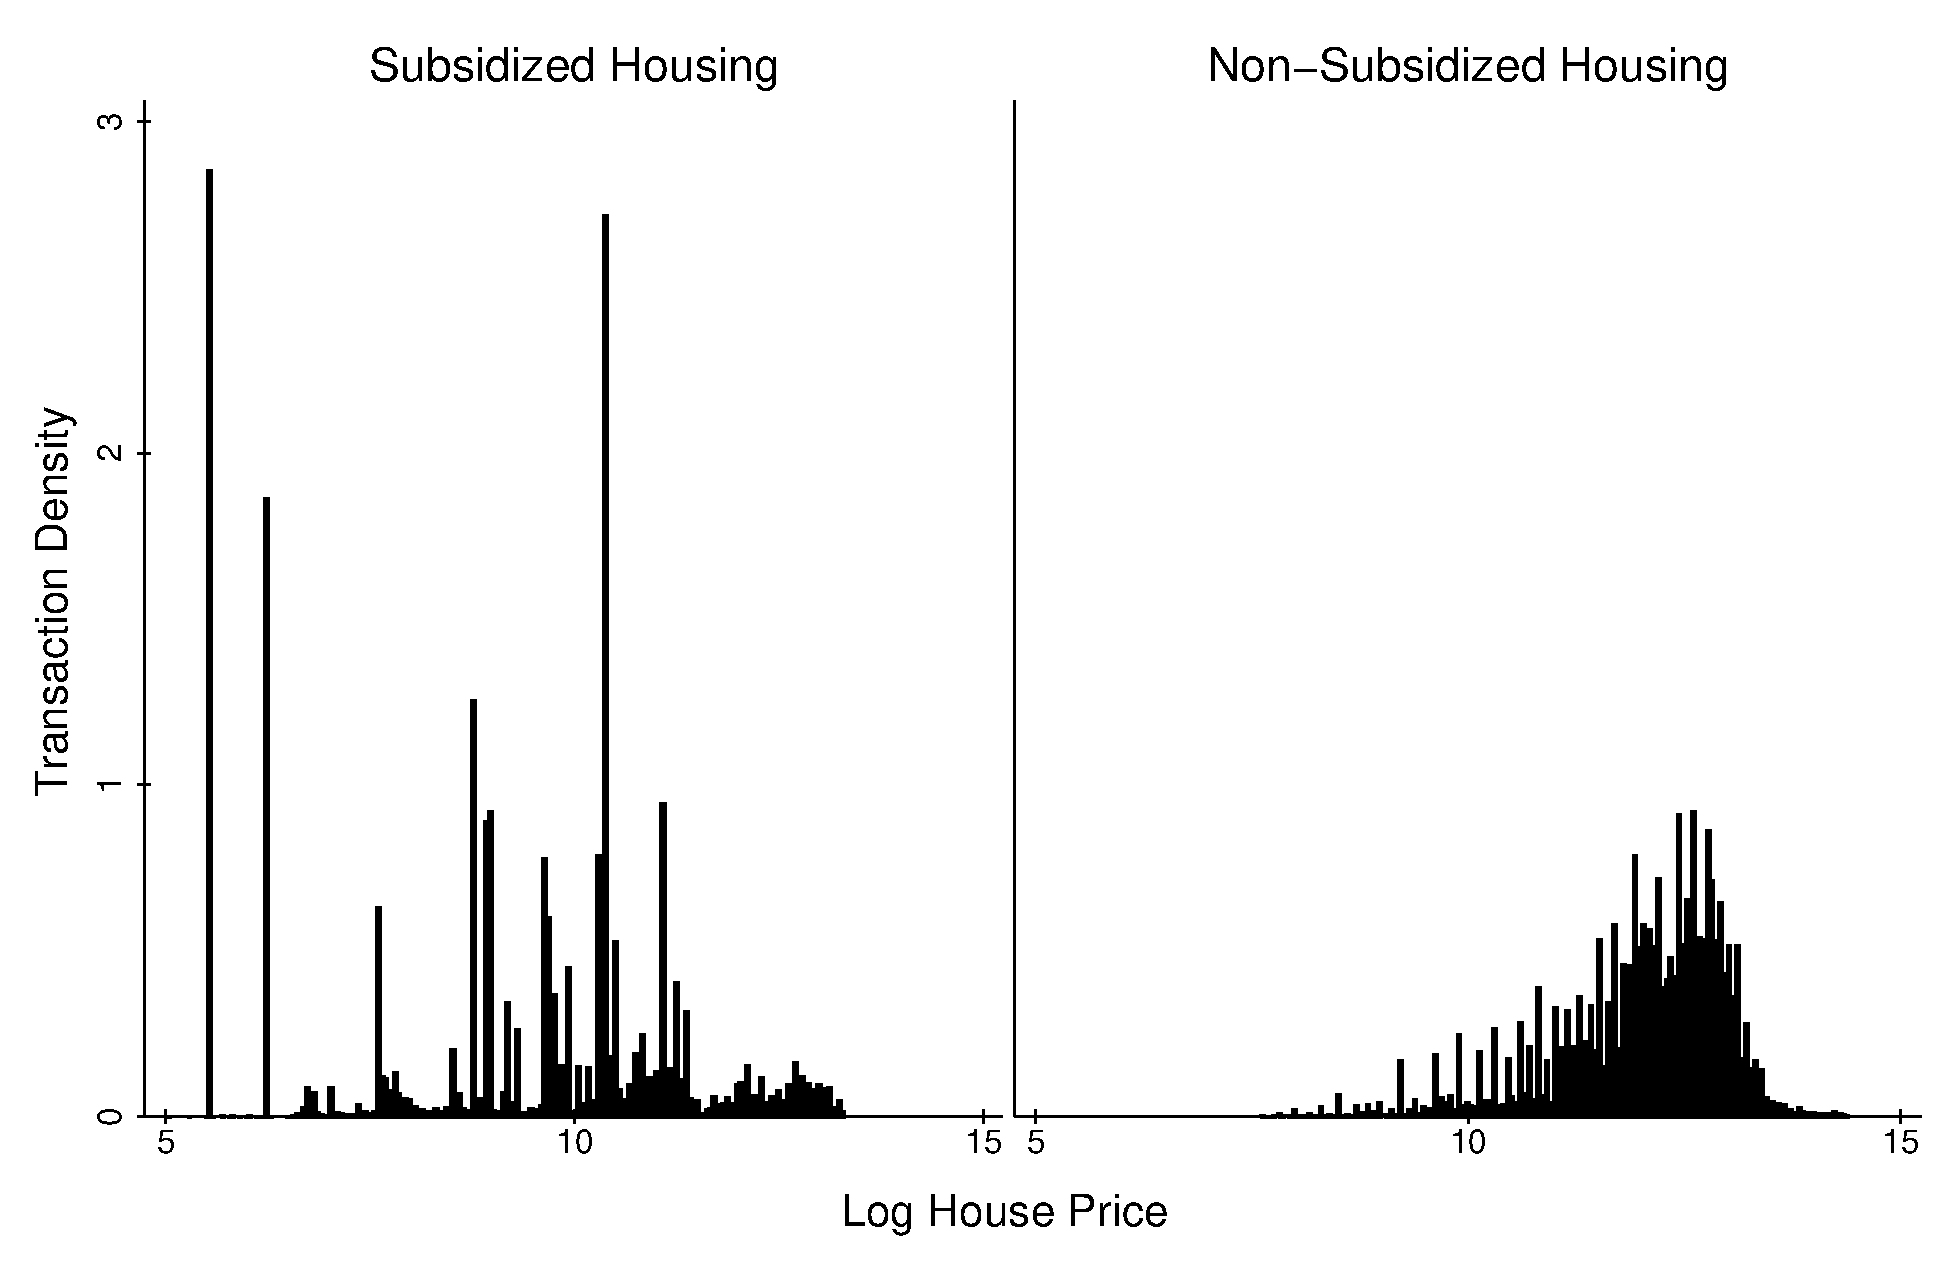
\includegraphics[scale=.4,trim={0cm 0cm -1cm 0cm}]{figures/summary_pricedist.pdf}}
%\\
%\footnotesize{Note: Transactions are censored at R100,000.}
\end{figure}


\subsection{Project Descriptions}\label{appendix:projectdescriptions}

\begin{table}[h!]
\centering
\caption{Project Descriptions}\label{table:projectdescriptions}
\vspace{-2mm}
\begin{tabular}{l*{1}{c}}
\toprule
 &Counts  \\
\midrule
\textbf{Constructed} & \\[.5em]
current  & 89 \\current/overflow  & 24 \\under implementation  & 45 \\complete  & 14 \\[.5em]
Total constructed  & 172 \\[.5em]
\textbf{Unconstructed} & \\[.5em]
proposed  & 71 \\under planning  & 40 \\future  & 16 \\investigating  & 10 \\uncertain  & 8 \\[.5em]
Total unconstructed  & 145 \\[.5em]
\textbf{Other} \\[.5em]
informal  & 87 \\hostel  & 23 \\new  & 27 \\upg  & 6 \\p  & 1 \\no description  & 181 \\[.5em]
Total other  & 325 \\[.5em]
\midrule
Total  & 642 \\[.5em]
\bottomrule
\end{tabular}
\end{table}



\subsection{String Matching for Project Names and Delivery Dates }
\label{appendix:stringmatch}

%\begin{center}
%[...]
%\end{center}



%\begin{comment}

We then use a fuzzy-string matching algorithm with bigrams to link project names from the budget reports to the administrative maps.  We keep all matches with over 60\% similarity, with 37 projects matching exactly.  Appendix~\ref{table:stringmatch} compares unmatched and matched projects finding that matched projects have much higher numbers of project houses, lower nearby housing prices, and are further from the central business district compared to unmatched projects.  One reason may be that the budget reports only include larger, more expansive projects, which are likely to take place further from city centers. 

% We find that the project start date (from the budget reports) is three years before the project completion date (from the deeds data) on average.  In other words, beneficiaries receive title to their new houses about three years after the housing program is announced in the budget.  Using this lag, we assign an expected completion date for unconstructed projects that is three years after the announced start-date in the budget reports.  Since the budget data does not include month of planning, we assign a random month for unconstructed projects, which ensures that this date is uncorrelated with seasonality but also introduces measurement error in the timing of unconstructed projects.  This error is only likely to affect the housing transaction estimates, which are the only estimates performed at the monthly level.  

% \begin{table}
% 	\centering
% 	\caption{Assessing Name Matching between \\Budget and Spatial Administrative Data}\label{table:stringmatch}
% \begin{tabu}{lcc}
 & Matched  & Unmatched  \\
\midrule
 Formal Density: 2001  & 230.5  & 171.5  \\ 
 Formal Density: 2011  & 814.1  & 444.0  \\ 
 &  &  \\ 
 Informal Density: 2001  & 1,055.6  & 1,401.0  \\ 
 Informal Density: 2011  & 1,613.2  & 2,147.0  \\ 
 &  &  \\ 
 Project House Density  & 125.0  & 66.0  \\ 
 Project Mode Year  & 2005  & 2005  \\ 
 &  &  \\ 
 Hectares  & 97.3  & 119.6  \\ 
 &  &  \\ 
\midrule
 Observations  & 322  & 320  \\ 
\bottomrule
\end{tabu}
 \\
% Density is measured in structures per $\text{km}^{2}$.
% \end{table}
% %\end{comment}

\vspace{0mm}
\begin{table}
\centering
\caption{Assessing Name Matching between Budget Reports and the Administrative Map}\label{table:stringmatch}
\vspace{0mm}
\begin{tabular}{l*{1}{cccc}}
\toprule
  & \multicolumn{2}{c}{\textbf{Matched}}& \multicolumn{2}{c}{\textbf{Unmatched}}    \\
  &Const. & Unconst. &Const. & Unconst.  \\
\midrule
 Number of Projects  & 126  & 73  & 46  & 72  \\ 
 Area (km2)  & 1.22  & 1.02  & 1.05  & 1.30  \\ 
 Delivered Houses  & 416  & 15  & 259  & 7  \\ 
 House Price in 1 km (R$^\dagger$)  & 183,930  & 206,496  & 199,923  & 232,166  \\ 
 Distance to CBD$^\ddagger$ (km)  & 34.3  & 31.3  & 27.5  & 24.0  \\ 

\bottomrule
\multicolumn{5}{l}{\scriptsize Const. refers to constructed projects and unconst. refers to unconstructed projects.}\\[-.5em]
\multicolumn{5}{l}{\scriptsize $^*$Calculated from {\it expected} completion dates using Gauteng National Treasury budget reports.}\\[-.5em]
\multicolumn{5}{l}{\scriptsize $^\dagger$ The USD averaged to about 7.70 Rands during the 2001-2011 period.}\\[-.5em]
\multicolumn{5}{l}{\scriptsize $^\ddagger$Measured as the average minimum distance with respect to Johannesburg and Pretoria CBDs. } \\[-.5em]
\end{tabular}
\end{table} 


\subsection{Buffer Design for Census small-areas}
\label{appendix:bufferdesign}

\vspace{-3mm}

\begin{figure}[h!]
%\caption{Buffer Design for Census small-areas}\label{figure:bufferdesigncensus}
\centering
\tcbox[colback=white,boxrule=.35mm,boxsep=0mm]{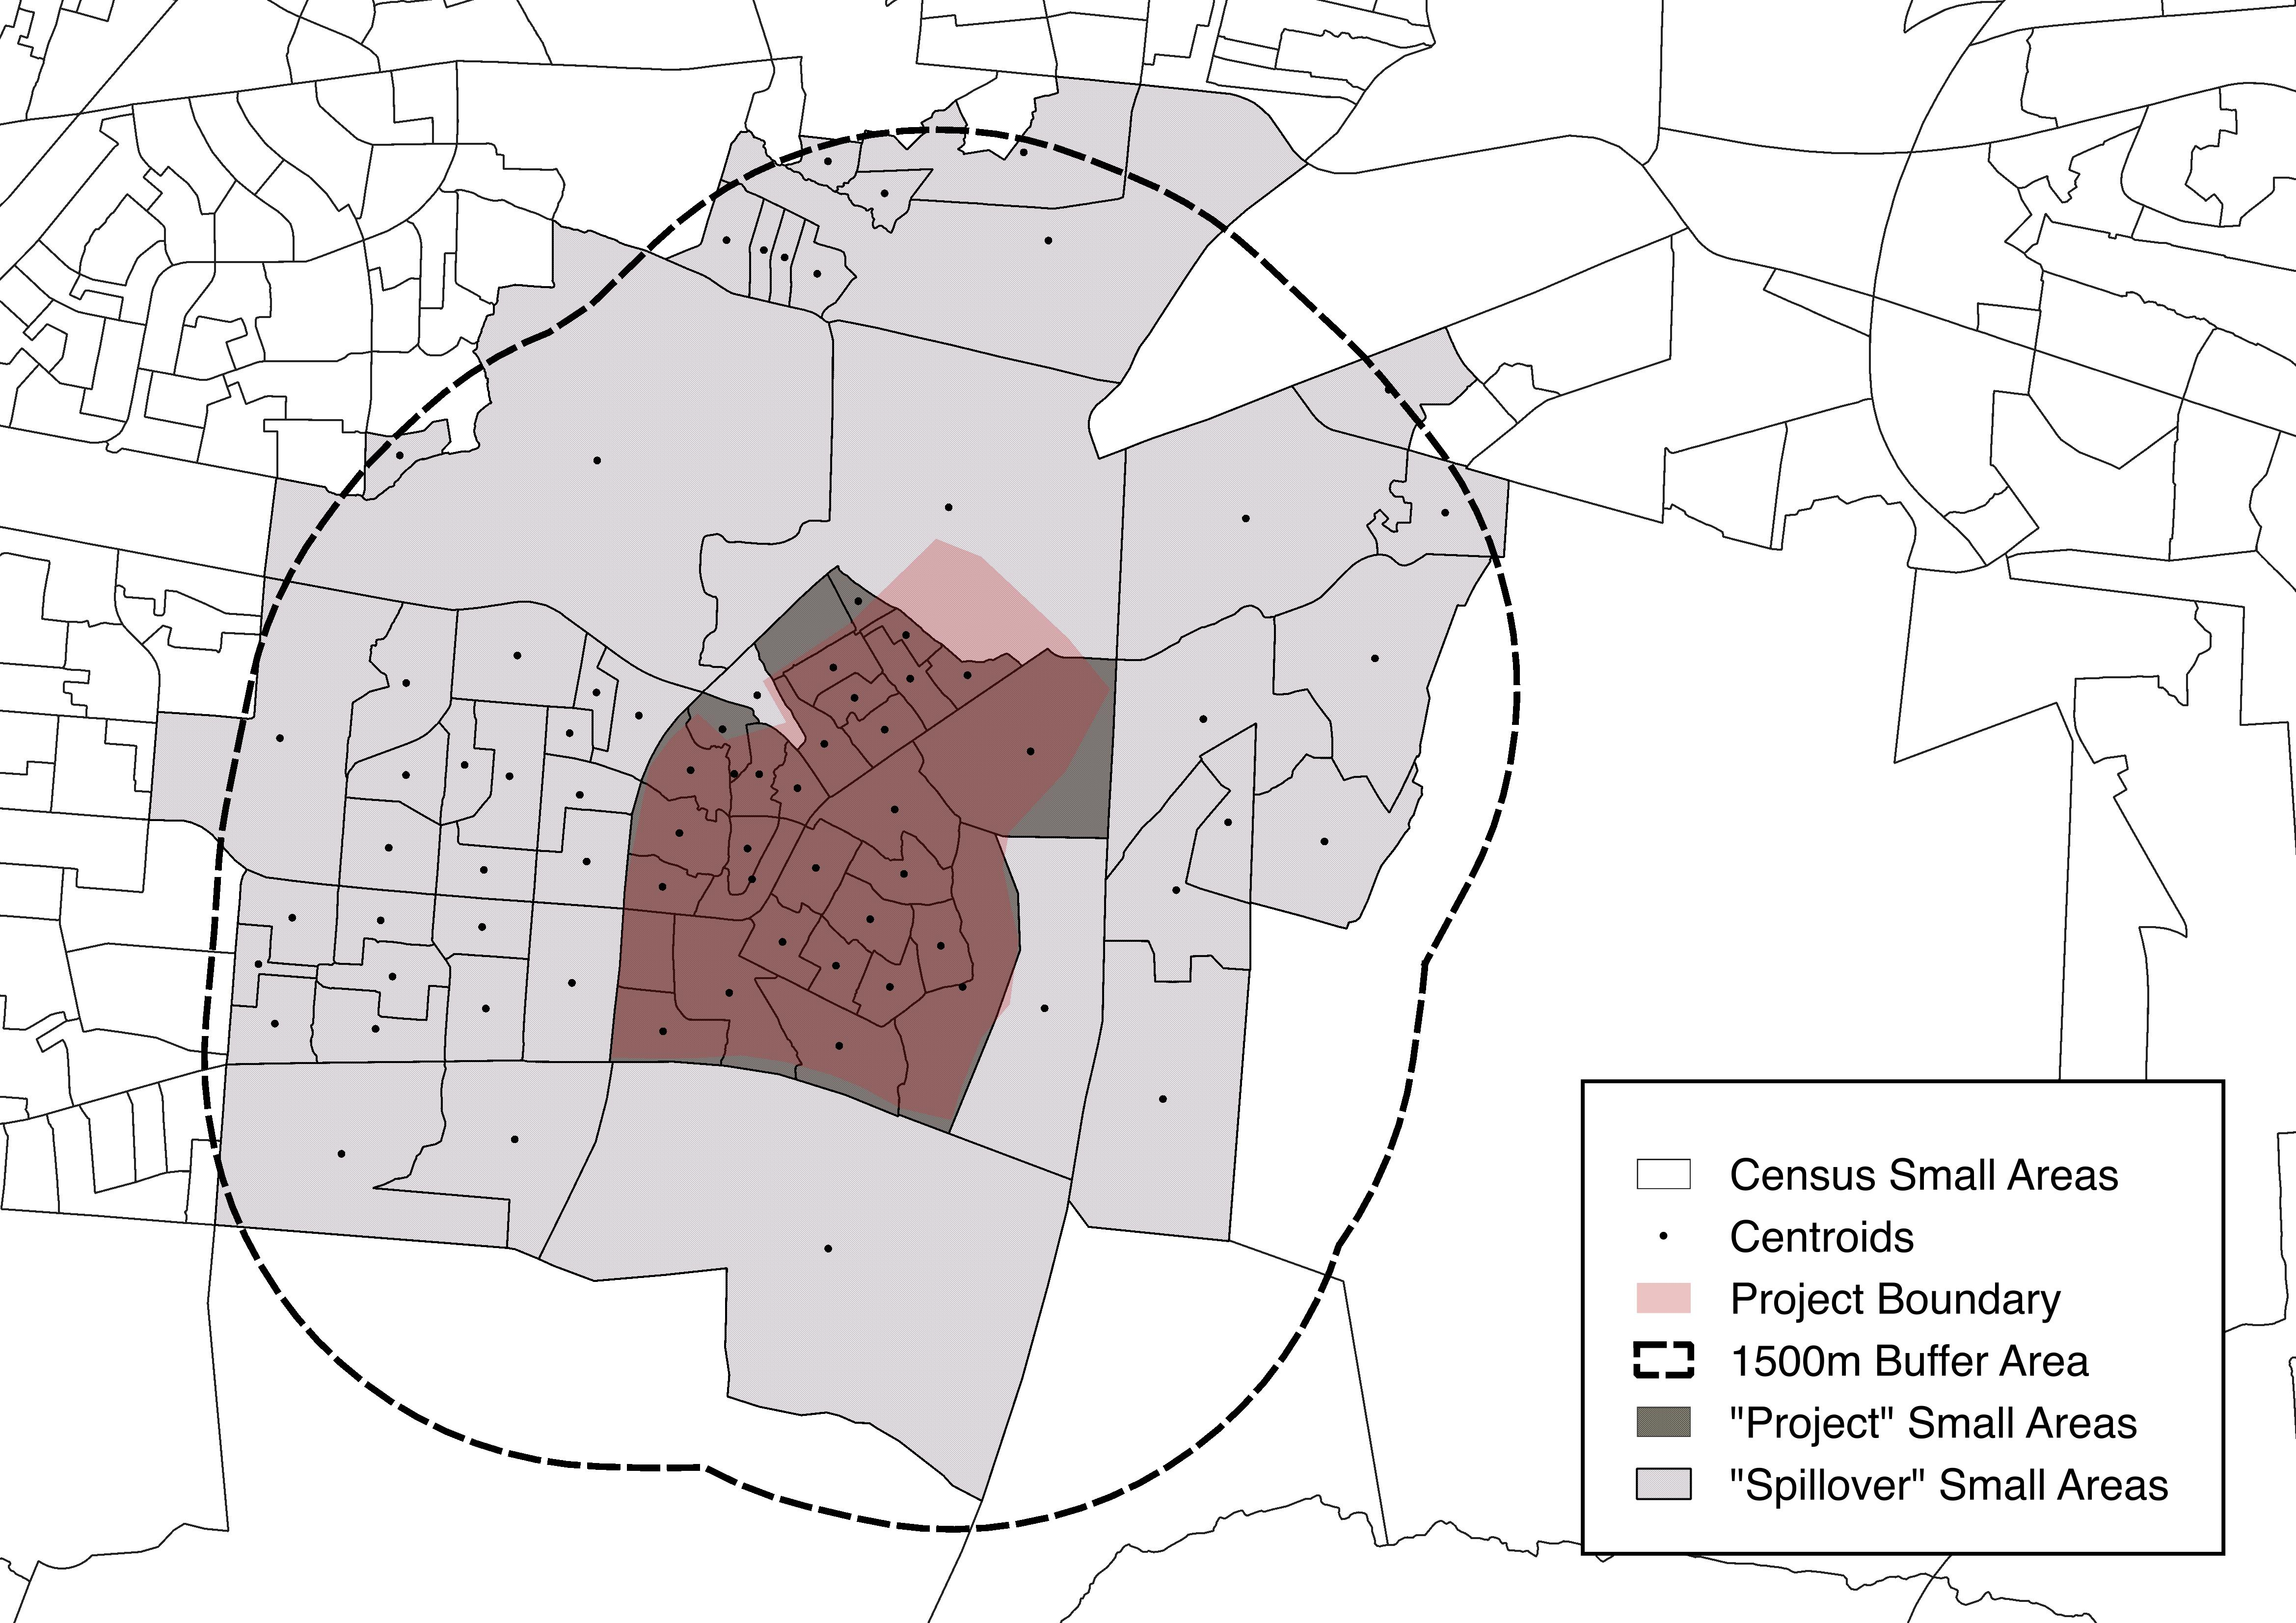
\includegraphics[scale=.47,trim={.75cm .4cm .75cm .4cm}]{figures/census_design.jpg}}
\vspace{2mm}
\caption*{\footnotesize {\bf Note:} We consider every census small-areas whose centroid fall within 1500m of a project boundary. We denote small-areas with over 30\% area overlap with project boundaries as "project" small-areas, and use household responses within these geographies to capture dwelling characteristics inside project boundaries. All remaining small-areas are denoted as "spillover" geographies, and are used to capture dwelling characteristics nearby.}
\end{figure}

\pagebreak
\subsection{Transaction Frequency}
\label{appendix:histfreq}
\vspace{-5mm}
\begin{figure}[h!]
\centering
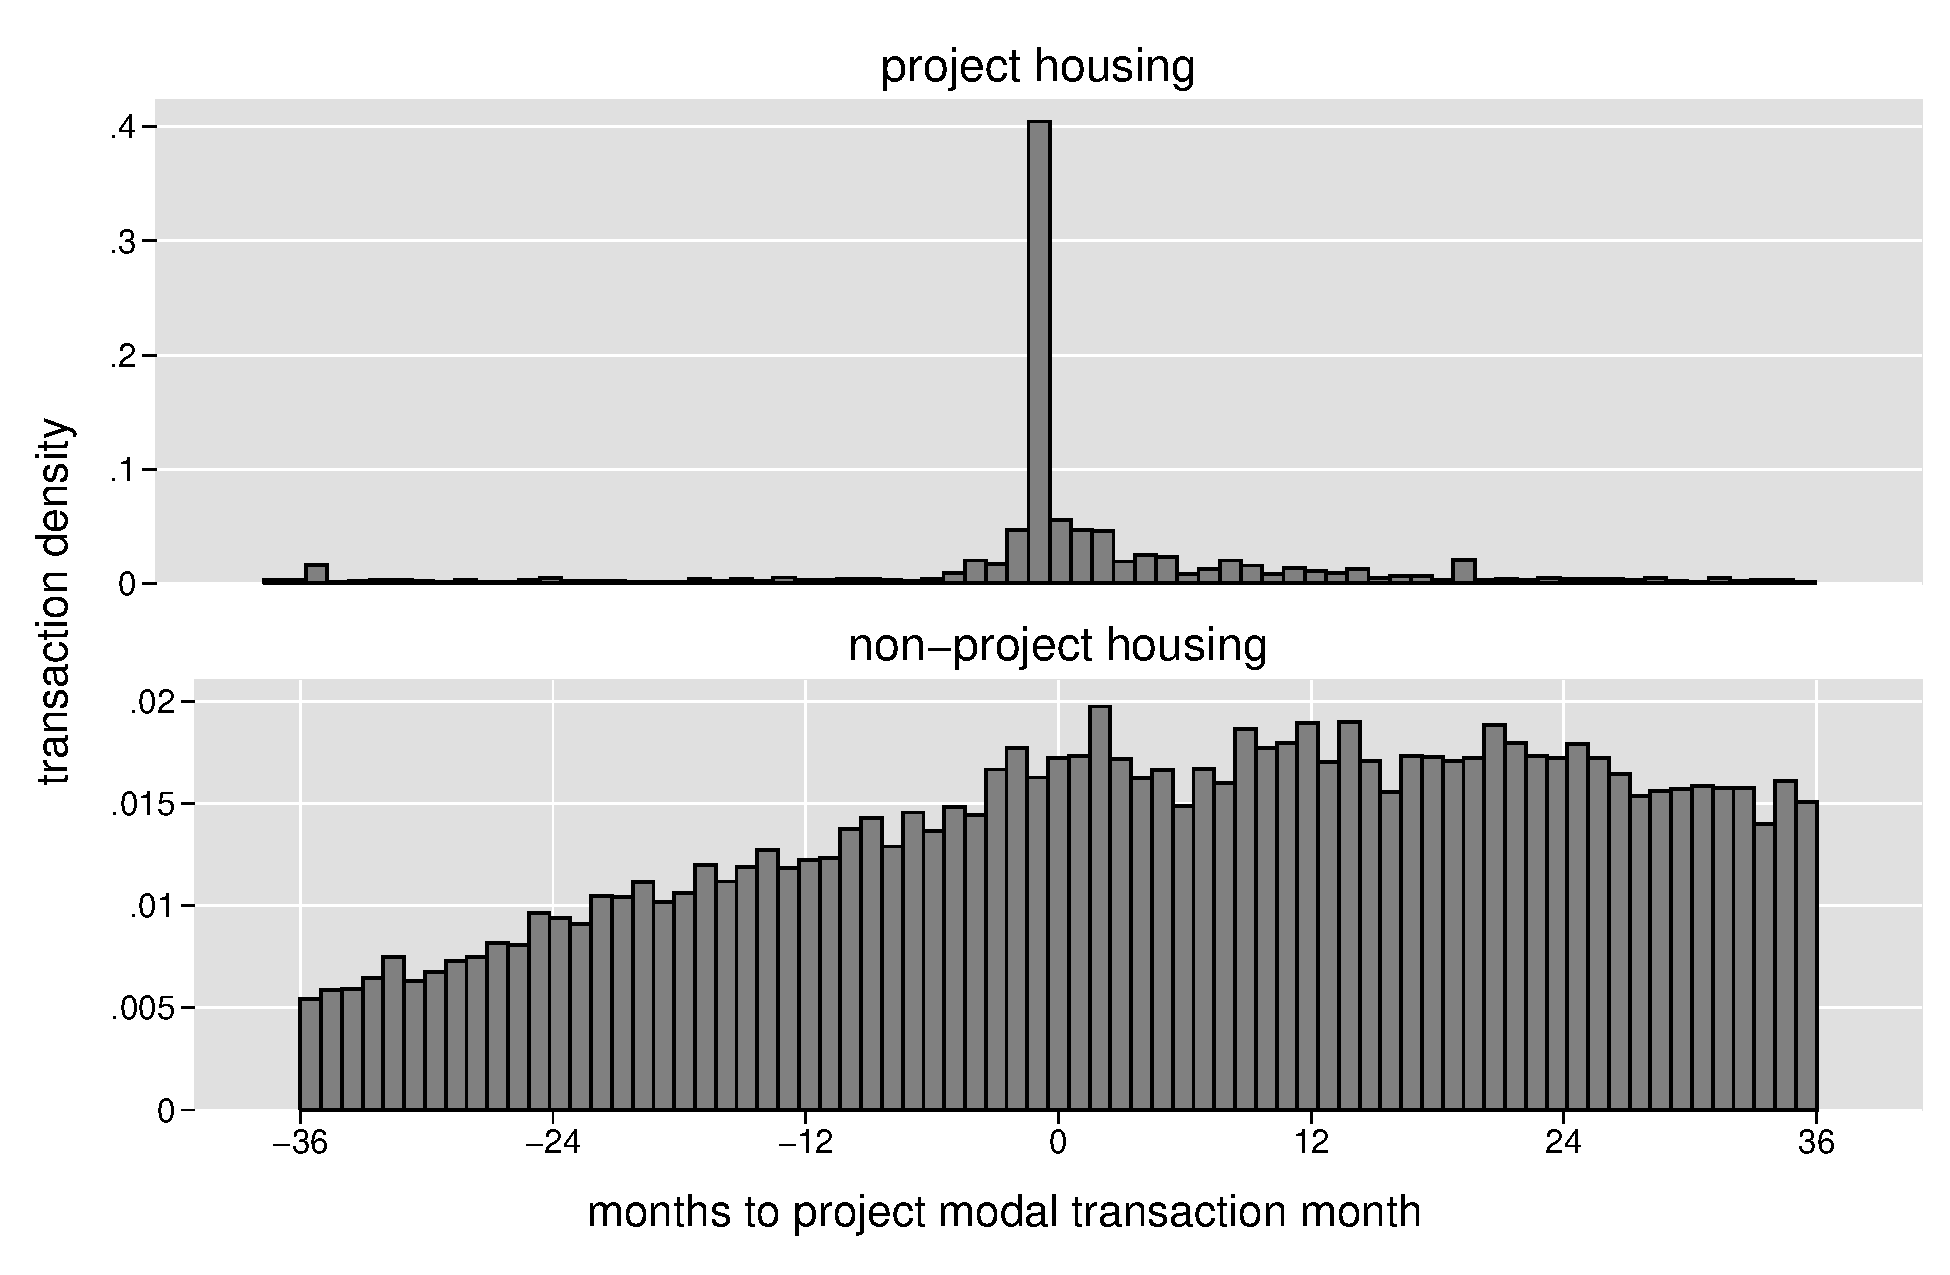
\includegraphics[scale=.4 , trim={.2cm 0.2cm .2cm 0.2cm},clip]{figures/summary_densitytime.pdf}
\end{figure}

\pagebreak
\subsection{Project counts}
\label{appendix:projectcounts}
\vspace{-5mm}
\begin{figure}[h!]
\centering
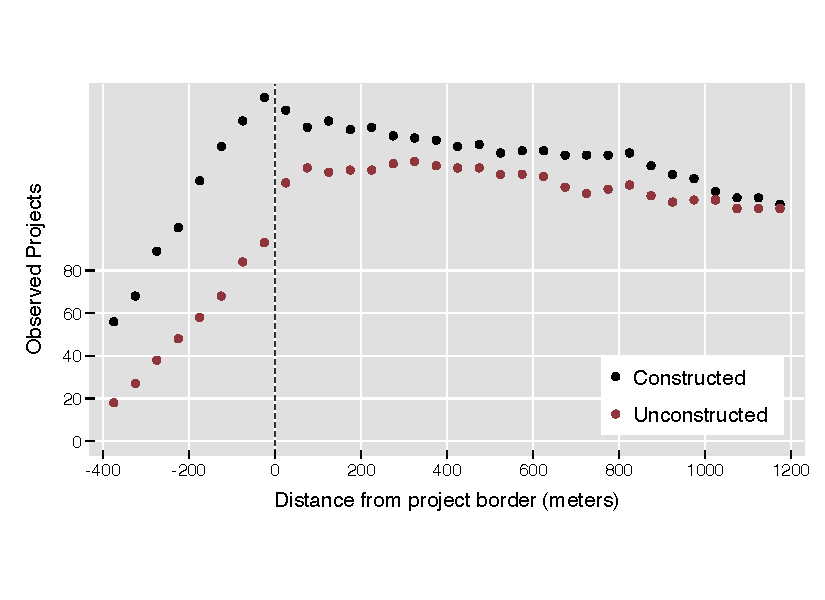
\includegraphics[scale=1.2,trim={.1cm 1.2cm .1cm 1.2cm},clip]{figures/projectcounts_4.pdf}
\end{figure}



\begin{table}[h!]
	\centering
	\caption{Dwelling Characteristics at Baseline from 2001 Census: City versus Suburb}\label{table:projectdescriptivescensushet}
\vspace{-2mm}
\begin{tabular}{l*{1}{ccccc}}
\toprule
& \multicolumn{2}{c}{\textbf{City}} & \multicolumn{2}{c}{\textbf{Suburb}} &   \\
& Const. & Unconst. & Const. & Unconst. &  All  \\
\midrule
Flush Toilet&0.66&0.41&0.45&0.56&0.81 \\
Piped Water in Home&0.16&0.12&0.07&0.29&0.47 \\
Electricity for Cooking&0.34&0.28&0.30&0.49&0.73 \\
Electricity for Heating&0.31&0.28&0.27&0.46&0.70 \\
Electricity for Lighting&0.54&0.31&0.63&0.64&0.82 \\
Number of Rooms&2.42&2.23&3.25&2.90&3.72 \\
Household Size&3.30&3.06&3.74&3.42&3.32 \\
N&            445&            135&            479&            151&         10,711 \\
 
\bottomrule
\multicolumn{6}{l}{\scriptsize ``Const.'' and ``Unconst.'' include census small-areas with over 30\% }  \\ [-.5em]
\multicolumn{6}{l}{\scriptsize  area overlap with constructed and unconstructed projects respectively. } \\ [-.5em]
\multicolumn{6}{l}{\scriptsize ``All''  includes all small-areas.  ``City'' includes areas within 30.4 km } \\ [-.5em]
\multicolumn{6}{l}{\scriptsize of a CBD and ``Suburb'' includes areas over 30.4 km away from a CBD. } 
\end{tabular}
\end{table}



\vspace{0mm}
\begin{table}[h!]
\centering
\caption{Housing Project Areas Description}\label{table:projectdescriptives_het}
\vspace{0mm}
\begin{tabular}{l*{1}{cccccc}}
\toprule
  & \multicolumn{2}{c}{\textbf{All}}& \multicolumn{2}{c}{\textbf{Greenfield}}  & \multicolumn{2}{c}{\textbf{In-Situ Upgrading}}   \\
  &Const. & Unconst. &Const. & Unconst.   & Const. & Unconst. \\
\midrule
 Number of Projects  & 172  & 145  & 43  & 20  & 27  & 29  \\ 
 Area (km2)  & 1.17  & 1.16  & 1.72  & 2.42  & 1.50  & 0.88  \\ 
 Median Construction Yr.  & 2006  & 2006  & 2006  & 2005  & 2004  & 2006  \\ 
 Delivered Houses  & 374  & 11  & 568  & 24  & 702  & 20  \\ 
 House Price in 1 km (R$^\dagger$)  & 188,441  & 218,635  & 194,214  & 186,841  & 179,596  & 208,570  \\ 
 Distance to CBD$^\ddagger$ (km)  & 32.5  & 27.7  & 40.5  & 39.9  & 32.6  & 30.6  \\ 

\bottomrule
\multicolumn{7}{l}{\scriptsize Const. refers to constructed projects and unconst. refers to unconstructed projects.}\\[-.5em]
\multicolumn{7}{l}{\scriptsize $^*$Calculated from {\it expected} completion dates using Gauteng National Treasury budget reports.}\\[-.5em]
\multicolumn{7}{l}{\scriptsize $^\dagger$ The USD averaged to about 7.70 Rands during the 2001-2011 period.}\\[-.5em]
\multicolumn{7}{l}{\scriptsize $^\ddagger$Measured as the average minimum distance with respect to Johannesburg and Pretoria CBDs. } \\[-.5em]
\end{tabular}
\end{table} 



\begin{table}
\caption{Building Density Heterogeneity by Project Type}
\begin{tabular}{lDDDDD}
\toprule
 & \small (1) & \small (2)  & \small (3) & \small (4) & \small (5) \\
 & Total & Formal  & Informal & Informal Bkyd. & Informal Non-Bkyd. \\
  \midrule
\textbf{Greenfield} \\   inside project      &     300.851                   &     171.702                   &     129.149                   &      87.898                   &      41.251                   \\
                    &   (349.583)                   &   (289.394)                   &   (106.795)                   &   (194.841)                   &   (144.318)                   \\[0.01em]
0-500m outside project &    -105.918                   &     -76.529                   &     -29.389                   &    -113.755                   &      84.366                   \\
                    &   (235.140)                   &   (107.801)                   &   (144.512)                   &   (112.770)                   &    (85.988)                   \\[0.8em] 
\textbf{In-Situ Upgrading} \\   inside project      &    1439.960\textsuperscript{b}&    1193.277\textsuperscript{a}&     246.684                   &    1168.161\textsuperscript{a}&    -921.478\textsuperscript{b}\\
                    &   (578.606)                   &   (196.043)                   &   (484.009)                   &   (292.300)                   &   (435.532)                   \\[0.01em]
0-500m outside project &    -200.201                   &     126.071                   &    -326.273                   &      46.457                   &    -372.729\textsuperscript{c}\\
                    &   (268.022)                   &   (137.120)                   &   (236.728)                   &   (162.396)                   &   (217.809)                   \\[0.8em]
\textbf{Other} \\   inside project      &     992.993\textsuperscript{a}&     835.990\textsuperscript{a}&     157.003                   &     707.527\textsuperscript{a}&    -550.524\textsuperscript{a}\\
                    &   (243.992)                   &   (103.474)                   &   (191.455)                   &   (151.698)                   &   (150.363)                   \\[0.01em]
0-500m outside project &     -78.348                   &      -4.187                   &     -74.161                   &     -67.165                   &      -6.996                   \\
                    &   (175.377)                   &    (66.771)                   &   (141.681)                   &    (95.335)                   &   (102.451)                   \\[0.8em]
Mean Outcome 2001   &      524.85                   &      261.16                   &      263.69                   &       96.38                   &      167.31                   \\
Mean Outcome 2011   &      836.05                   &      384.05                   &      452.00                   &      286.03                   &      165.98                   \\
R$^2$               &       0.308                   &       0.278                   &       0.265                   &       0.194                   &       0.261                   \\
N                   &   6,822,716                   &   6,822,716                   &   6,822,716                   &   6,822,716                   &   6,822,716                   \\

\bottomrule
\end{tabular}
\end{table}






\begin{figure*}
        \centering
        \caption[ Pre-period housing densities in constructed and unconstructed projects by project type ]
       {\small Pre-period housing densities in constructed and unconstructed projects by project type } 
        \vspace{2mm}
        
        \begin{subfigure}[b]{0.48\textwidth}
                    \caption[Network2]%
            {{\footnotesize \textbf{Greenfield} pre-period formal  raw data}}    
            \label{fig:prefor}
            \centering
            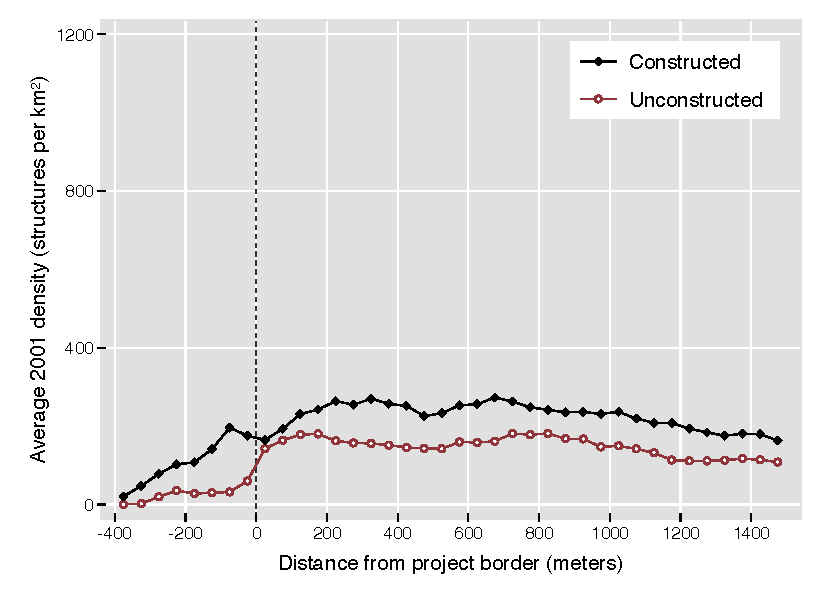
\includegraphics[width=\textwidth,trim={0.3cm .3cm 0.1cm 0cm}, clip=true]{figures/bblu_for_pre_means_4_1_spk.pdf}

        \end{subfigure}
        \hfill
        \begin{subfigure}[b]{0.48\textwidth}  
                    \caption[]%
            {{\footnotesize \textbf{Greenfield} pre-period informal  raw data}}     
            \label{fig:preinf}
            \centering 
            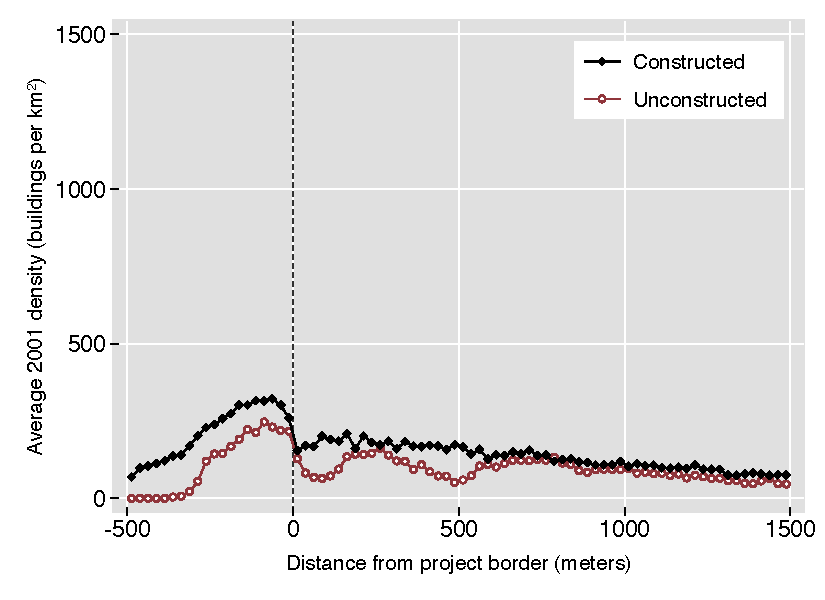
\includegraphics[width=\textwidth,trim={0.3cm .3cm 0.1cm 0cm}, clip=true]{figures/bblu_inf_pre_means_4_1_spk.pdf}

        \end{subfigure}
        \begin{subfigure}[b]{0.48\textwidth}
                    \caption[Network2]%
            {{\footnotesize \textbf{In-Situ} pre-period formal  raw data}}   
            \label{fig:prefor}
            \centering
            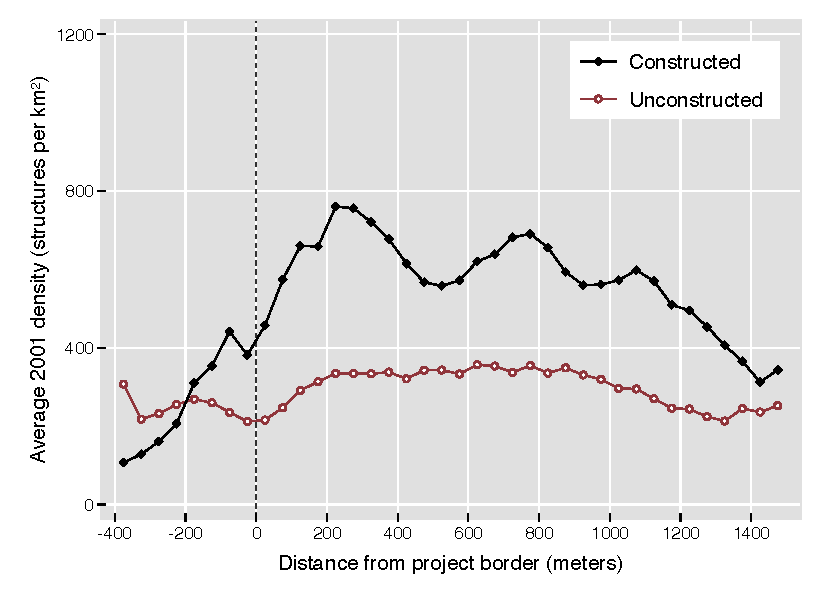
\includegraphics[width=\textwidth,trim={0.3cm .3cm 0.1cm 0cm}, clip=true]{figures/bblu_for_pre_means_4_2_spk.pdf}

        \end{subfigure}
        \hfill
        \begin{subfigure}[b]{0.48\textwidth}  
                    \caption[]%
            {{\footnotesize \textbf{In-Situ} pre-period informal  raw data}}     
            \label{fig:preinf}
            \centering 
            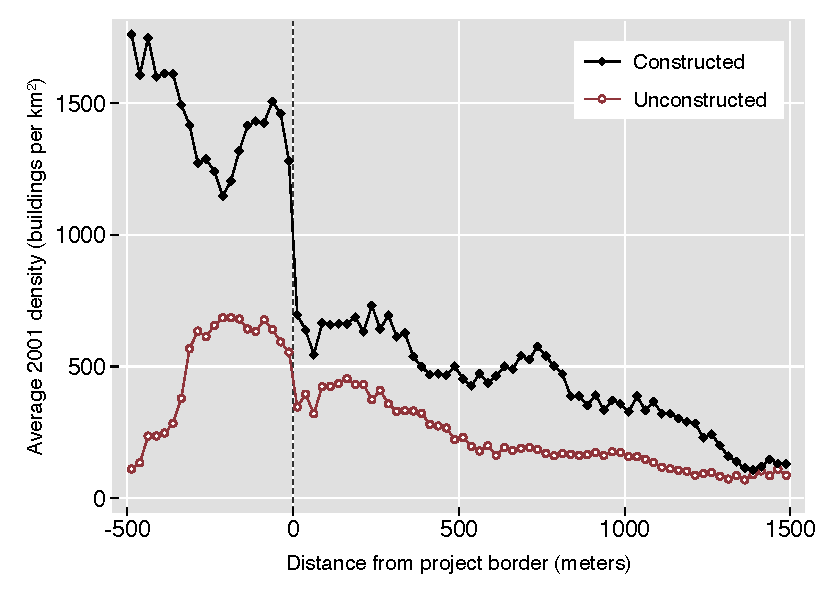
\includegraphics[width=\textwidth,trim={0.3cm .3cm 0.1cm 0cm}, clip=true]{figures/bblu_inf_pre_means_4_2_spk.pdf}

        \end{subfigure}
        \begin{subfigure}[b]{0.48\textwidth}
                    \caption[Network2]%
            {{\footnotesize \textbf{Other} pre-period formal  raw data}}   
            \label{fig:prefor}
            \centering
            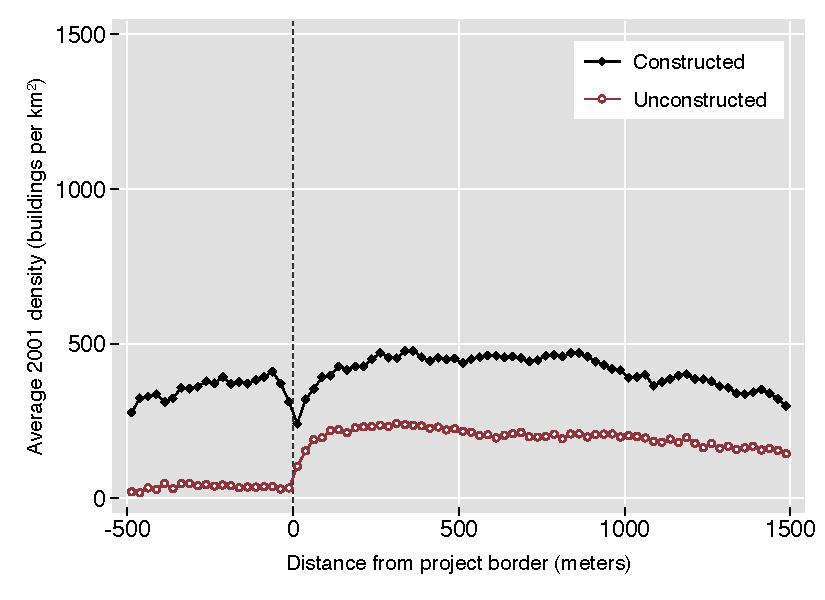
\includegraphics[width=\textwidth,trim={0.3cm .3cm 0.1cm 0cm}, clip=true]{figures/bblu_for_pre_means_4_3_spk.pdf}

        \end{subfigure}
        \hfill
        \begin{subfigure}[b]{0.48\textwidth}  
                    \caption[]%
            {{\footnotesize \textbf{Other} pre-period informal  raw data}}      
            \label{fig:preinf}
            \centering 
            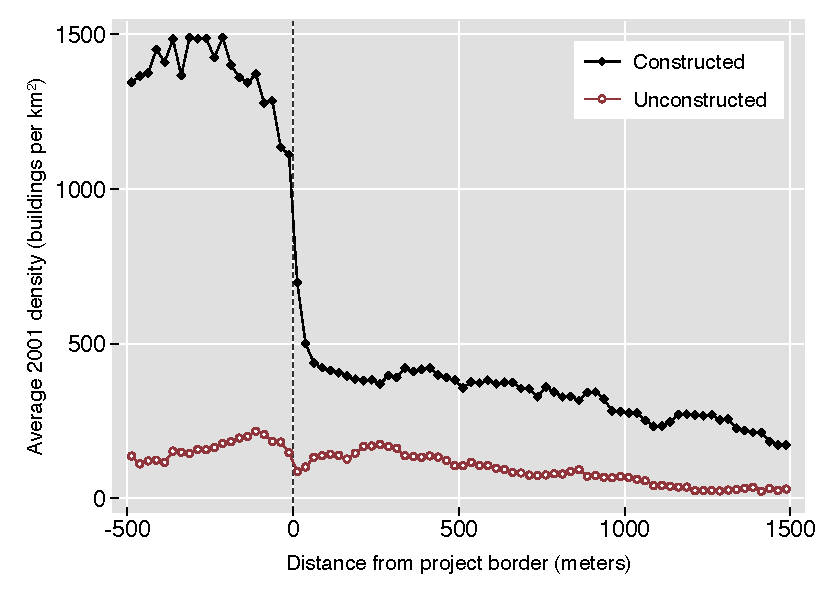
\includegraphics[width=\textwidth,trim={0.3cm .3cm 0.1cm 0cm}, clip=true]{figures/bblu_inf_pre_means_4_3_spk.pdf}

        \end{subfigure}
\end{figure*}




\begin{figure*}
        \centering
        \caption[ Pre-period housing densities for constructed and unconstructed projects by project type demeaned by 2001 census subplace]
        {\small Pre-period housing densities for constructed and unconstructed projects by project type demeaned by 2001 census subplace} 
        \vspace{2mm}
        \begin{subfigure}[b]{0.48\textwidth}
                    \caption[Network2]%
            {{\footnotesize \textbf{Greenfield} pre-period formal  fe }}    
            \label{fig:prefor}
            \centering
            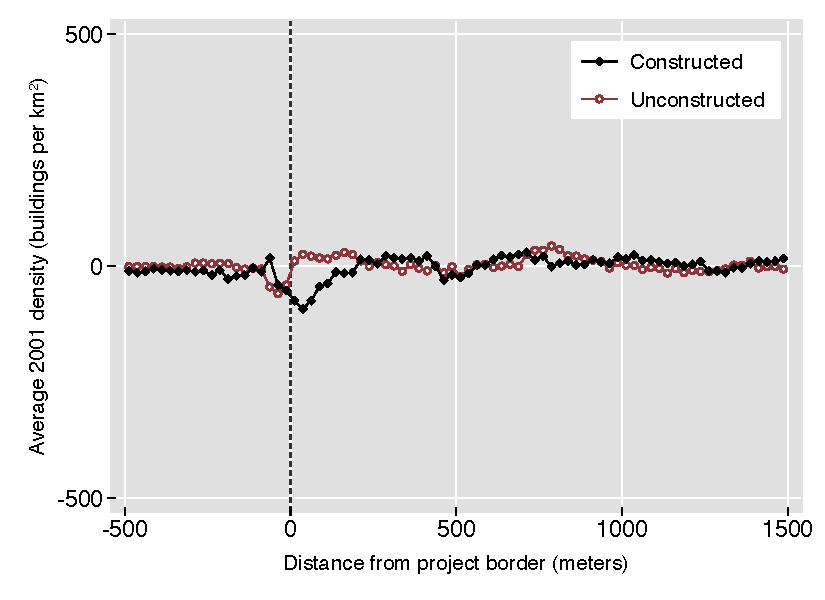
\includegraphics[width=\textwidth,trim={0.3cm .3cm 0.1cm 0cm}, clip=true]{figures/bblu_for_fe_pre_pre_means_4_1_spk.pdf}
        \end{subfigure}
        \hfill
        \begin{subfigure}[b]{0.48\textwidth}  
                    \caption[]%
            {{\footnotesize \textbf{Greenfield} pre-period informal fe }}     
            \label{fig:preinf}
            \centering 
            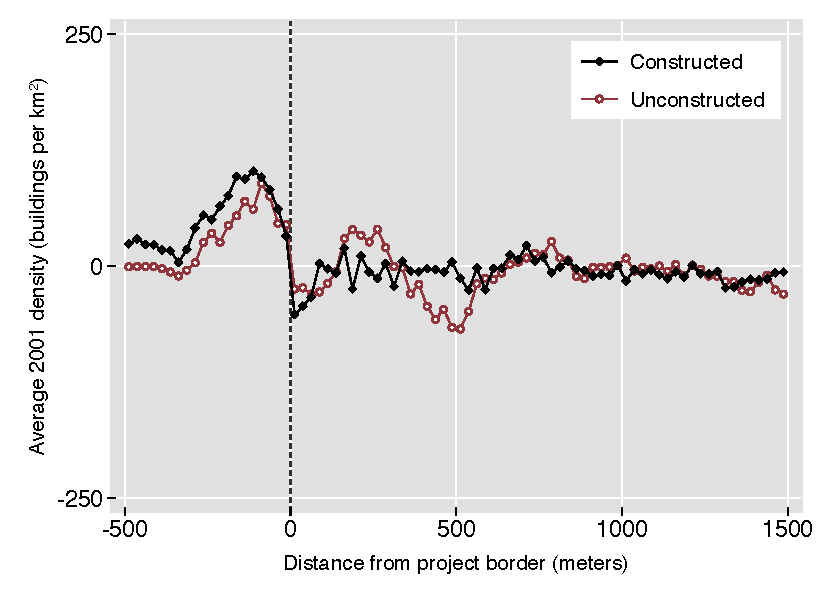
\includegraphics[width=\textwidth,trim={0.3cm .3cm 0.1cm 0cm}, clip=true]{figures/bblu_inf_fe_pre_pre_means_4_1_spk.pdf}

        \end{subfigure}
        \begin{subfigure}[b]{0.48\textwidth}
                    \caption[Network2]%
            {{\footnotesize \textbf{In-Situ} pre-period formal fe }}   
            \label{fig:prefor}
            \centering
            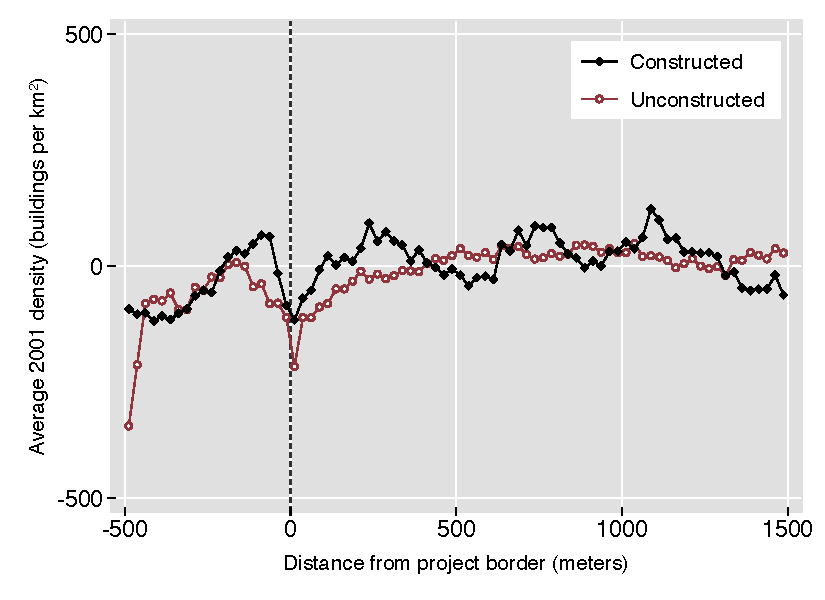
\includegraphics[width=\textwidth,trim={0.3cm .3cm 0.1cm 0cm}, clip=true]{figures/bblu_for_fe_pre_pre_means_4_2_spk.pdf}

        \end{subfigure}
        \hfill
        \begin{subfigure}[b]{0.48\textwidth}  
                    \caption[]%
            {{\footnotesize \textbf{In-Situ} pre-period informal fe }}     
            \label{fig:preinf}
            \centering 
            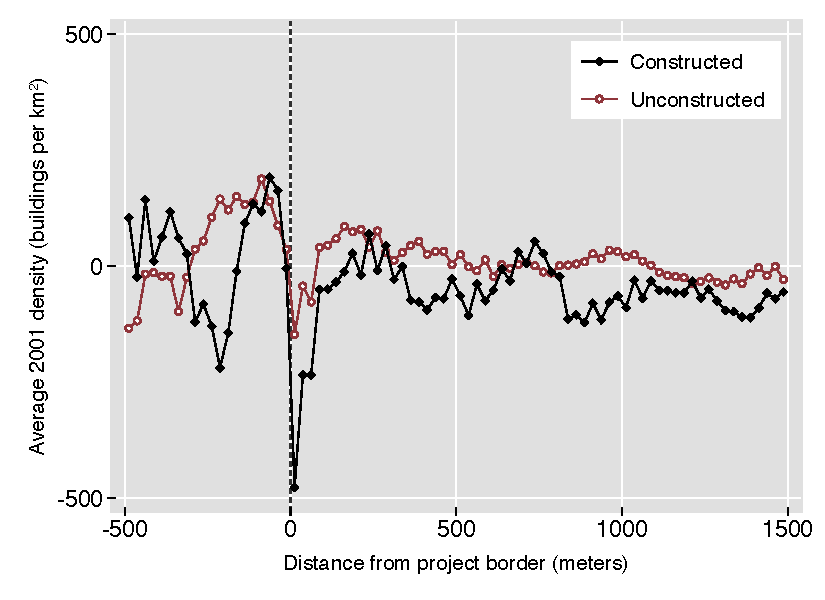
\includegraphics[width=\textwidth,trim={0.3cm .3cm 0.1cm 0cm}, clip=true]{figures/bblu_inf_fe_pre_pre_means_4_2_spk.pdf}

        \end{subfigure}
        \begin{subfigure}[b]{0.48\textwidth}
                    \caption[Network2]%
            {{\footnotesize \textbf{Other} pre-period formal fe }}   
            \label{fig:prefor}
            \centering
            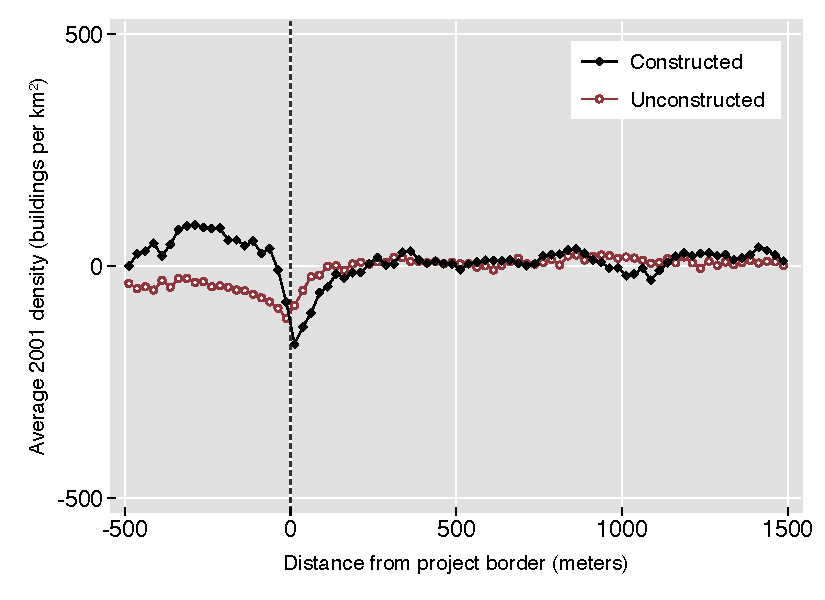
\includegraphics[width=\textwidth,trim={0.3cm .3cm 0.1cm 0cm}, clip=true]{figures/bblu_for_fe_pre_pre_means_4_3_spk.pdf}

        \end{subfigure}
        \hfill
        \begin{subfigure}[b]{0.48\textwidth}  
                    \caption[]%
            {{\footnotesize \textbf{Other} pre-period informal fe }}      
            \label{fig:preinf}
            \centering 
            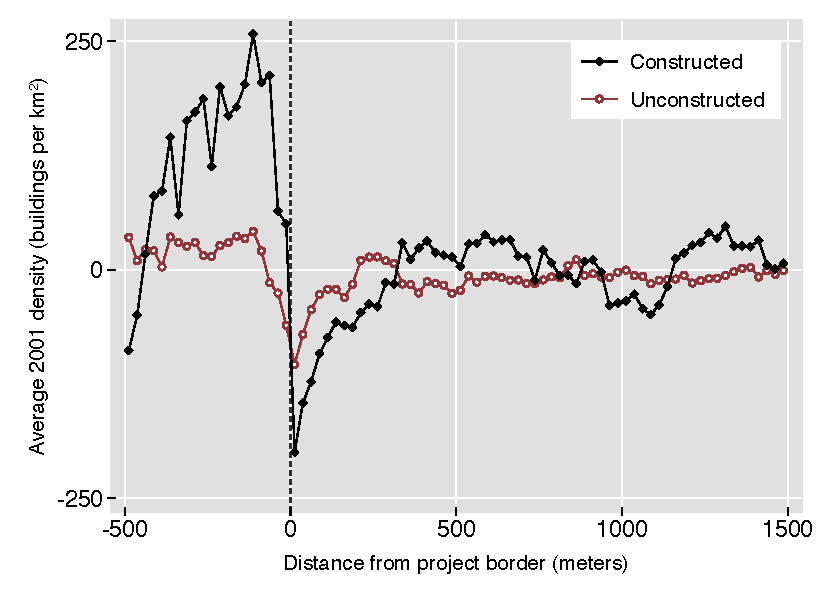
\includegraphics[width=\textwidth,trim={0.3cm .3cm 0.1cm 0cm}, clip=true]{figures/bblu_inf_fe_pre_pre_means_4_3_spk.pdf}

        \end{subfigure}
\end{figure*}




\begin{figure*}
        \centering
   %     \caption[ Pre-Period Housing Densities in Constructed and Unconstructed Projects Areas ]
  %      {\small Pre-Period Densities} 
        %\vspace{2mm}
       
        \begin{subfigure}[b]{0.48\textwidth}
                    \caption[Network2]%
            {{\footnotesize \textbf{Greenfield} changes formal  raw data}}    
            \label{fig:prefor}
            \centering
            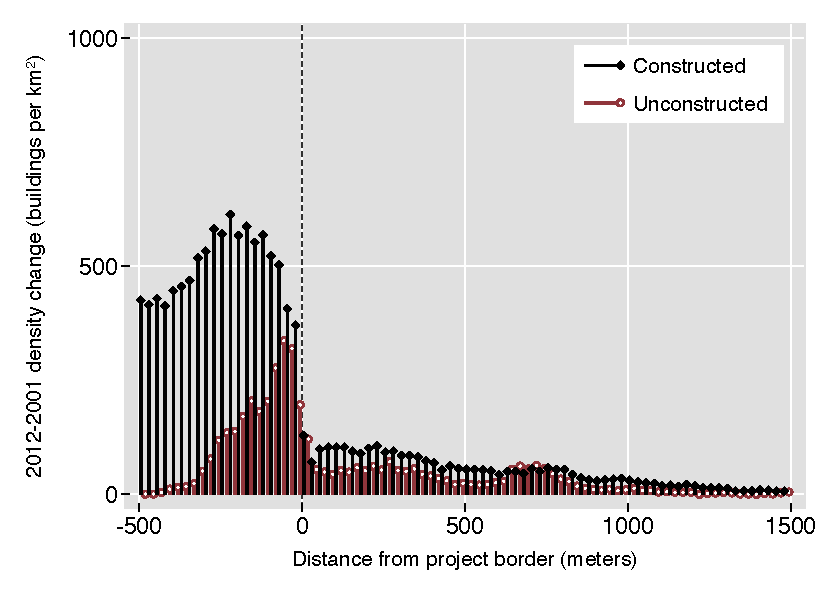
\includegraphics[width=\textwidth,trim={0.3cm .3cm 0.1cm 0cm}, clip=true]{figures/bblu_for_rawchanges_4_1_spk.pdf}

        \end{subfigure}
        \hfill
        \begin{subfigure}[b]{0.48\textwidth}  
                    \caption[]%
            {{\footnotesize \textbf{Greenfield} changes informal raw data }}     
            \label{fig:preinf}
            \centering 
            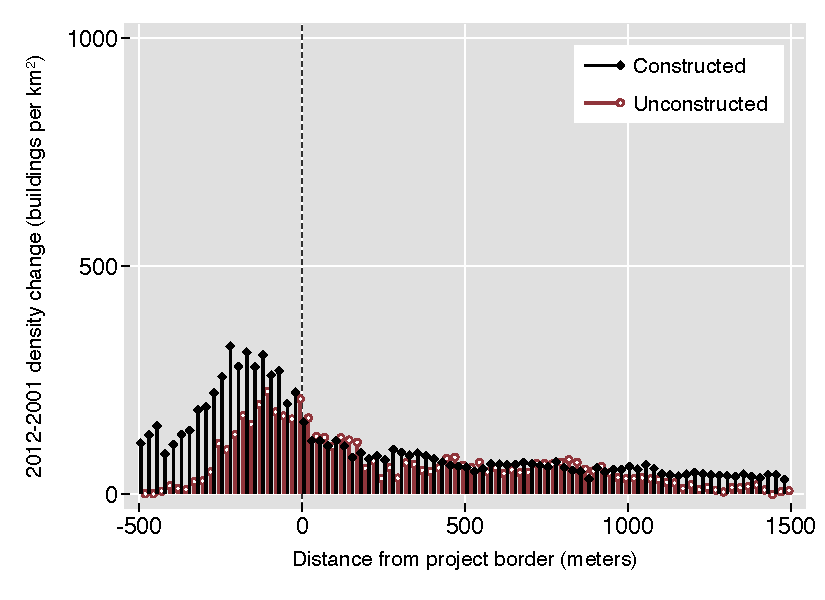
\includegraphics[width=\textwidth,trim={0.3cm .3cm 0.1cm 0cm}, clip=true]{figures/bblu_inf_rawchanges_4_1_spk.pdf}

        \end{subfigure}
        \begin{subfigure}[b]{0.48\textwidth}
                    \caption[Network2]%
            {{\footnotesize \textbf{In-Situ} changes formal raw data }}   
            \label{fig:prefor}
            \centering
            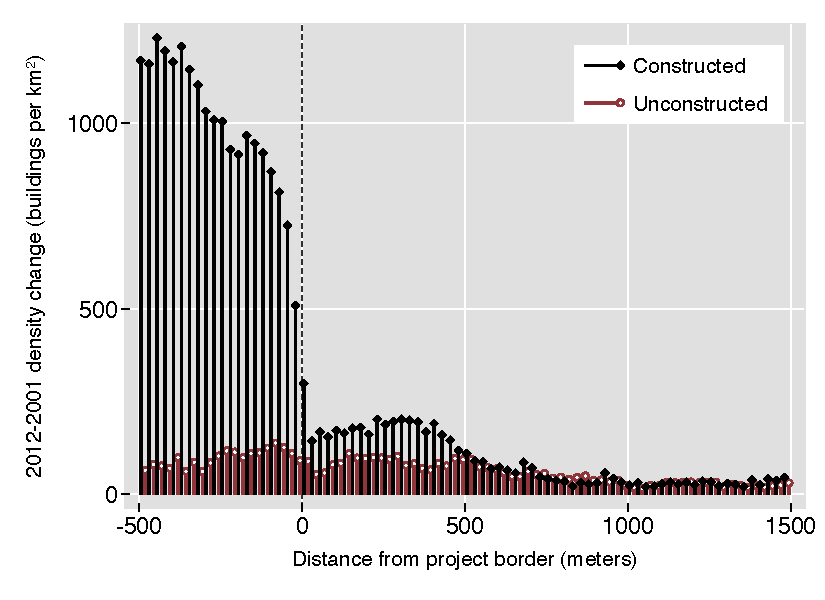
\includegraphics[width=\textwidth,trim={0.3cm .3cm 0.1cm 0cm}, clip=true]{figures/bblu_for_rawchanges_4_2_spk.pdf}

        \end{subfigure}
        \hfill
        \begin{subfigure}[b]{0.48\textwidth}  
                    \caption[]%
            {{\footnotesize \textbf{In-Situ} changes informal raw data }}     
            \label{fig:preinf}
            \centering 
            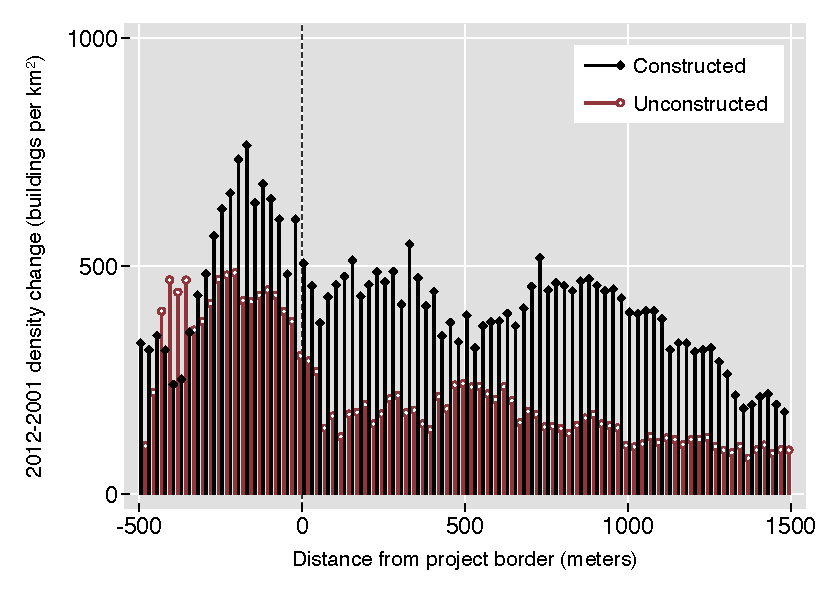
\includegraphics[width=\textwidth,trim={0.3cm .3cm 0.1cm 0cm}, clip=true]{figures/bblu_inf_rawchanges_4_2_spk.pdf}

        \end{subfigure}
        \begin{subfigure}[b]{0.48\textwidth}
                    \caption[Network2]%
            {{\footnotesize \textbf{Other} changes formal raw data}}   
            \label{fig:prefor}
            \centering
            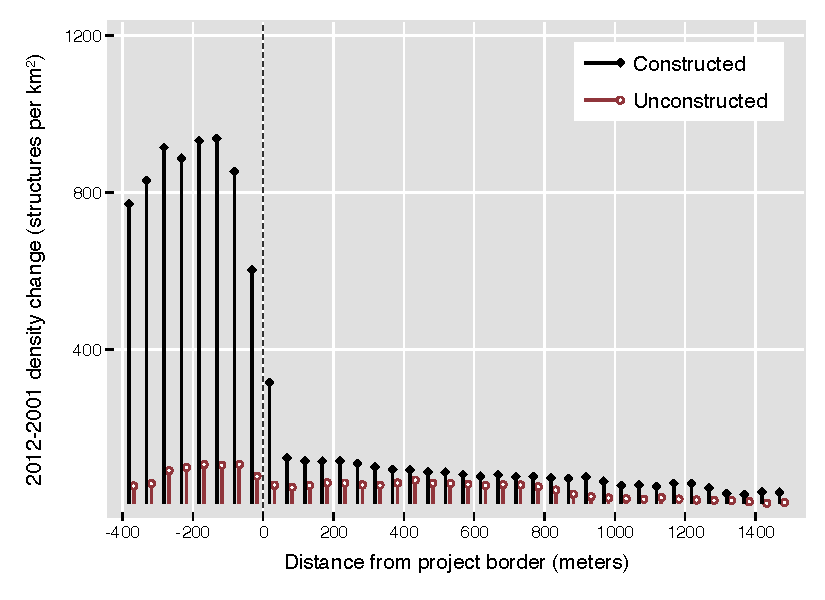
\includegraphics[width=\textwidth,trim={0.3cm .3cm 0.1cm 0cm}, clip=true]{figures/bblu_for_rawchanges_4_3_spk.pdf}

        \end{subfigure}
        \hfill
        \begin{subfigure}[b]{0.48\textwidth} 
                    \caption[]%
            {{\footnotesize \textbf{Other} changes informal  raw data}}      
            \label{fig:preinf} 
            \centering 
            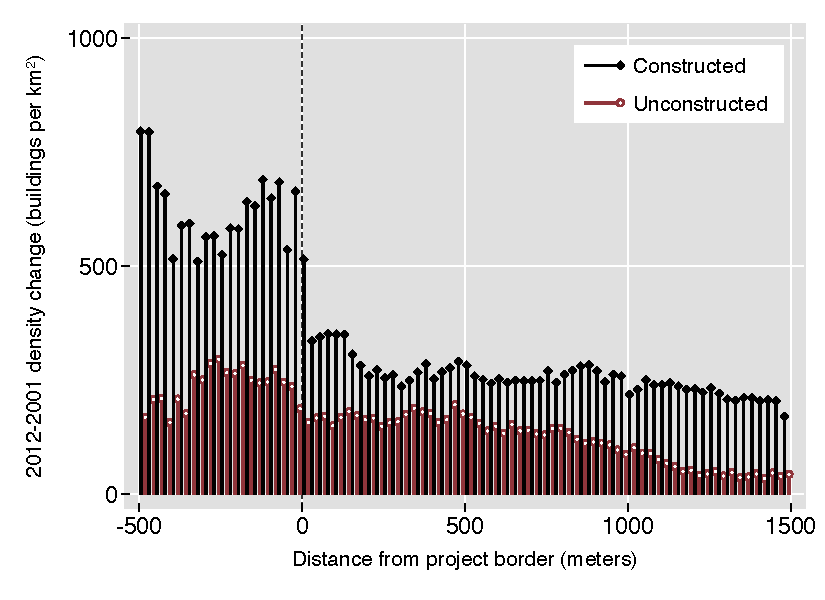
\includegraphics[width=\textwidth,trim={0.3cm .3cm 0.1cm 0cm}, clip=true]{figures/bblu_inf_rawchanges_4_3_spk.pdf}

        \end{subfigure}
\end{figure*}




\begin{table}[h!]
\small
\centering
\caption{Triple Difference Estimates of Housing Density }\label{table:bbluDDDfull}
\vspace{-2mm}
\begin{tabular}{lCCCCC}
\toprule
& \small (1) & \small (2) & \small (3) & \small (4)& \small (5) \\
 & \small Total Housing & \small Formal Housing & \small Total Informal Housing & \small Informal Backyard Housing & \small Informal Non-Bkyd. Housing \\ \midrule 
inside $\times$ constr $\times$ post&       618.4\textsuperscript{a}&       649.7\textsuperscript{a}&       -31.3                   &      -572.9\textsuperscript{a}&       541.6\textsuperscript{a}\\
                    &     (209.7)                   &     (108.4)                   &     (153.2)                   &     (144.1)                   &     (136.8)                   \\[0.01em]
0-500m away $\times$ constr $\times$ post&      -216.7\textsuperscript{b}&       -34.3                   &      -182.4\textsuperscript{b}&       -73.1                   &      -109.4                   \\
                    &     (110.4)                   &      (61.9)                   &      (92.7)                   &      (80.7)                   &      (80.7)                   \\[0.05em]
inside $\times$ post&       373.7\textsuperscript{b}&        80.8                   &       292.9\textsuperscript{b}&       277.1\textsuperscript{b}&        15.8                   \\
                    &     (146.0)                   &      (62.0)                   &     (122.0)                   &     (116.1)                   &      (65.6)                   \\[0.01em]
0-500m away $\times$ post&       473.2\textsuperscript{a}&       175.5\textsuperscript{a}&       297.7\textsuperscript{a}&        38.5                   &       259.1\textsuperscript{a}\\
                    &      (92.9)                   &      (57.1)                   &      (77.5)                   &      (75.6)                   &      (65.3)                   \\[0.05em]
constr $\times$ post&        77.4\textsuperscript{c}&         6.2                   &        71.2\textsuperscript{b}&       -17.2                   &        88.4\textsuperscript{a}\\
                    &      (41.6)                   &      (13.4)                   &      (36.0)                   &      (12.6)                   &      (33.4)                   \\[0.5em]
inside $\times$ constr&        45.6                   &         5.7                   &        39.9                   &       170.6\textsuperscript{b}&      -130.7\textsuperscript{b}\\
                    &     (103.9)                   &      (48.9)                   &      (87.5)                   &      (78.1)                   &      (57.3)                   \\[0.01em]
0-500m away $\times$ constr&       -17.7                   &       -29.7                   &        11.9                   &       -19.3                   &        31.3                   \\
                    &      (61.4)                   &      (43.3)                   &      (57.3)                   &      (55.0)                   &      (37.7)                   \\[0.05em]
post                &       171.2\textsuperscript{a}&        46.2\textsuperscript{a}&       125.0\textsuperscript{a}&        33.8\textsuperscript{a}&        91.2\textsuperscript{a}\\
                    &      (25.8)                   &       (9.6)                   &      (20.9)                   &       (8.6)                   &      (18.7)                   \\
inside              &      -167.8\textsuperscript{a}&      -163.8\textsuperscript{a}&        -3.9                   &        66.1                   &       -70.1\textsuperscript{b}\\
                    &      (61.4)                   &      (34.4)                   &      (47.0)                   &      (42.5)                   &      (29.0)                   \\[0.01em]
0-500m away         &      -116.2\textsuperscript{b}&       -57.4                   &       -58.8                   &        68.1                   &      -126.9\textsuperscript{a}\\
                    &      (52.0)                   &      (40.5)                   &      (50.5)                   &      (51.1)                   &      (30.4)                   \\[0.01em]
constr              &         3.7                   &        25.8                   &       -22.0                   &        -2.1                   &       -19.9                   \\
                    &      (33.7)                   &      (17.3)                   &      (24.0)                   &      (14.2)                   &      (17.7)                   \\[0.1em]
Mean Pre            &      579.36                   &      288.49                   &      290.87                   &      184.19                   &      106.68                   \\
Mean Post           &      922.93                   &      424.41                   &      498.52                   &      182.46                   &      316.06                   \\
R$^2$               &       0.322                   &       0.292                   &       0.276                   &       0.272                   &       0.200                   \\
N                   &   6,143,756                   &   6,143,756                   &   6,143,756                   &   6,143,756                   &   6,143,756                   \\

\bottomrule
\multicolumn{6}{l}{\footnotesize Standard errors clustered at the project level in parenthesis. \textsuperscript{c} p$<$0.10,\textsuperscript{b} p$<$0.05,\textsuperscript{a} p$<$0.01 }\\[-.3em]
\multicolumn{6}{l}{\footnotesize Project areas are 25$\times$25m grid cells within 1,500m of project footprints.}\\[-.3em]
\multicolumn{6}{l}{\footnotesize Housing densities are measure in terms of houses per $\text{km}^{2}$.}\\[-.3em]
\multicolumn{6}{l}{\footnotesize ``inside'' means within project footprint.  ``constr'' means constructed.} 
\end{tabular}
\end{table}






\end{document}


